% !TeX root = ../../Skript.tex
\cohead{\Large\textbf{Optimierungsaufgaben}}
\fakesubsection{Optimierungsaufgaben}
Bei Optimierungsaufgaben muss für eine Größe wie die Fläche eines Rechtecks oder Dreiecks die Länge einer Verbindungslinie das Optimum, also das Maximum/Minimum gefunden werden. Dazu müssen die folgenden Schritte durchgeführt werden (Je nach Aufgabenstellung sind nicht immer alle Schritte notwendig), die wir an Hand folgenden Beispiels näher betrachten werden:

\smallskip

\begin{minipage}{\textwidth}
	\adjustbox{valign=t, padding = 0ex 0ex 2ex 0ex}{\begin{minipage}{.5\textwidth-2ex}
		Gegeben ist die Funktion \(f(x)=-x^2+5x\). Sei \(P(u\vert v)\) ein Punkt auf dem Graphen von \(f\) mit \(0\leq u\leq 5\). Der Ursprung, der Punkt \(P\) und der Punkt \(Q(u\vert 0)\) begrenzen ein Dreieck. Welchen Flächeninhalt \(A\) kann dieses Dreieck maximal annehmen?
		\begin{enumerate}
			\item \textbf{Skizze}

			\textcolor{loes}{Eine Skizze sollte immer angefertigt werden.}
			\item \textbf{Zielfunktion aufstellen}

			\textcolor{loes}{Die Zielfunktion gibt Wert der zu optimierenden Größe in Abhängigkeit einer Variablen (meistens \(u\)) an. Im Beispiel kann man die Form des Dreiecks ändern, indem man die Variable \(u\) ändert. Die zu optimierende Größe ist der Flächeninhalt \(A\) des Dreiecks. Wir suchen also eine Funktion \(A(u)\):}
		\end{enumerate}
	\end{minipage}}%
	\adjustbox{valign=t, padding = 2ex 0ex 0ex 0ex}{\begin{minipage}{.5\textwidth-2ex}
        \iftoggle{qrcode}{
		\settototalheight{\imgheight}{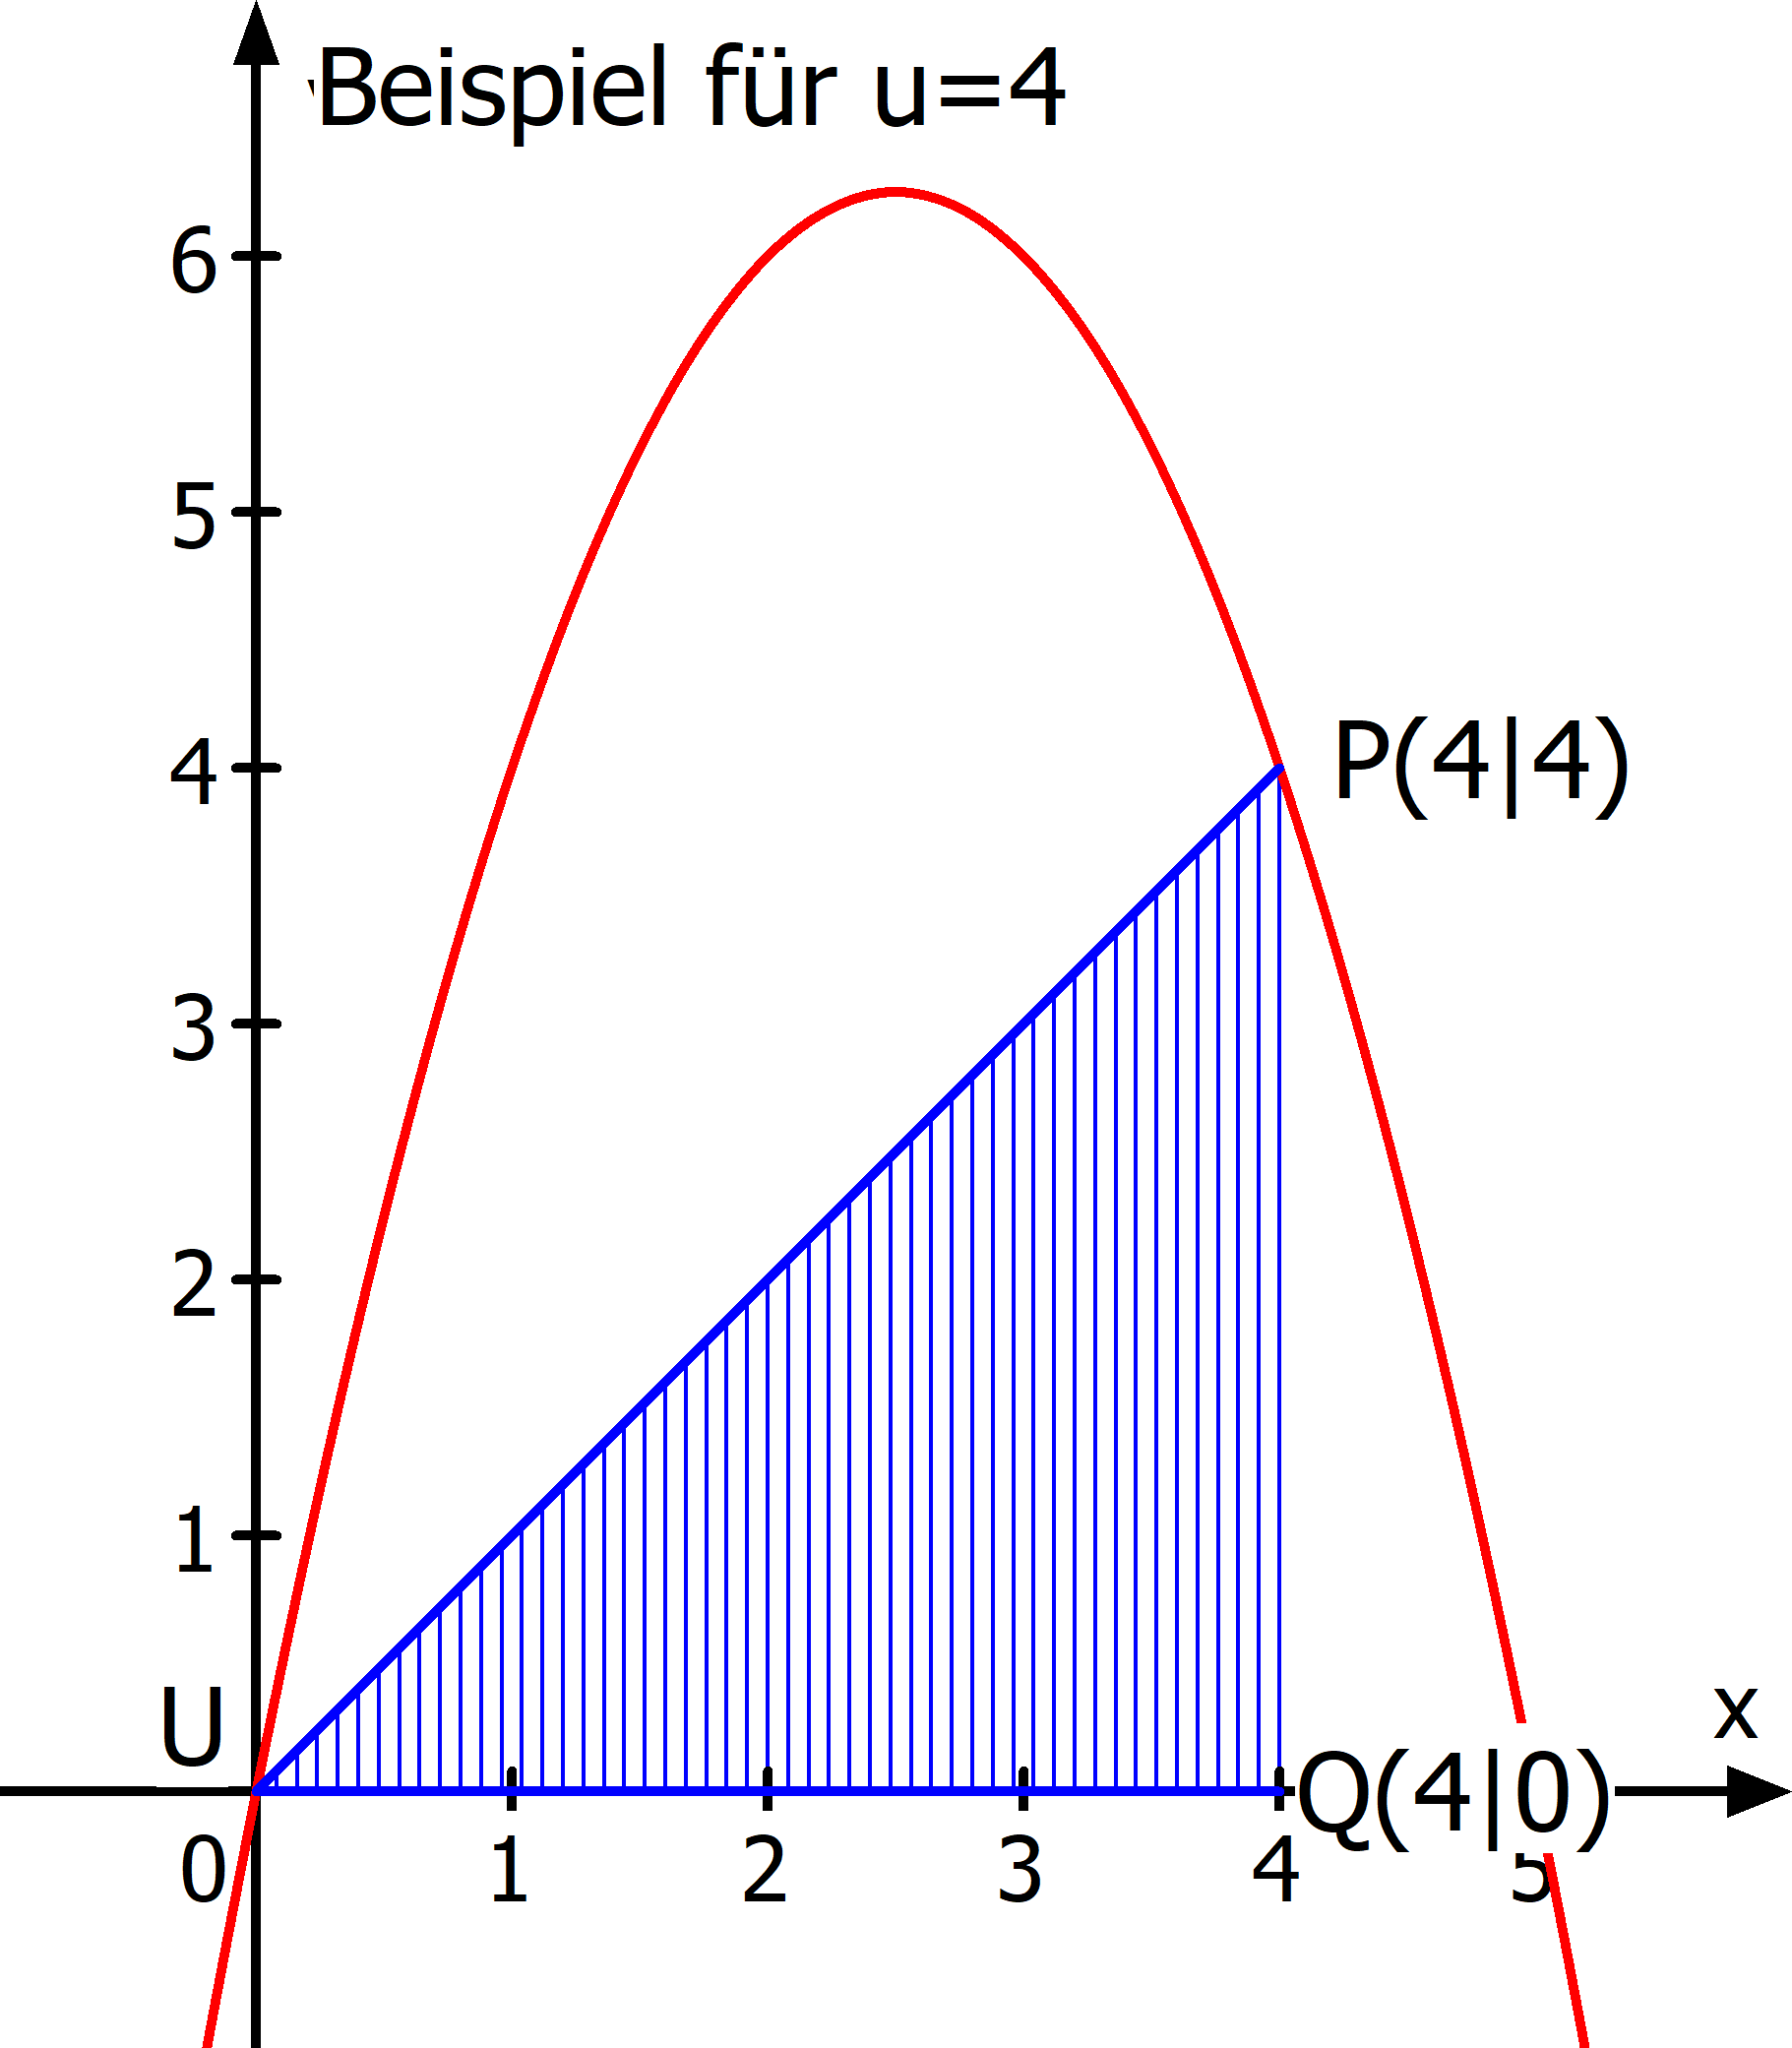
\includegraphics[width=\linewidth]{\optimierung/pics/Beispiel1.png}}%
        \setlength{\qrheight}{2.5cm}%
        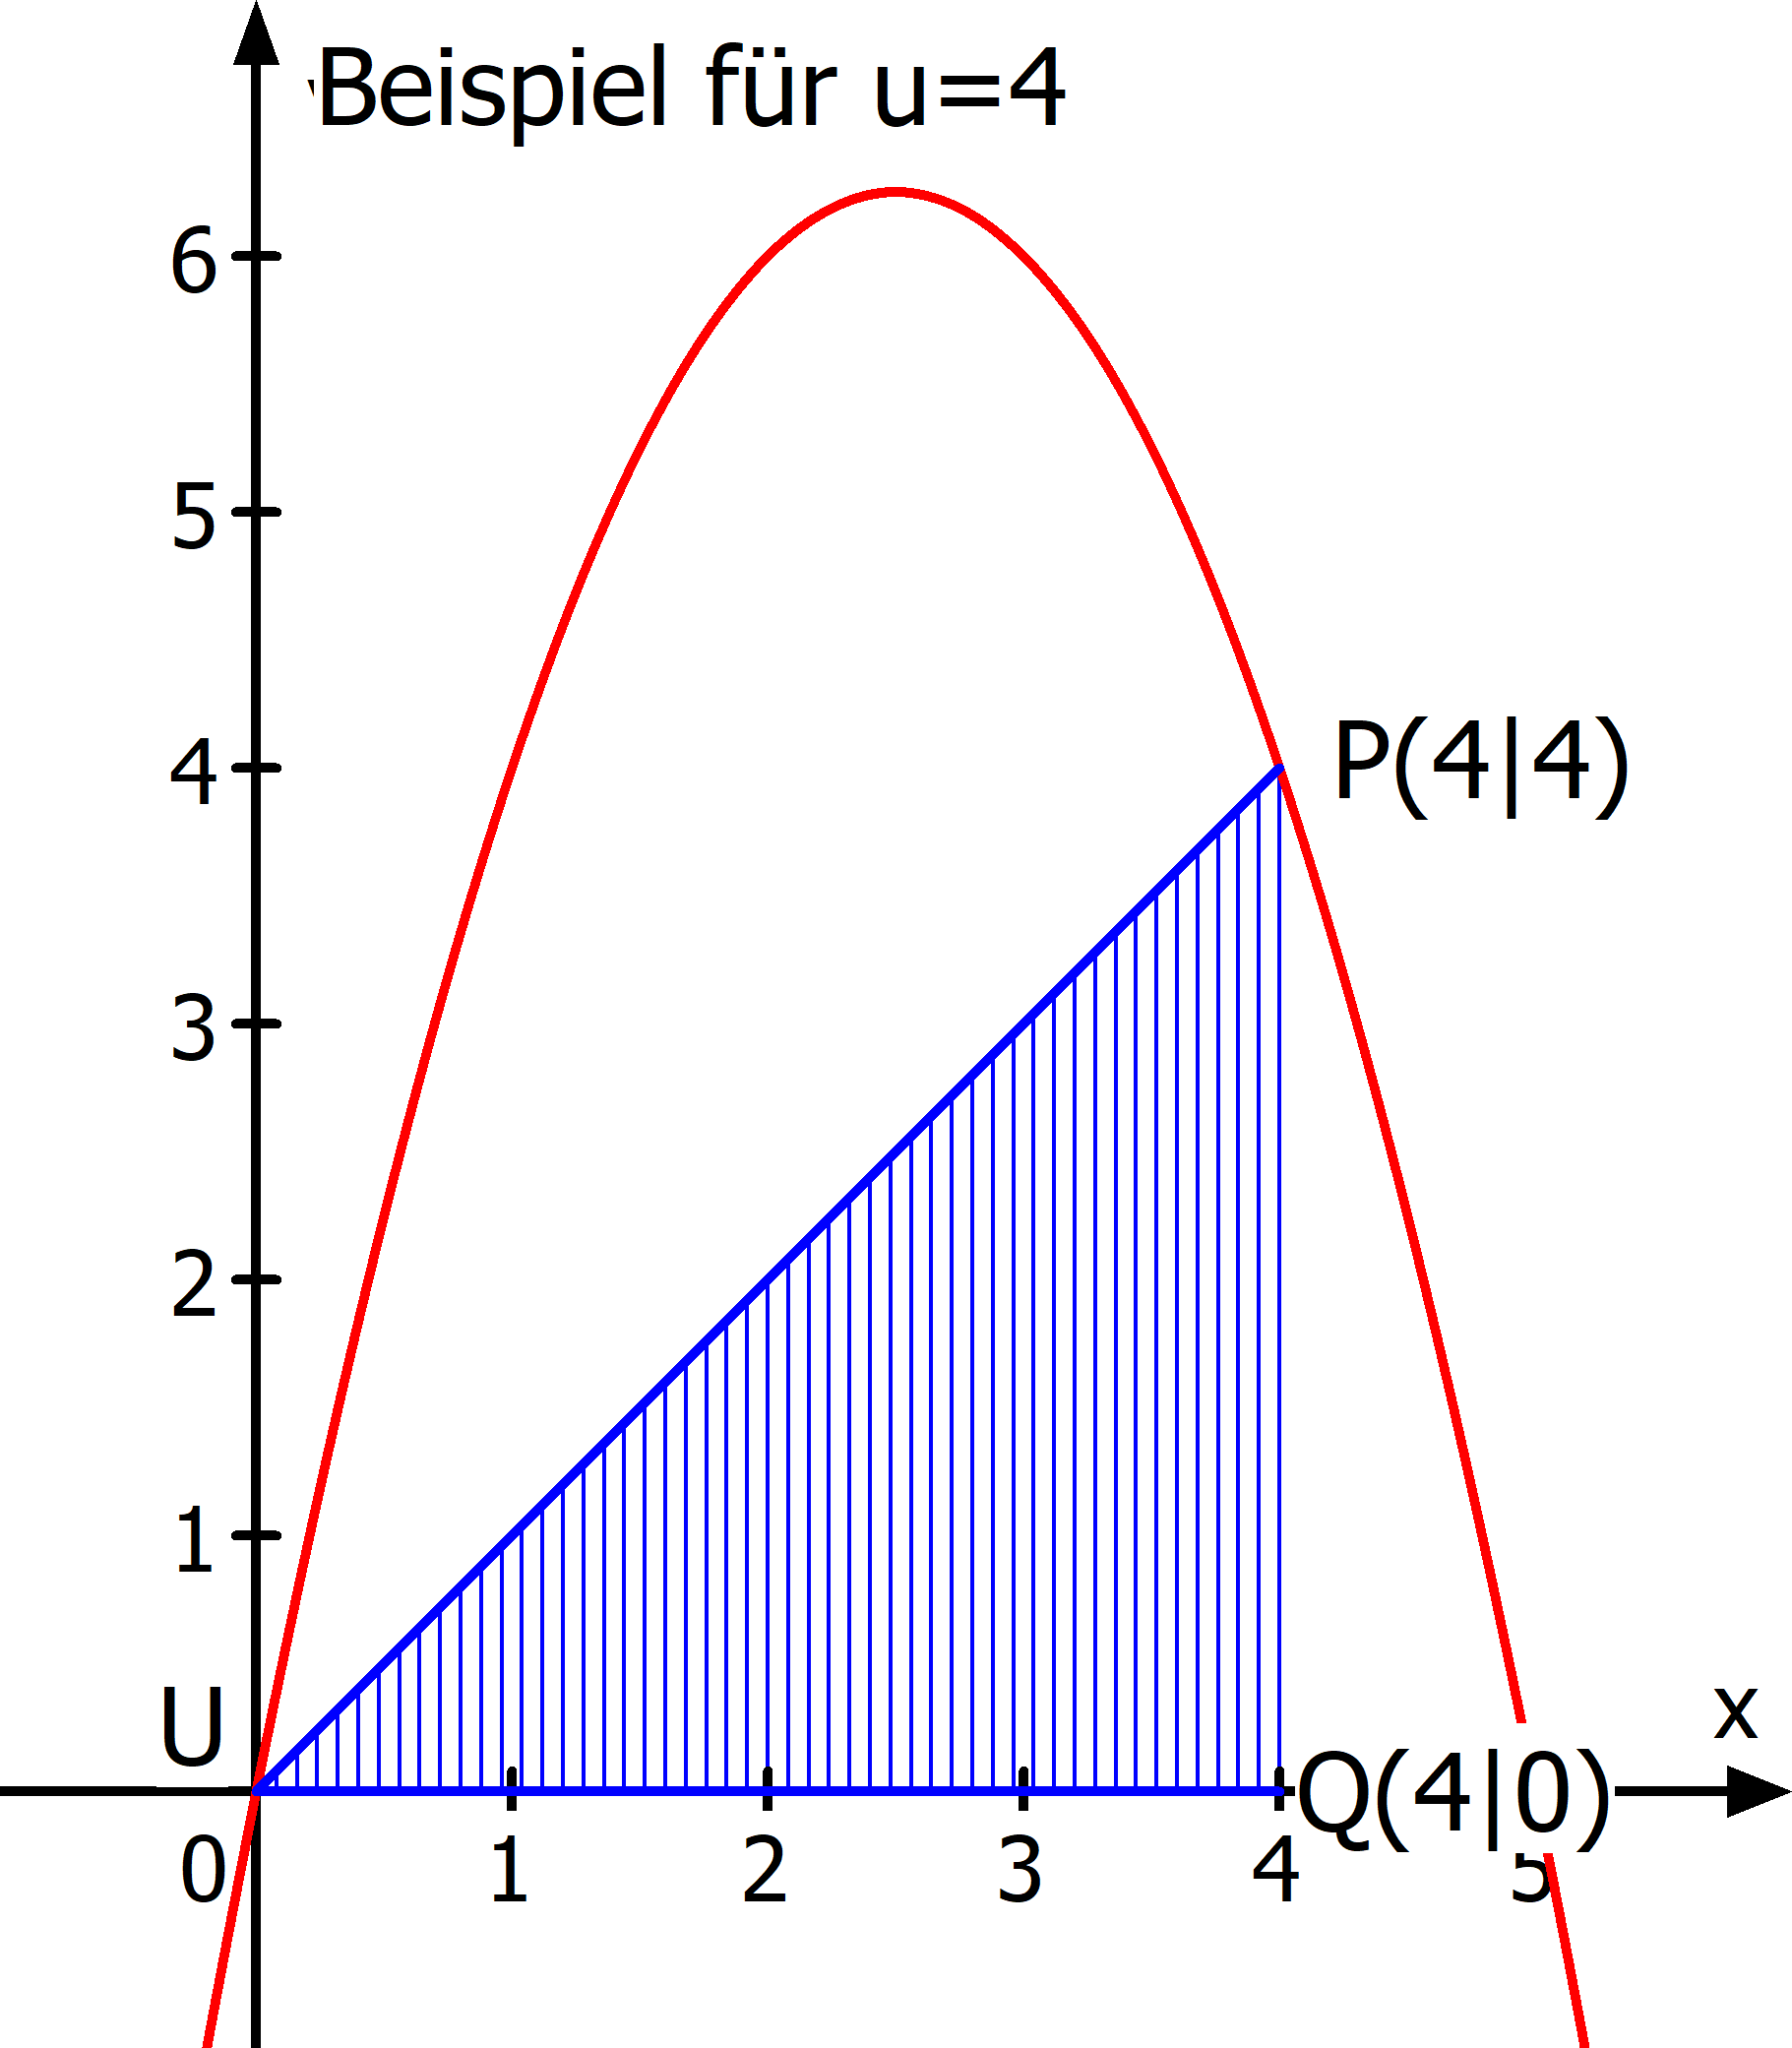
\includegraphics[width=\linewidth]{\optimierung/pics/Beispiel1.png}%
        \raisebox{\imgheight-\qrheight}{\makebox[0pt][r]{\href{https://www.geogebra.org/m/cxbqrqxz}{
\includegraphics[height=\qrheight]{\optimierung/pics/Beispiel1QR.png}}}}%
        }{
        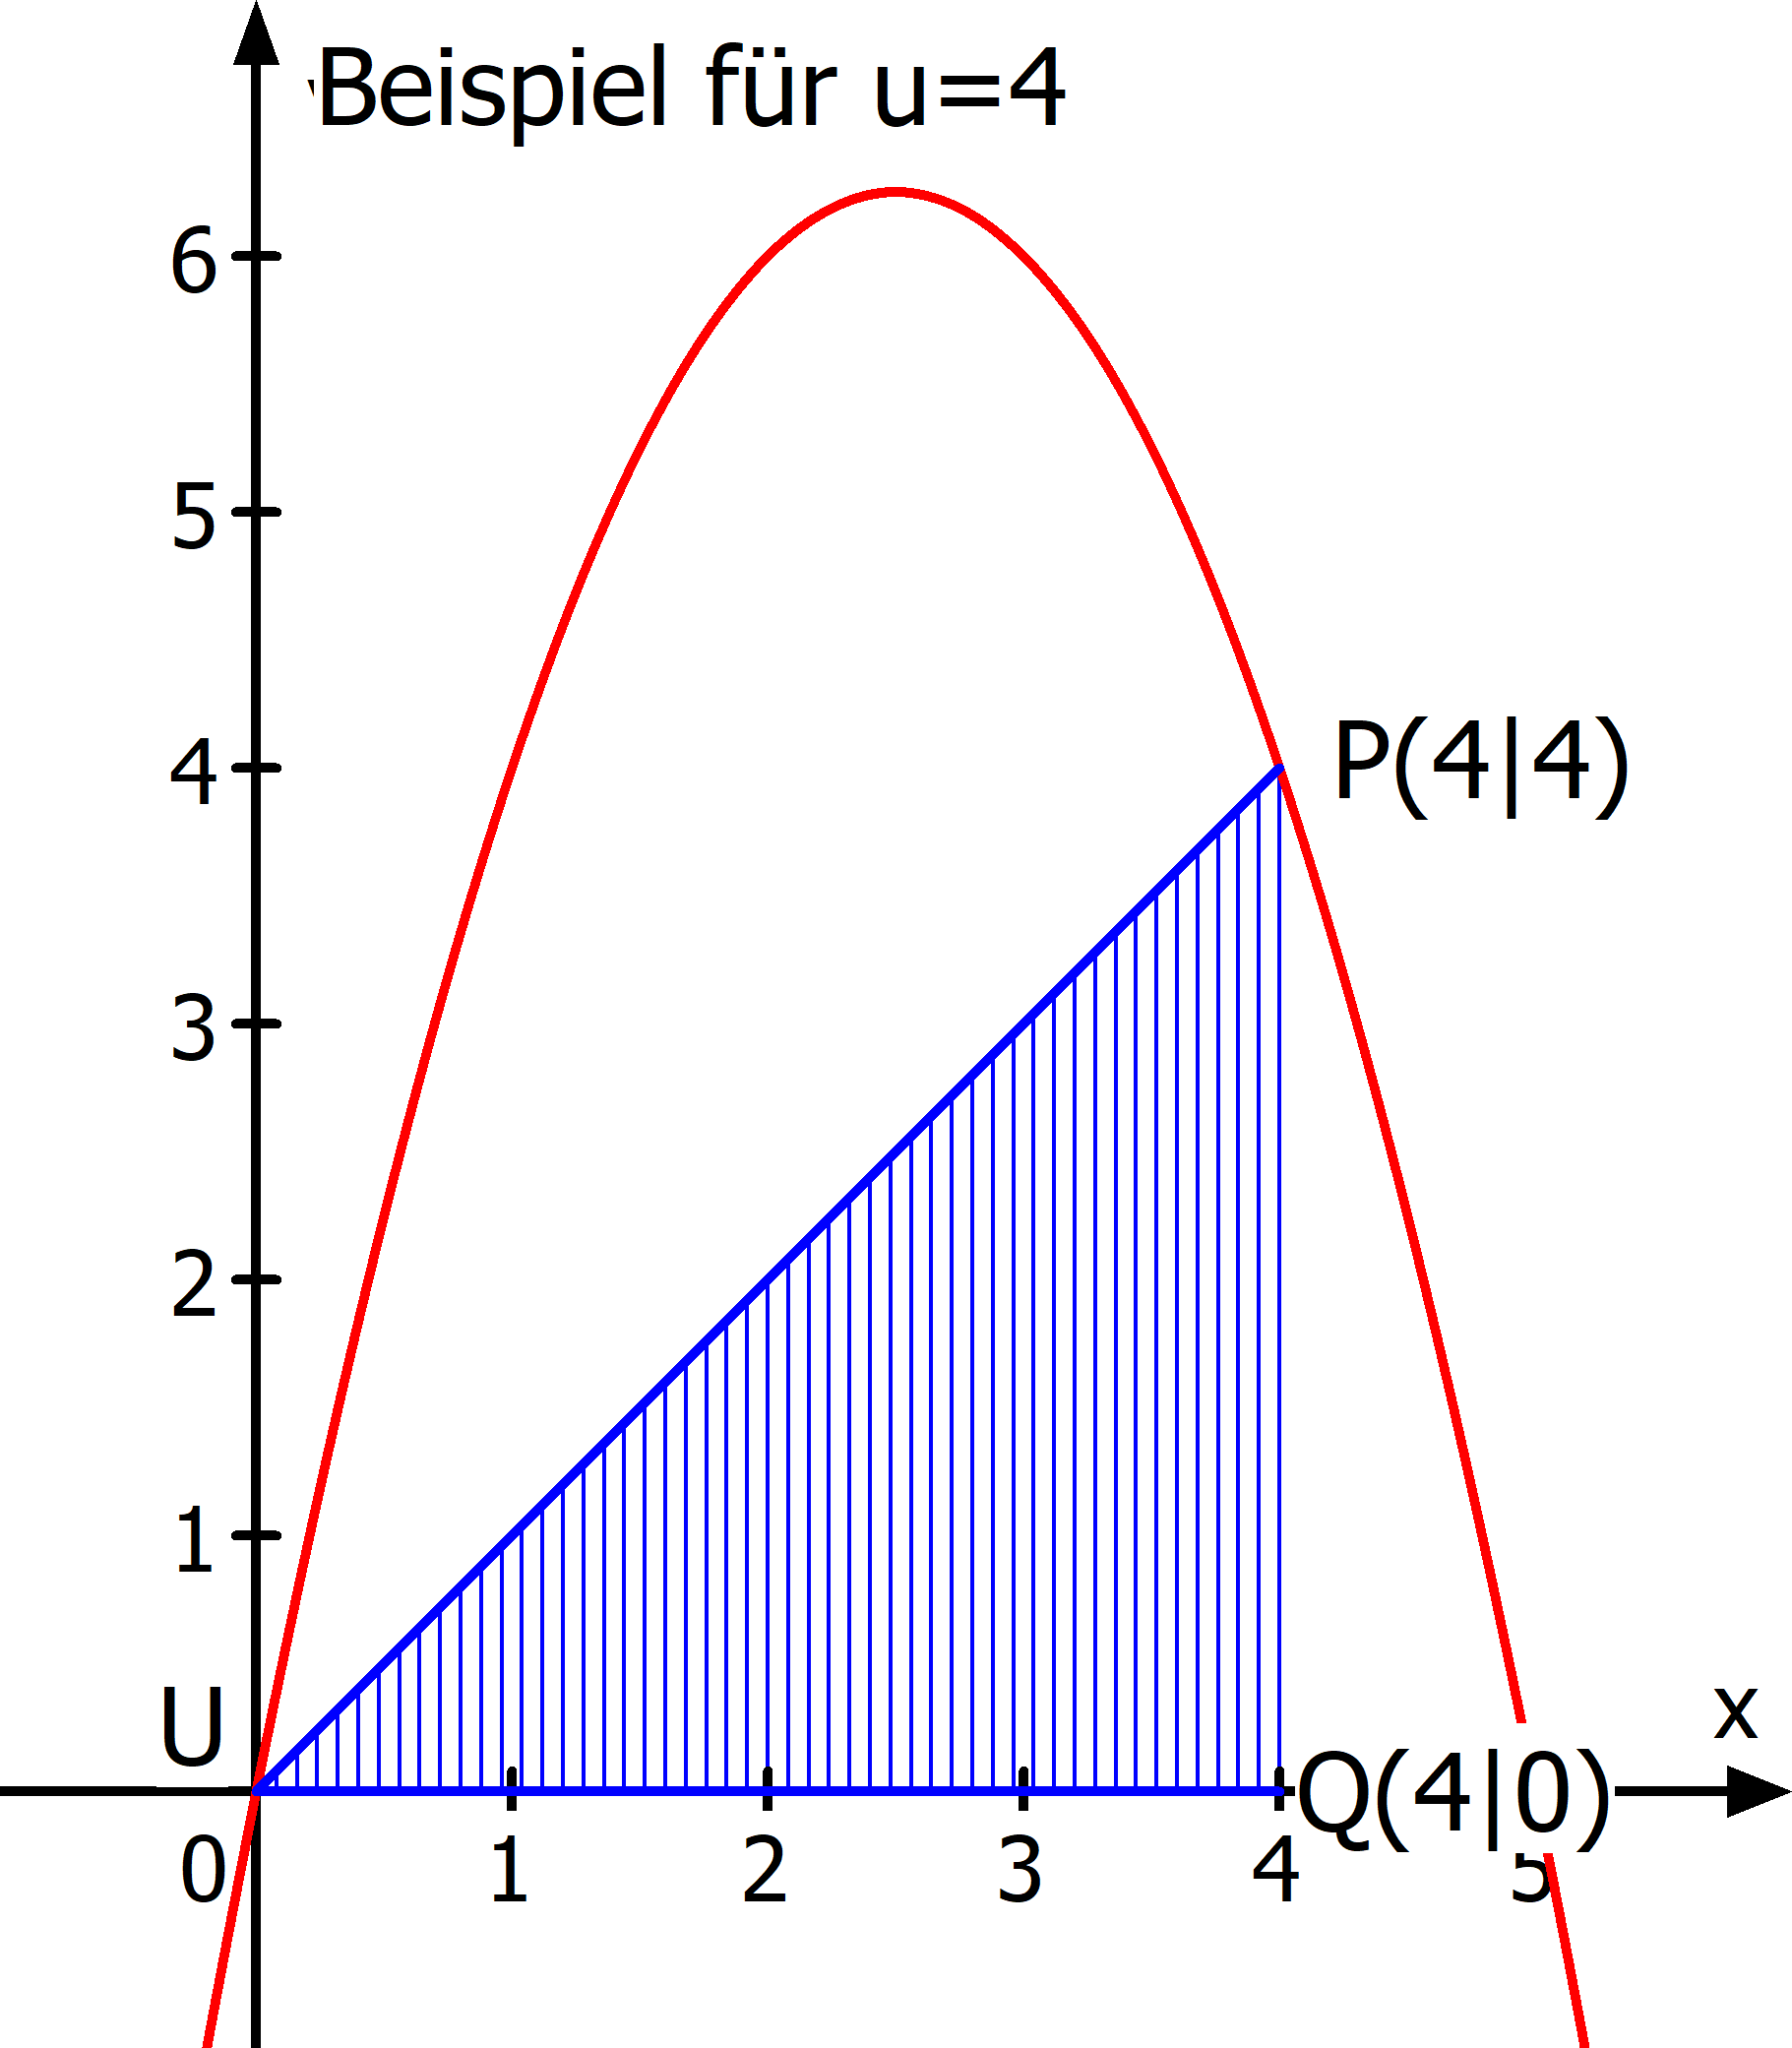
\includegraphics[width=\linewidth]{\optimierung/pics/Beispiel1.png}}%
	\end{minipage}}%
\end{minipage}
\textcolor{loes}{\[A(u)=\frac{1}{2}a\cdot h_a=\frac{1}{2}u\cdot f(u)=\frac{1}{2}u\left(-u^2+5u\right)=-\frac{1}{2}u^3+\frac{5}{2}u^2\]}
\begin{enumerate}
	\setcounter{enumi}{2}
	\item \textbf{Extremstellen der Zielfunktion bestimmen}

	\textcolor{loes}{Das Ziel ist das Maximum bzw. Minimum einer Größe zu bestimmen. Die Zielfunktion gibt uns alle möglichen Werte dieser Größe an. Das Maximum bzw. Minimum bestimmen wir wie üblich mit Hilfe der ersten und zweiten Ableitung:}
    \begin{align*}
	   \textcolor{loes}{A'(u)}&\textcolor{loes}{\;=-\frac{3}{2}u^2+5u}\\
	   \textcolor{loes}{A''(u)}&\textcolor{loes}{\;=-3u+5}\\
	   \textcolor{loes}{A'(u)}&\textcolor{loes}{\;=0\Rightarrow u_1=0\text{ und }u_2=\frac{10}{3}}\\
	   \textcolor{loes}{A''(0)}&\textcolor{loes}{\;=5>0\Rightarrow\text{ Tiefpunkt und }A''\left(\frac{10}{3}\right)=-5<0\Rightarrow\text{ Hochpunkt}}
    \end{align*}

	\item \textbf{Antwort erstellen}\\
	\textcolor{loes}{Vor dem Erstellen der Antwort sollte die Aufgabenstellung nochmals genau durchgelesen werden. In diesem Fall ist der maximale Flächeninhalt gesucht, der bei \(u_2=\frac{10}{3}\) liegt.}\\
	\textcolor{loes}{Der maximale Flächeninhalt beträgt}\\
	\textcolor{loes}{\[A_{max}=A\left(\tfrac{10}{3}\right)=-\frac{1}{2}\left(\frac{10}{3}\right)^3+\frac{5}{2}\left(\frac{10}{3}\right)^2=\frac{250}{27}\]}
\end{enumerate}

\begin{Exercise}[title={\raggedright\normalfont\\Gegeben ist die Funktion \(f(x)=-x^2+4x\). Sei \(P(u\vert v)\) ein Punkt auf dem Graphen von \(f\) mit \(0\leq u\leq4\). Der Ursprung, der Punkt \(P\) und der Punkt \(Q(u\vert 0)\) begrenzen ein Dreieck. Welchen Flächeninhalt A kann dieses Dreieck maximal haben?}, label=optimierungA1]\end{Exercise}
\begin{Exercise}[title={\raggedright\normalfont\\Gegeben ist die Funktion \(f(x)=-x^2+12\). Berechne die Koordinaten der Eckpunkte desjenigen Rechtecks oberhalb der x-Achse, dessen Flächeninhalt maximal ist, wenn eine Seite des Rechtecks auf der \(x\)-Achse liegt und 2 Eckpunkte auf dem Schaubild von \(f\) liegen. Gib den maximalen Flächeninhalt an. }, label=optimierungA2]\end{Exercise}
\begin{Exercise}[title={\raggedright\normalfont\\Die Graphen zu den beiden Funktionen mit \(f(x)=x^2\) und \(g(x)=-x^2+6\) schließen eine Fläche ein. In diese Fläche wird ein Rechteck so gelegt, dass die Rechteckseiten parallel zu den Koordinatenachsen verlaufen. Berechne die Koordinaten der Eckpunkte desjenigen Rechtecks, dessen Flächeninhalt maximal ist, und gib den maximalen Flächeninhalt an. }, label=optimierungA3]\end{Exercise}
\begin{Exercise}[title={\raggedright\normalfont\\Gegeben ist die Funktion \(f\) mit \(f(x)=(x-3)^2\). Betrachtet werden sollen alle achsenparallelen Rechtecke mit dem Ursprung als einen Eckpunkt und einem Punkt des Graphen als gegenüber liegendem Eckpunkt für \(0\leq x\leq 3\). Berechne die Koordinaten der Eckpunkte desjenigen Rechtecks, dessen Flächeninhalt maximal ist, und gib den maximalen Flächeninhalt an.}, label=optimierungA4]\end{Exercise}
\begin{Exercise}[title={\raggedright\normalfont\\Der Graph zu der Funktion mit \(f(x)=-kx^2+12,\ k>0\) und die \(x\)-Achse schließen eine Fläche ein. In diese Fläche wird ein Rechteck so gelegt, dass die Rechteckseiten parallel zu den Koordinatenachsen verlaufen. Berechne die Koordinaten der Eckpunkte desjenigen Rechtecks, dessen Flächeninhalt maximal ist in Abhängigkeit von \(k\), und gib den maximalen Flächeninhalt an.}, label=optimierungA5]\end{Exercise}


%%%%%%%%%%%%%%%%%%%%%%%%%%%%%%%%%%%%%%%%%
\begin{Answer}[ref=optimierungA1]

    \bigskip

	\begin{minipage}{\textwidth}
		\adjustbox{valign=t}{\begin{minipage}{.5\textwidth}\raggedright
			\textbf{Zielfunktion}

			\(A(u)=\frac{1}{2}u\cdot f(u)=-\frac{1}{2}u^3+u^2\)

			\textbf{Extremstellen der Zielfunktion}

			\(A'(u)=-\frac{3}{2}u^2+4u\)

			\(A''(u)=-3u+4\)

			\(A'(u)=0\) liefert \(u_1=0\) und \(u_2=\frac{8}{3}\)

			Mit \(A''(0)=4>0\) liegt bei \(u_1\) ein Tiefpunkt und mit \(A''\left(\frac{8}{3}\right)=-4<0\) liegt bei \(u_2\) ein Hochpunkt.

			\textbf{Antwort erstellen}

			Der maximale Flächeninhalt beträgt \(A\left(\frac{8}{3}\right)=\frac{128}{27}\)
		\end{minipage}}%
		\adjustbox{valign=t, padding = 2ex 0ex 0ex 0ex}{\begin{minipage}{.5\textwidth-2ex}
                \iftoggle{qrcode}{
                    \settototalheight{\imgheight}{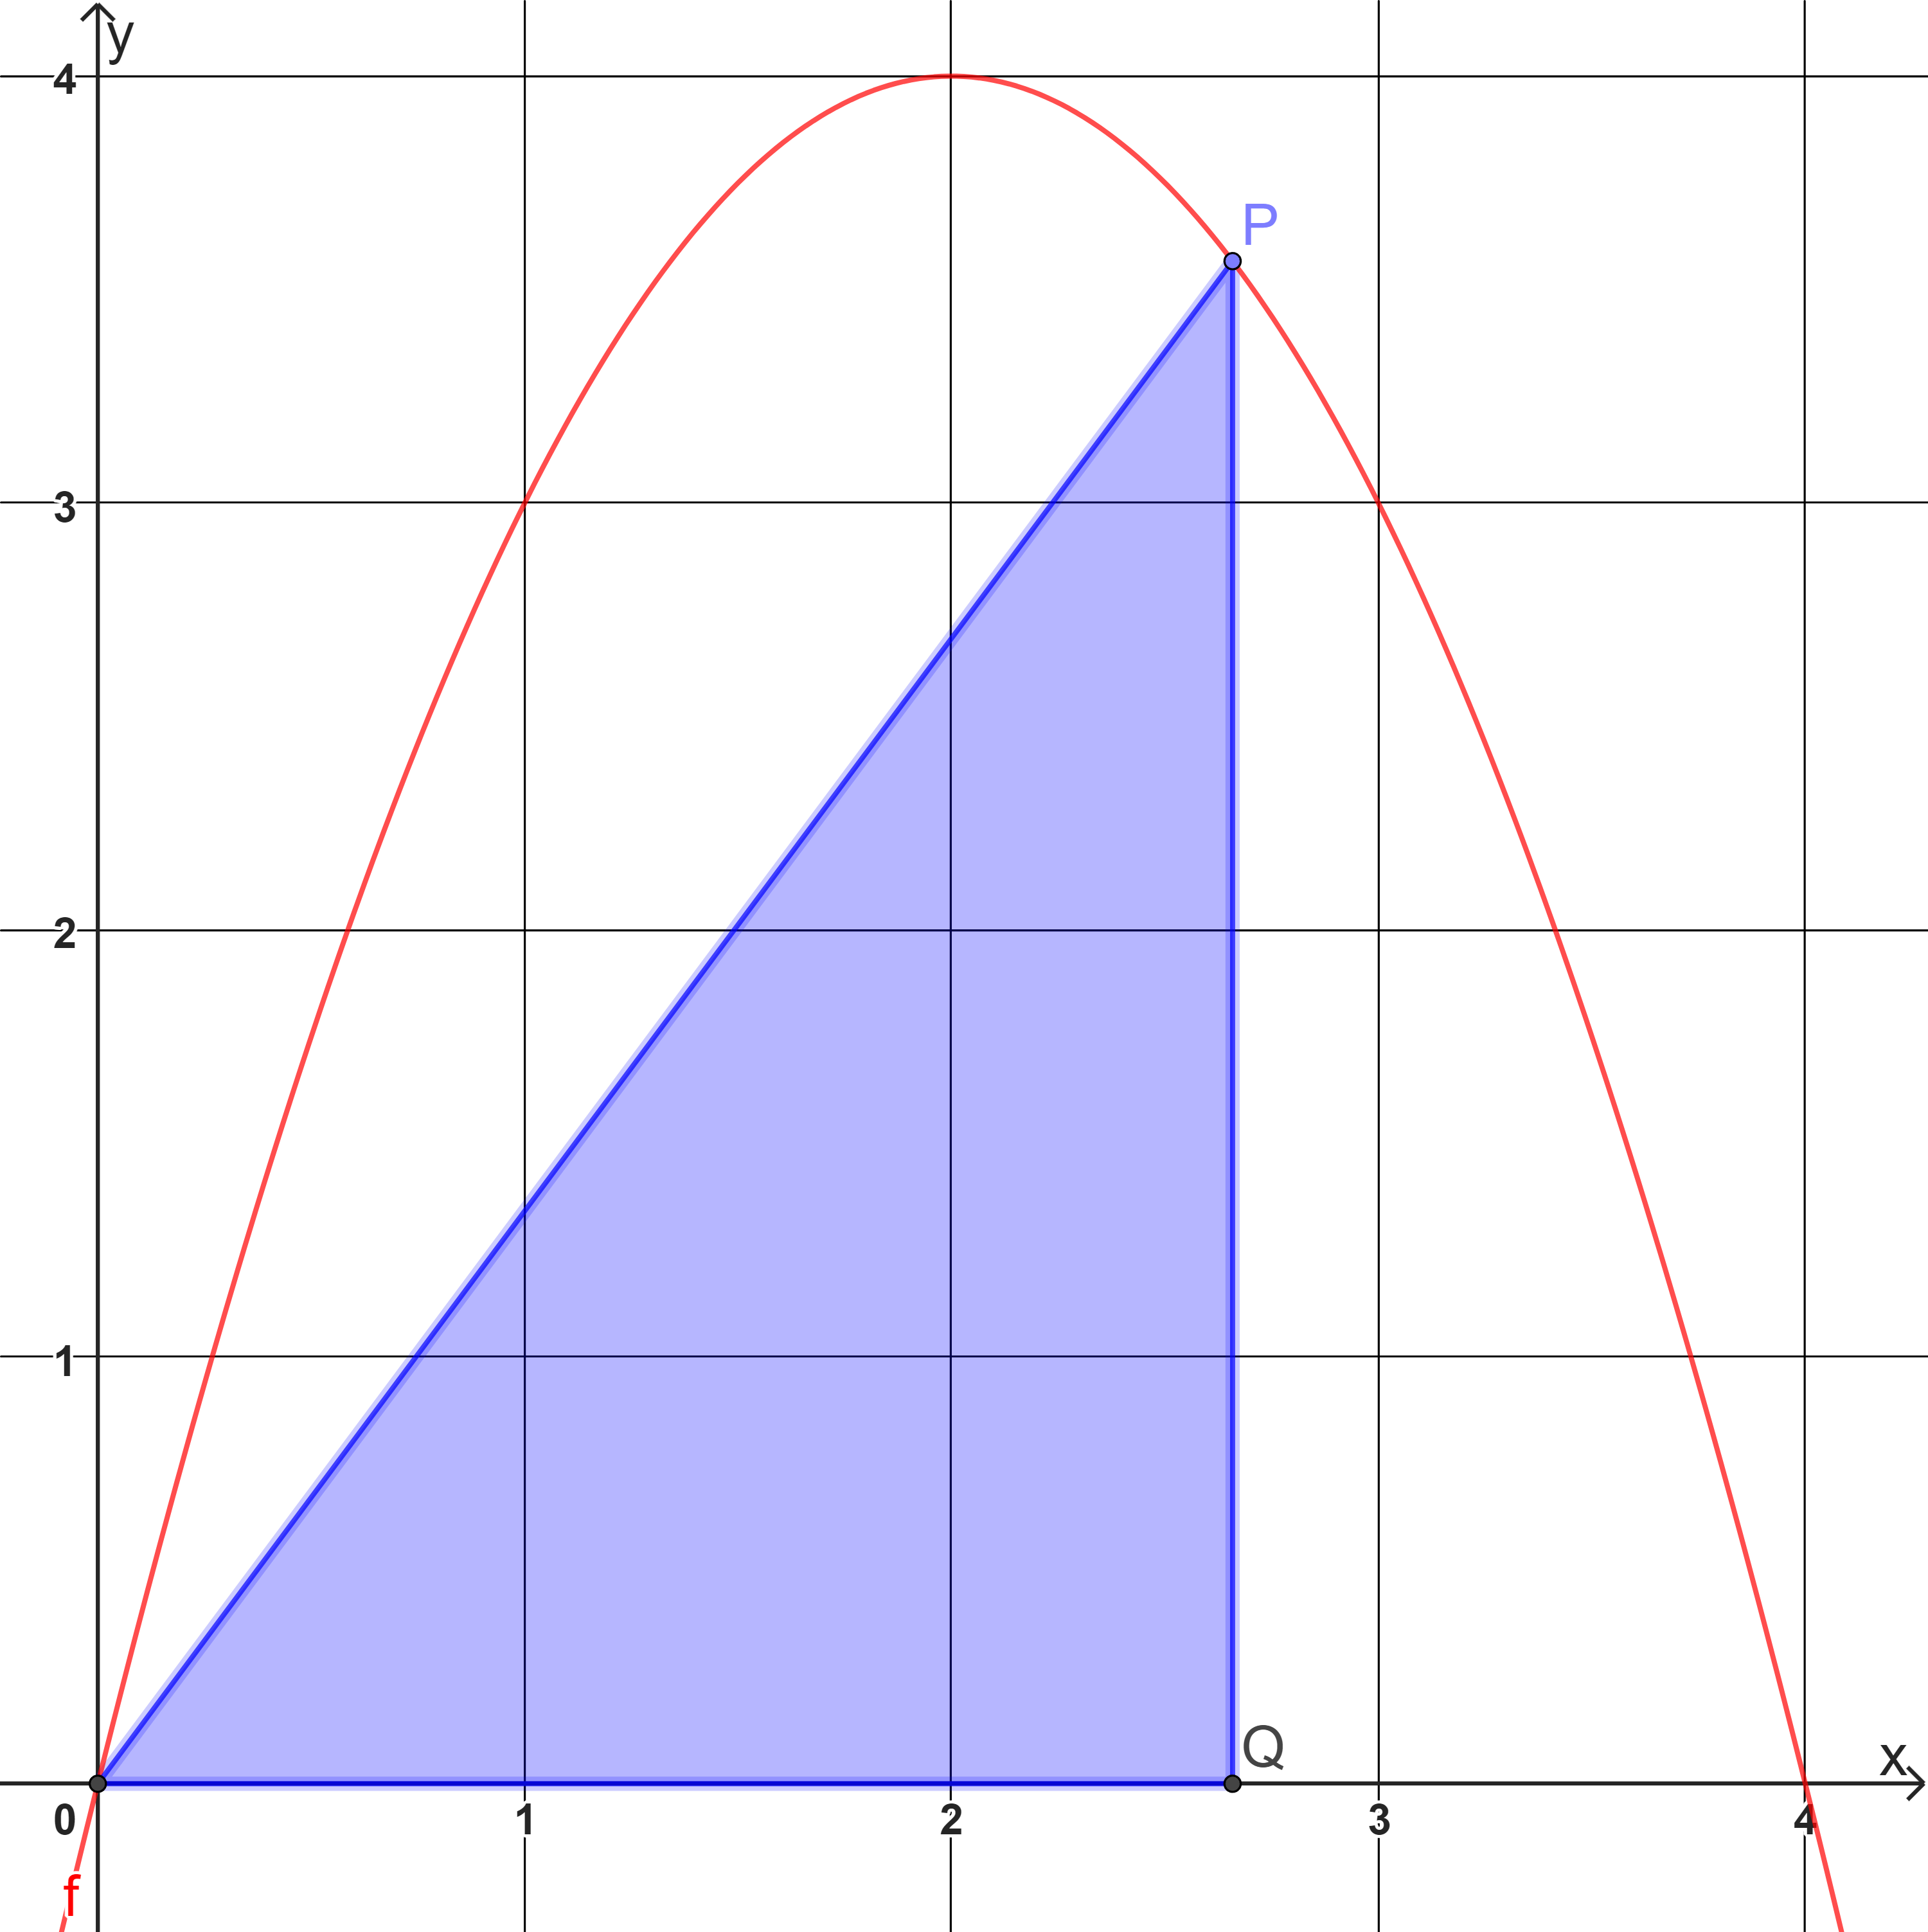
\includegraphics[width=\linewidth]{\optimierung/pics/Aufgabe_1.png}}%
                    \setlength{\qrheight}{2.5cm}%
                    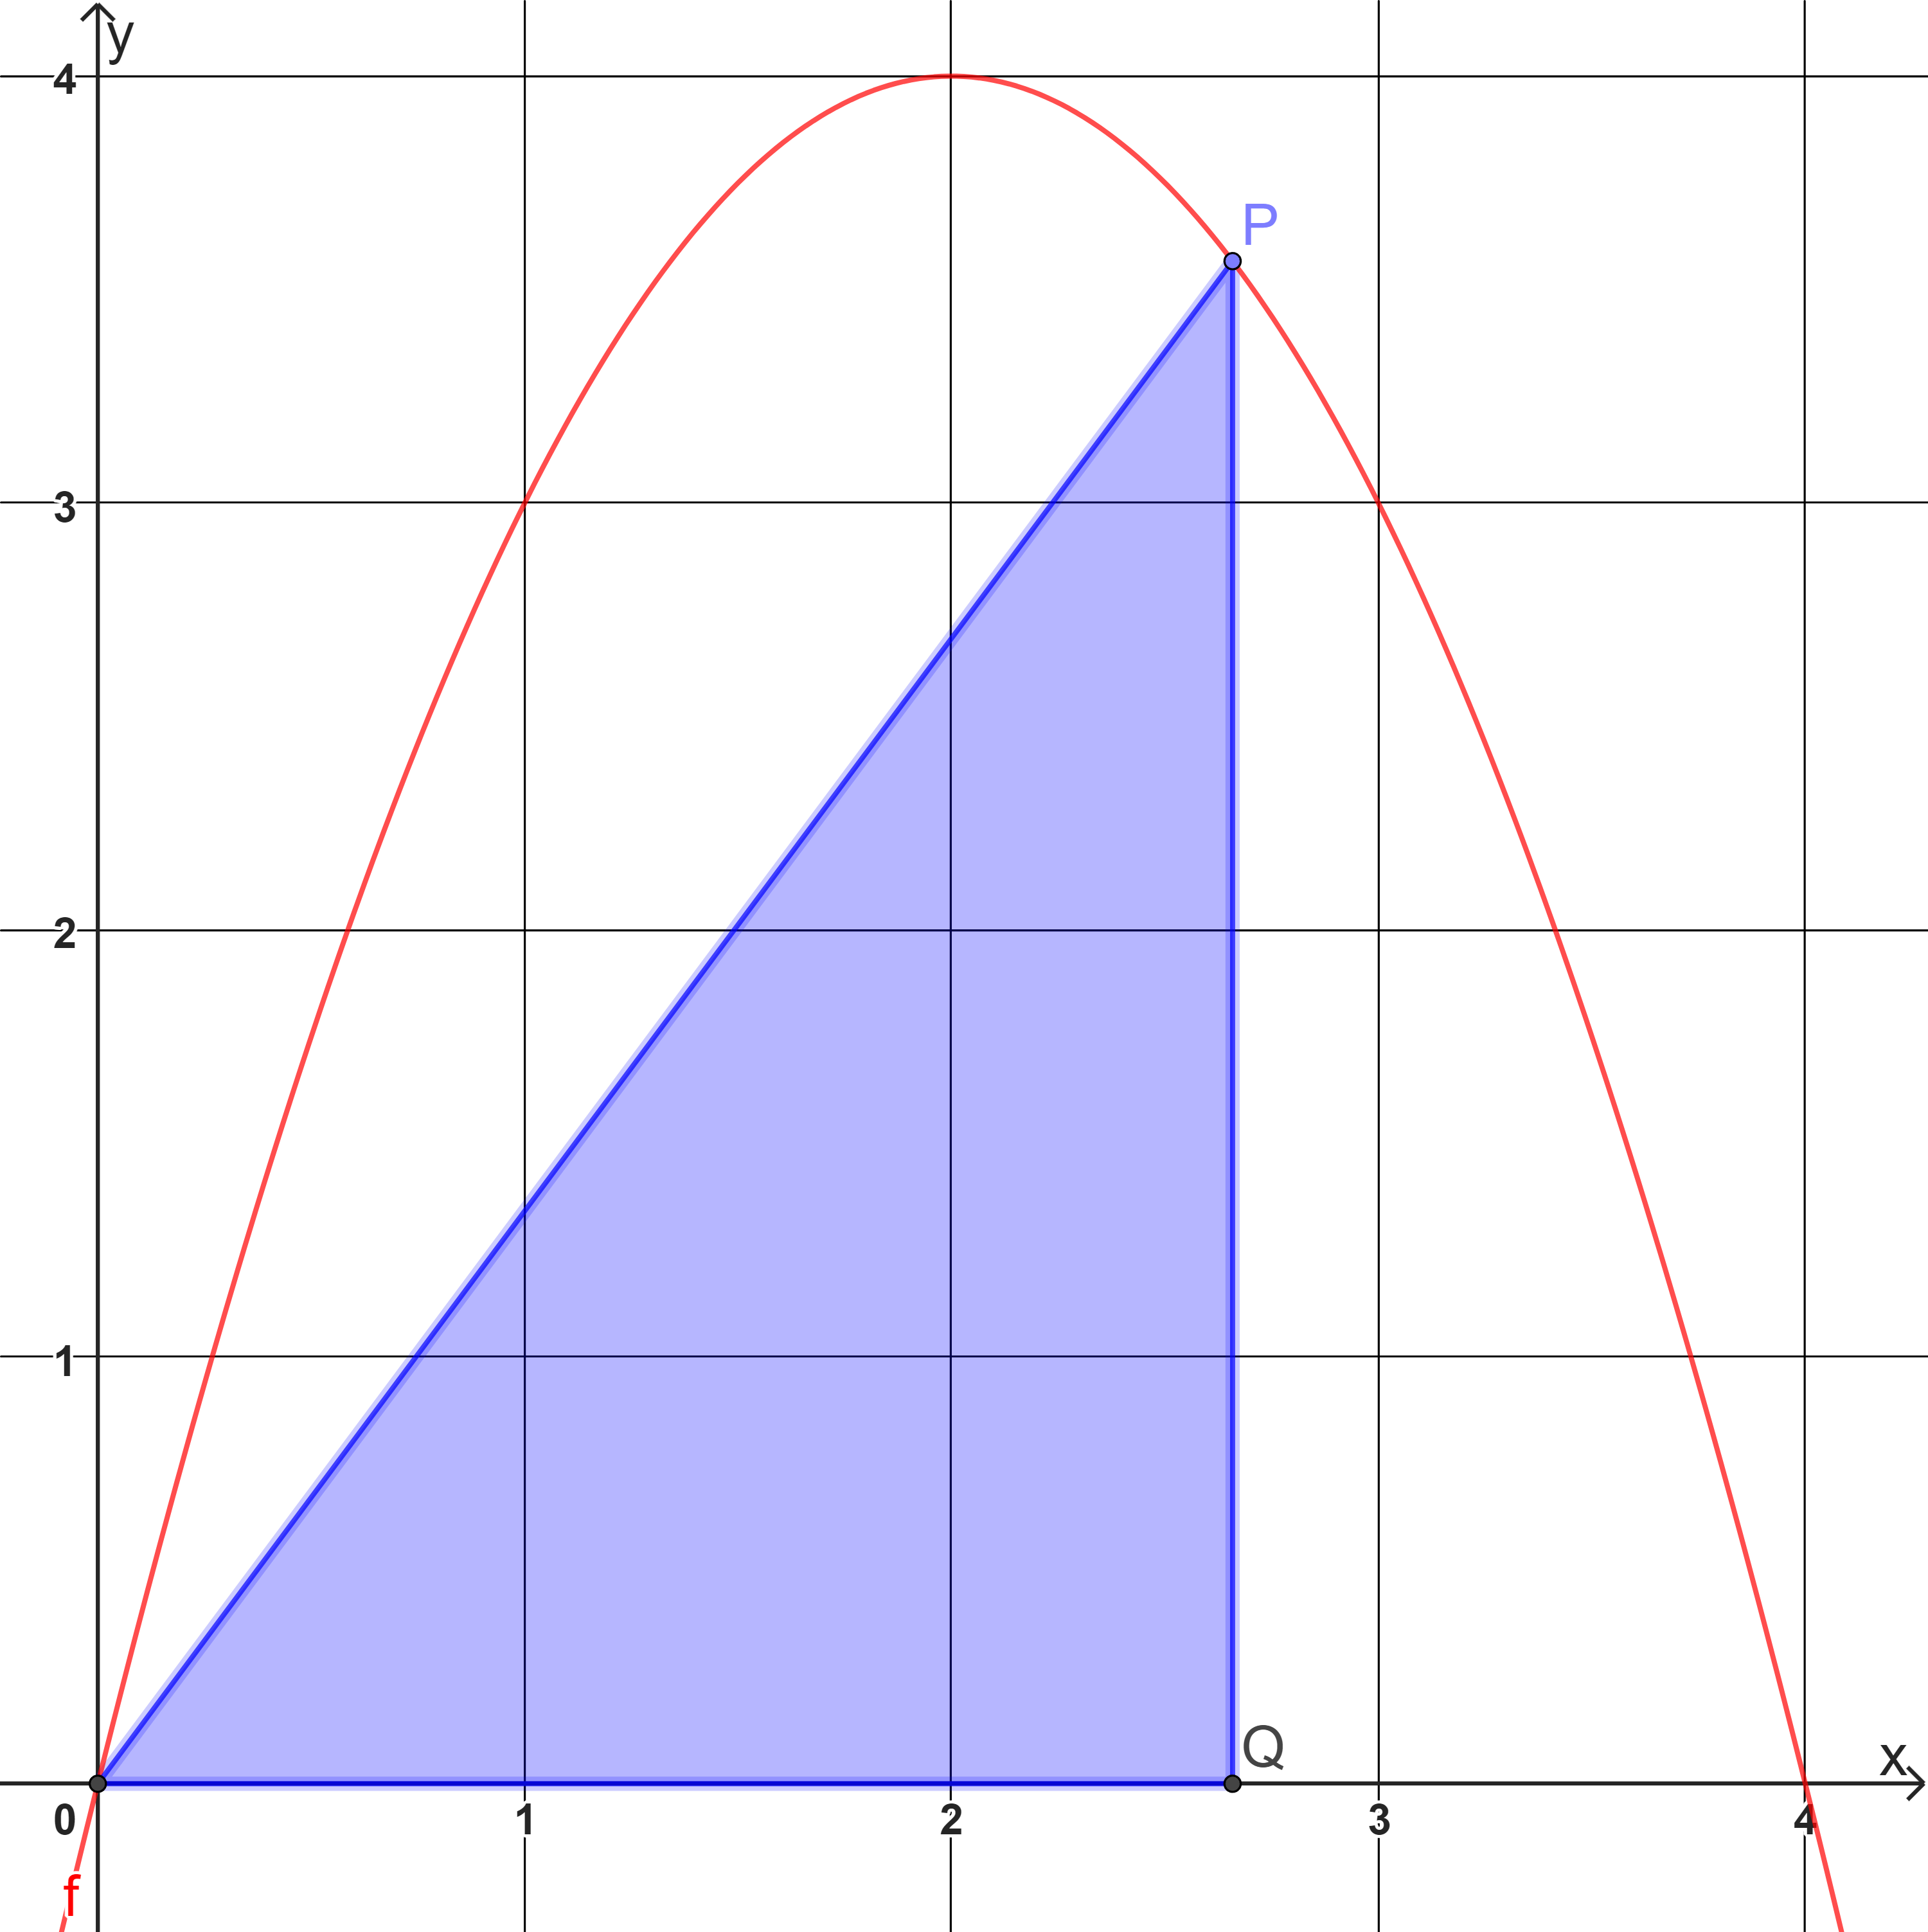
\includegraphics[width=\linewidth]{\optimierung/pics/Aufgabe_1.png}%
                    \raisebox{\imgheight-\qrheight}{\makebox[0pt][r]{\href{https://www.geogebra.org/m/bpm6d9z7}{
\includegraphics[height=\qrheight]{\optimierung/pics/Aufgabe_1QR.png}}}}%
                }{
			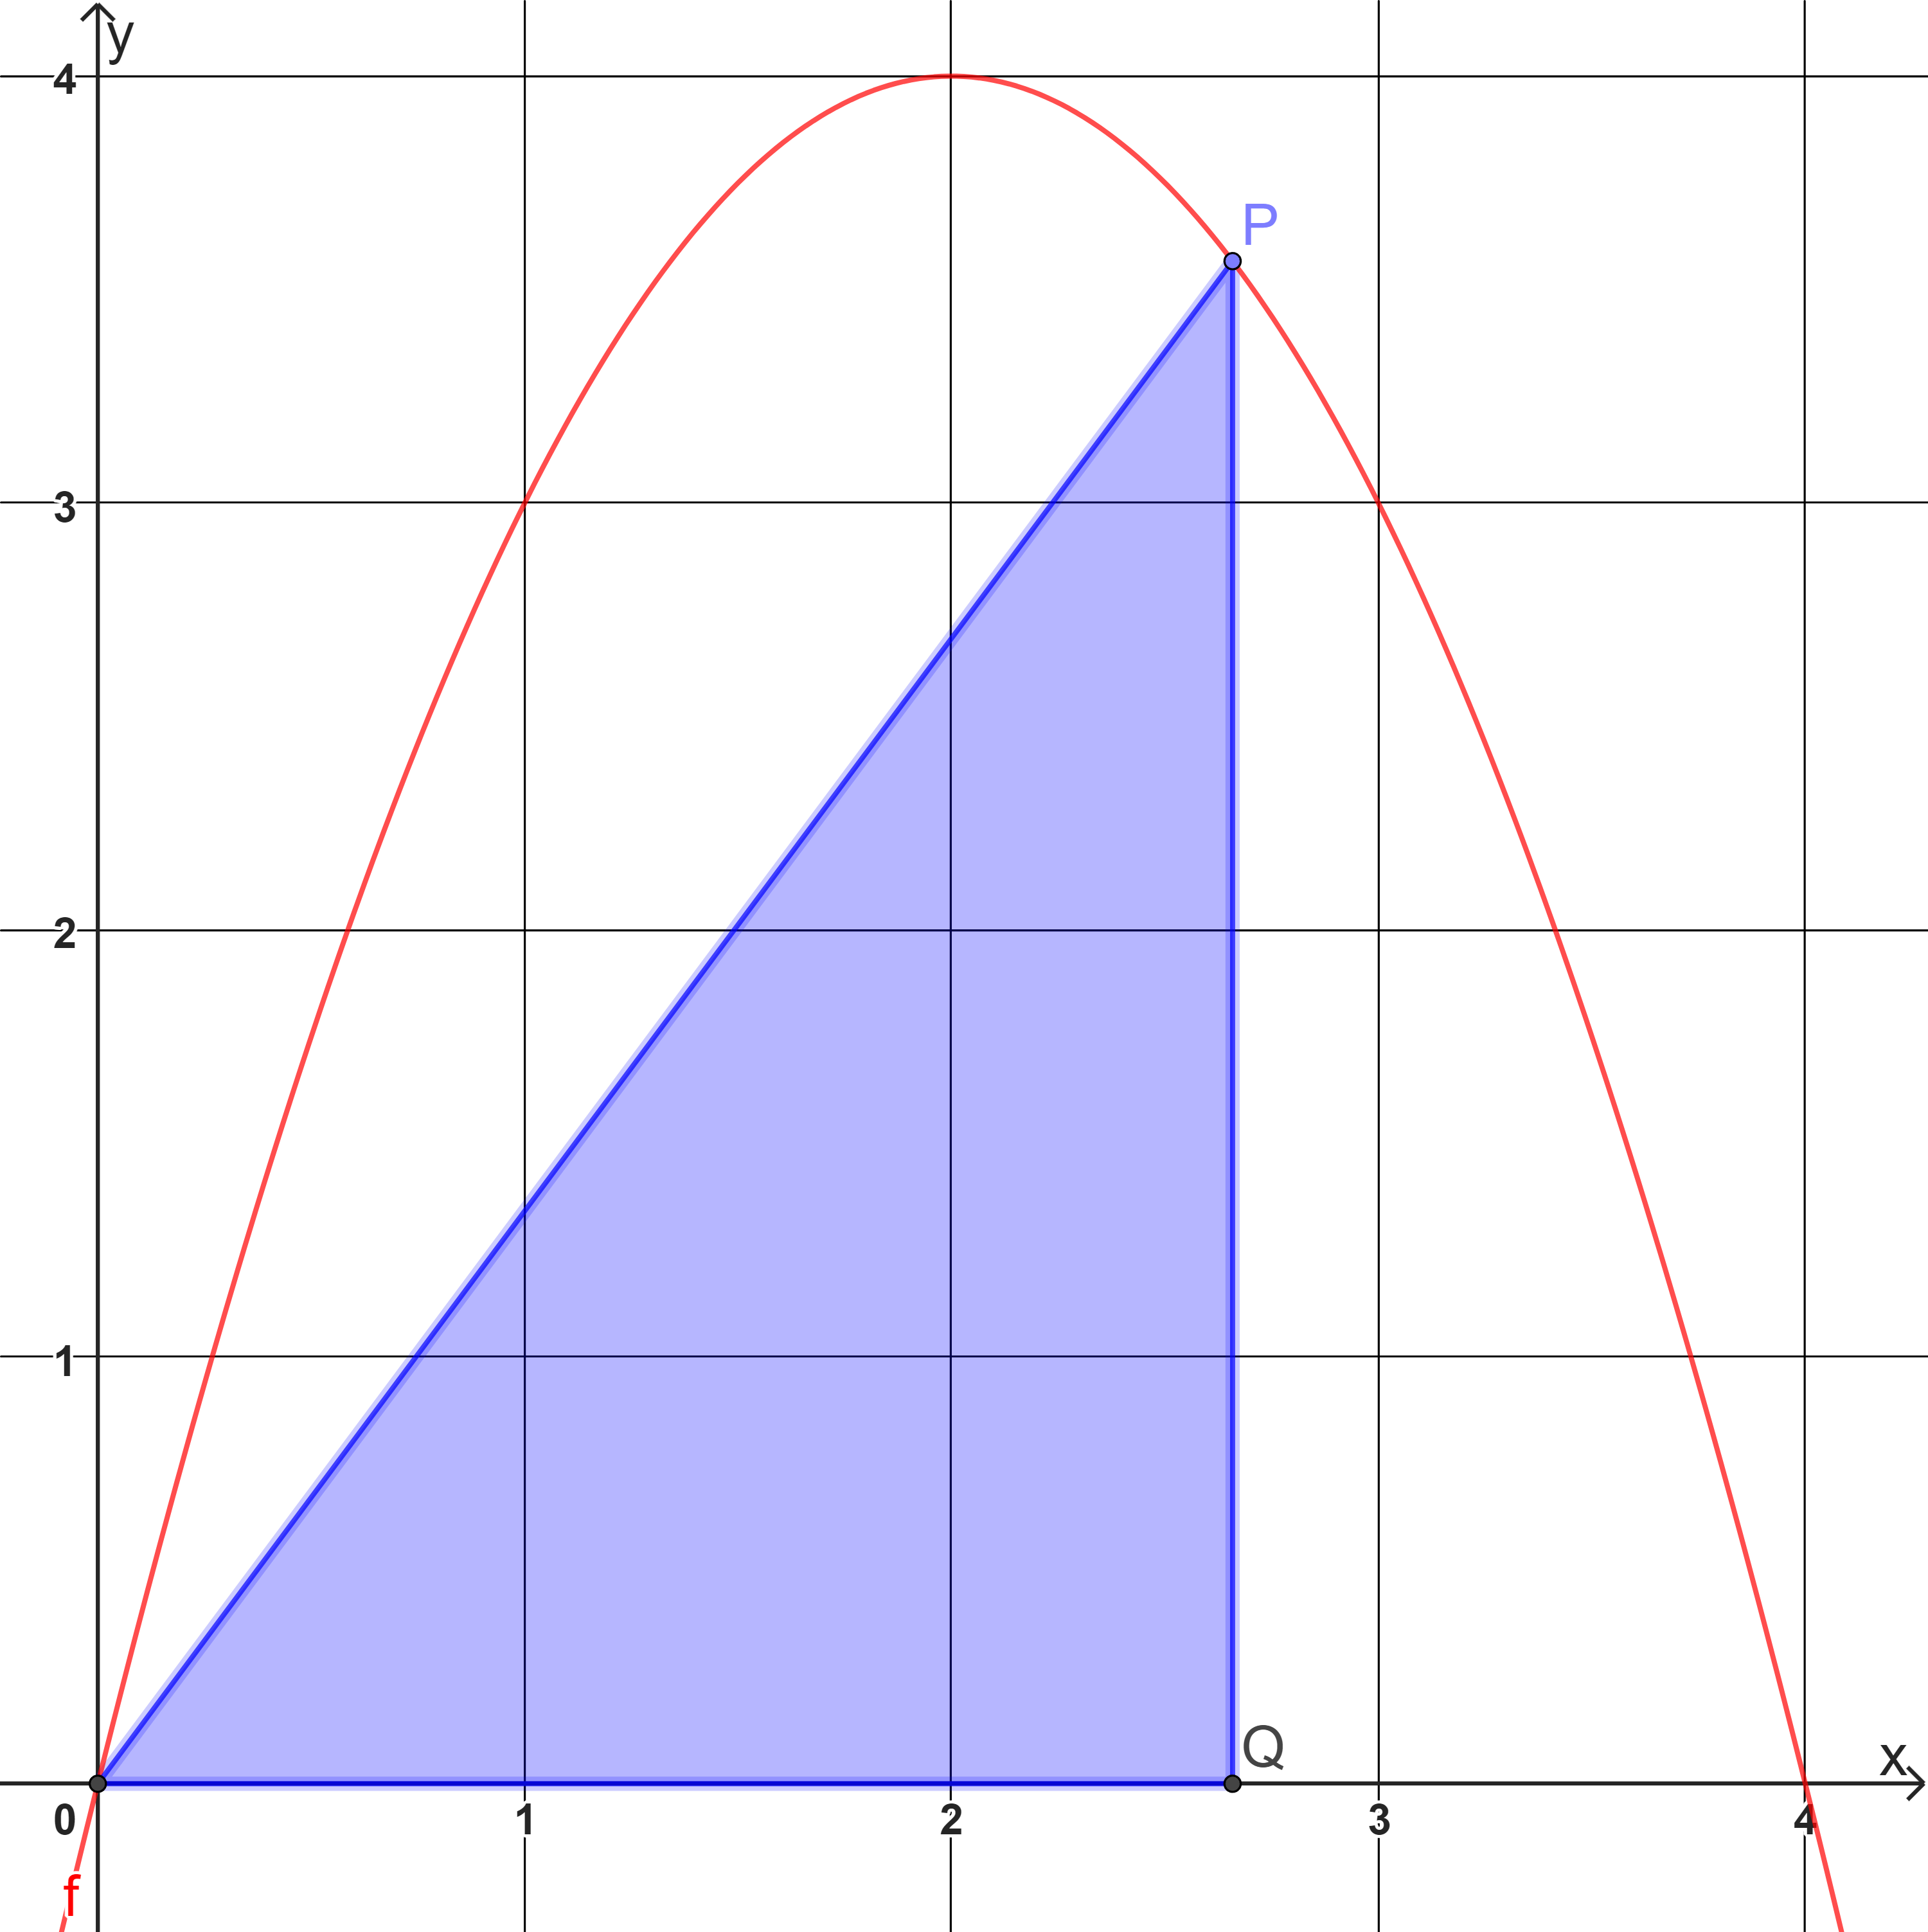
\includegraphics[width=\linewidth]{\optimierung/pics/Aufgabe_1.png}}%
		\end{minipage}}%
	\end{minipage}
\end{Answer}
%%%%%%%%%%%%%%%%%%%%%%%%%%%%%%%%%%%%%%%%%
\begin{Answer}[ref=optimierungA2]

    \bigskip

	\begin{minipage}{\textwidth}
		\adjustbox{valign=t}{\begin{minipage}{.5\textwidth}\raggedright
			\textbf{Zielfunktion}

			\(A(u)=2u\cdot f(u)=-2u^3+24u\) für \(0\leq u\leq \sqrt{12}\)

			Die Einschränkung für \(u\) ergibt sich aus der Tatsache, dass für negative \(u\) die Werte der Zielfunktion negativ werden und für \(u>\sqrt{12}\) liegt das Rechteck nicht mehr oberhalb der \(x\)-Achse.

			\textbf{Extremstellen der Zielfunktion}

			\(A'(u)=-6u^2+24\)

			\(A''(u)=-12u\)

			\(A'(u)=0\) liefert \(u_1=2\) und \(u_2=-2\). Dabei liegt \(u_2\) nicht mehr im erlaubten Bereich und kann ignoriert werden.

			Mit \(A''(2)=-24<0\) liegt bei \(u_1\) ein Hochpunkt.

			\textbf{Antwort erstellen}

			Der maximale Flächeninhalt beträgt \(A\left(2\right)=32\).

			Die Eckpunkte sind dann \(A(2\vert 0),\ B(2\vert f(2)=8),\ C(-2\vert 8),\ D(-2\vert 0)\).
		\end{minipage}}%
		\adjustbox{valign=t, padding = 2ex 0ex 0ex 0ex}{\begin{minipage}{.5\textwidth-2ex}                \iftoggle{qrcode}{
                    \settototalheight{\imgheight}{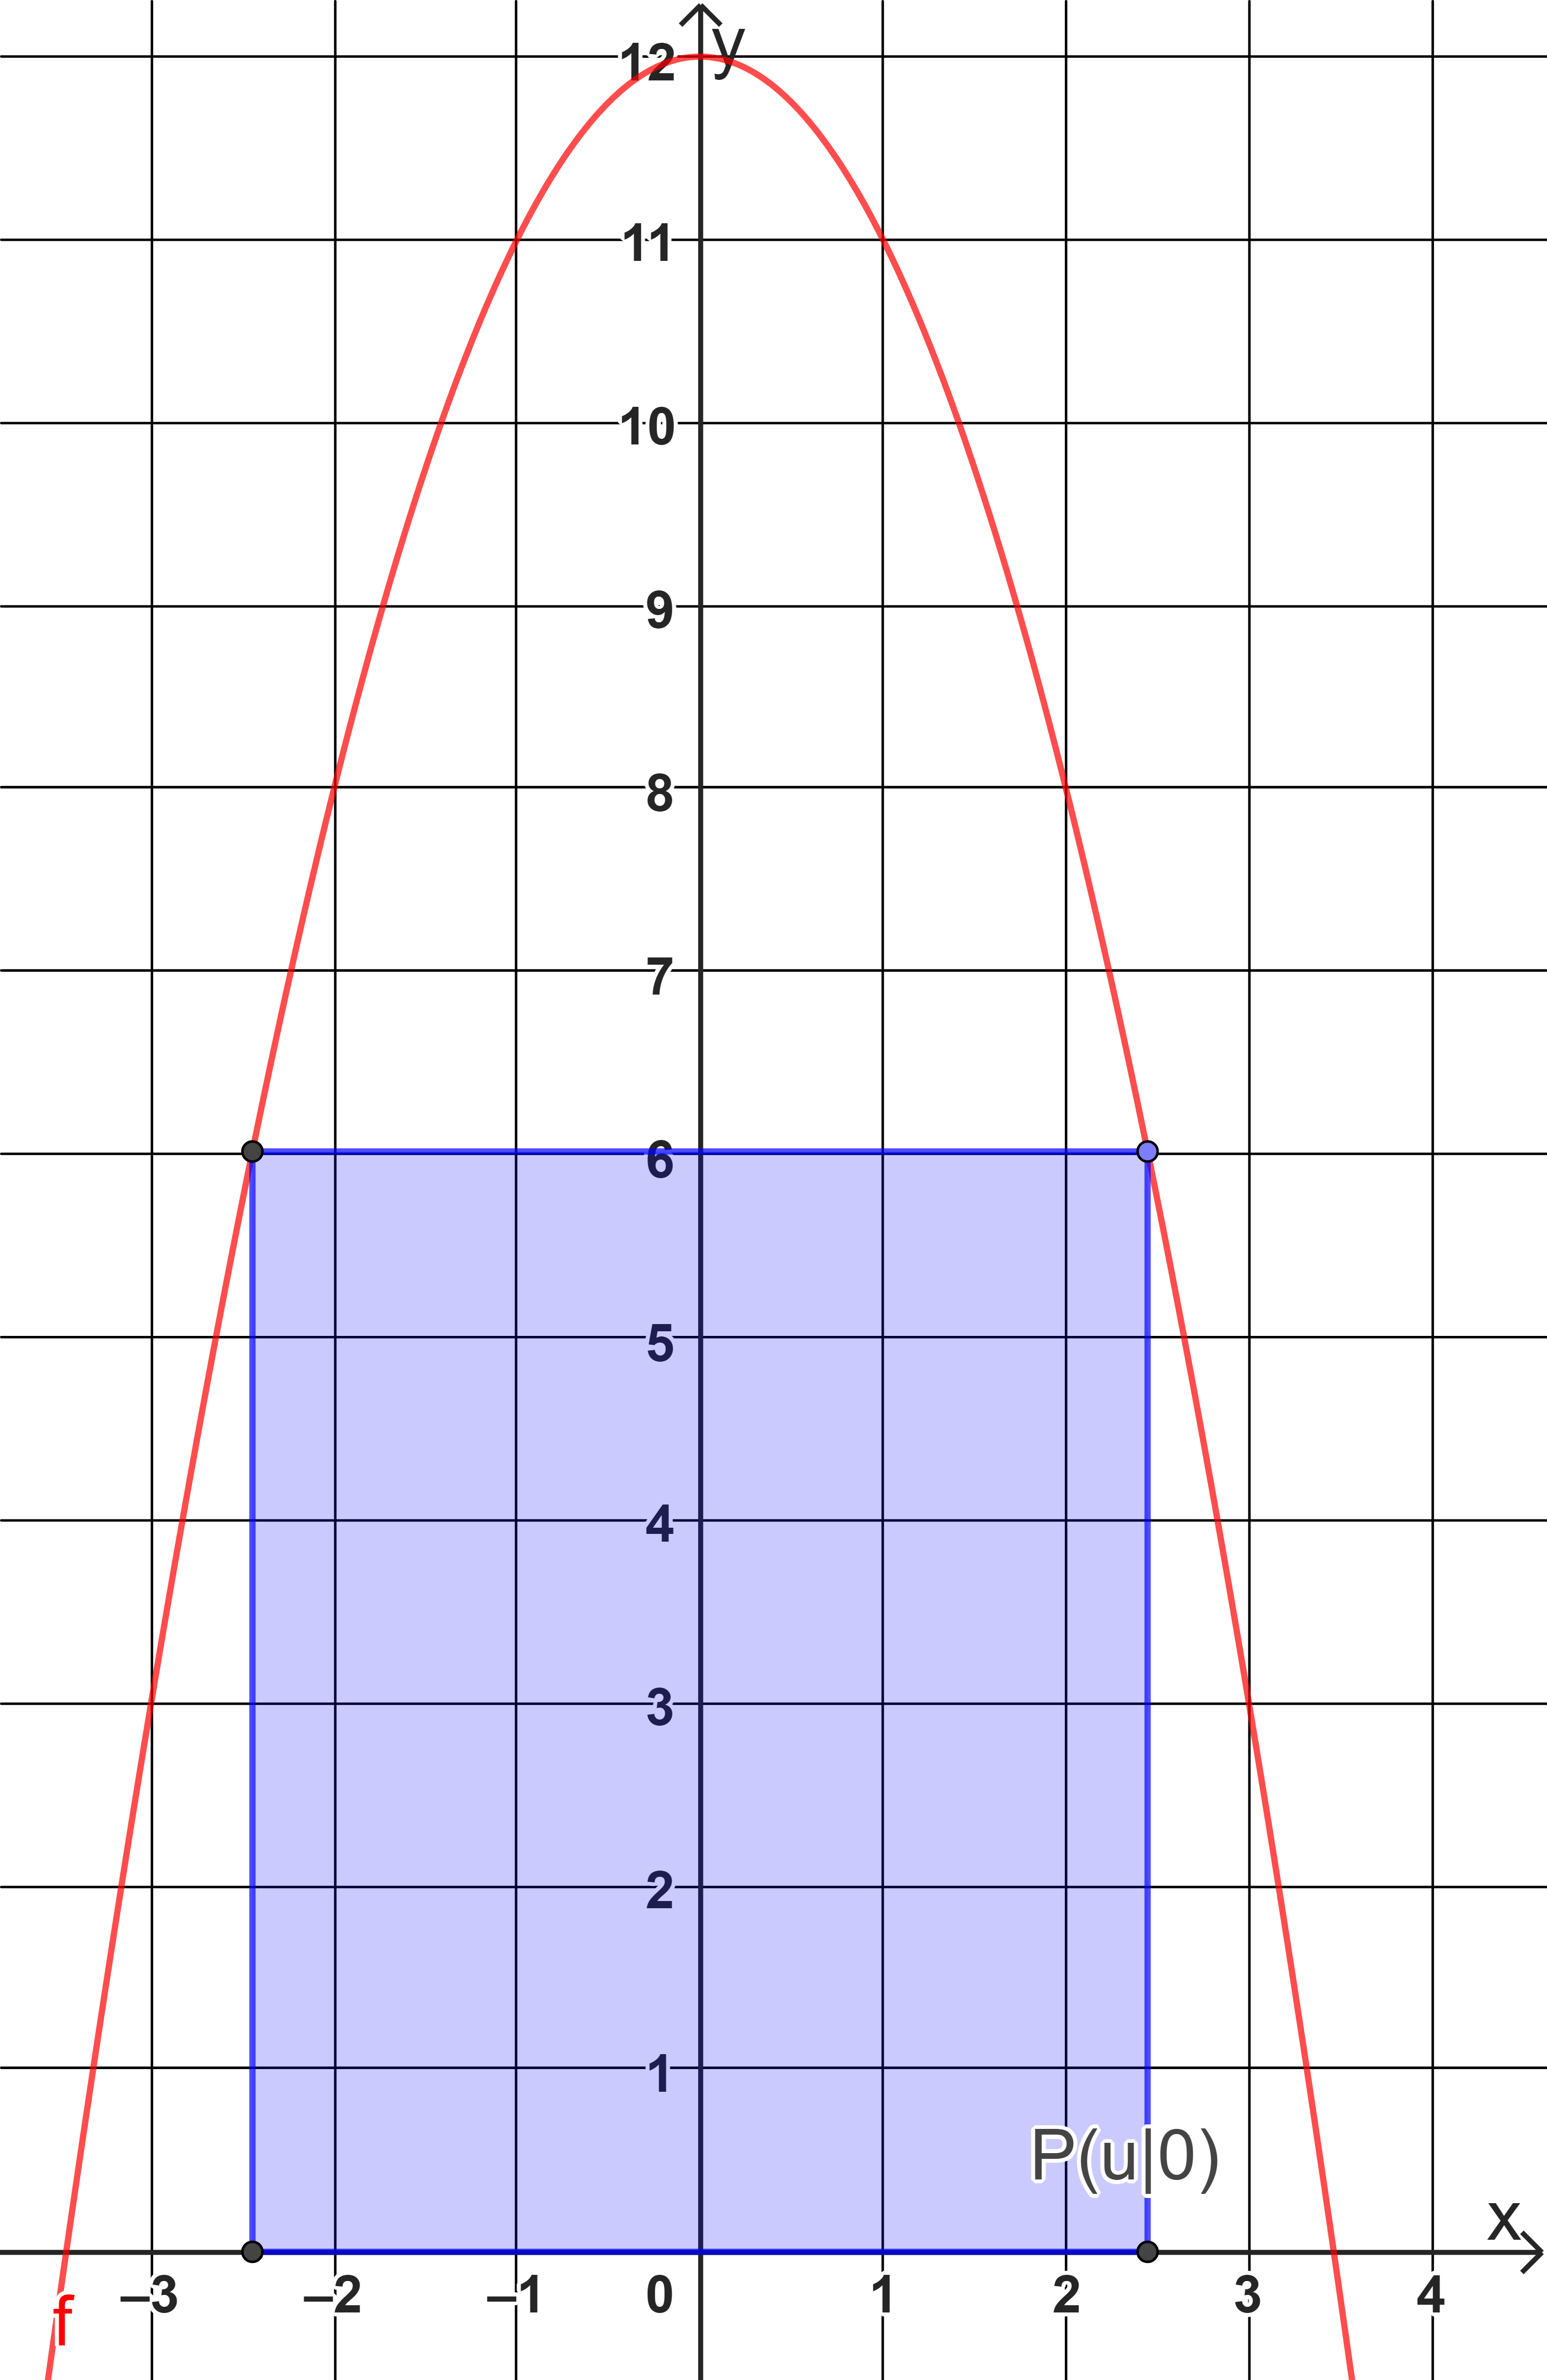
\includegraphics[width=\linewidth]{\optimierung/pics/Aufgabe_2.png}}%
                    \setlength{\qrheight}{2.5cm}%
                    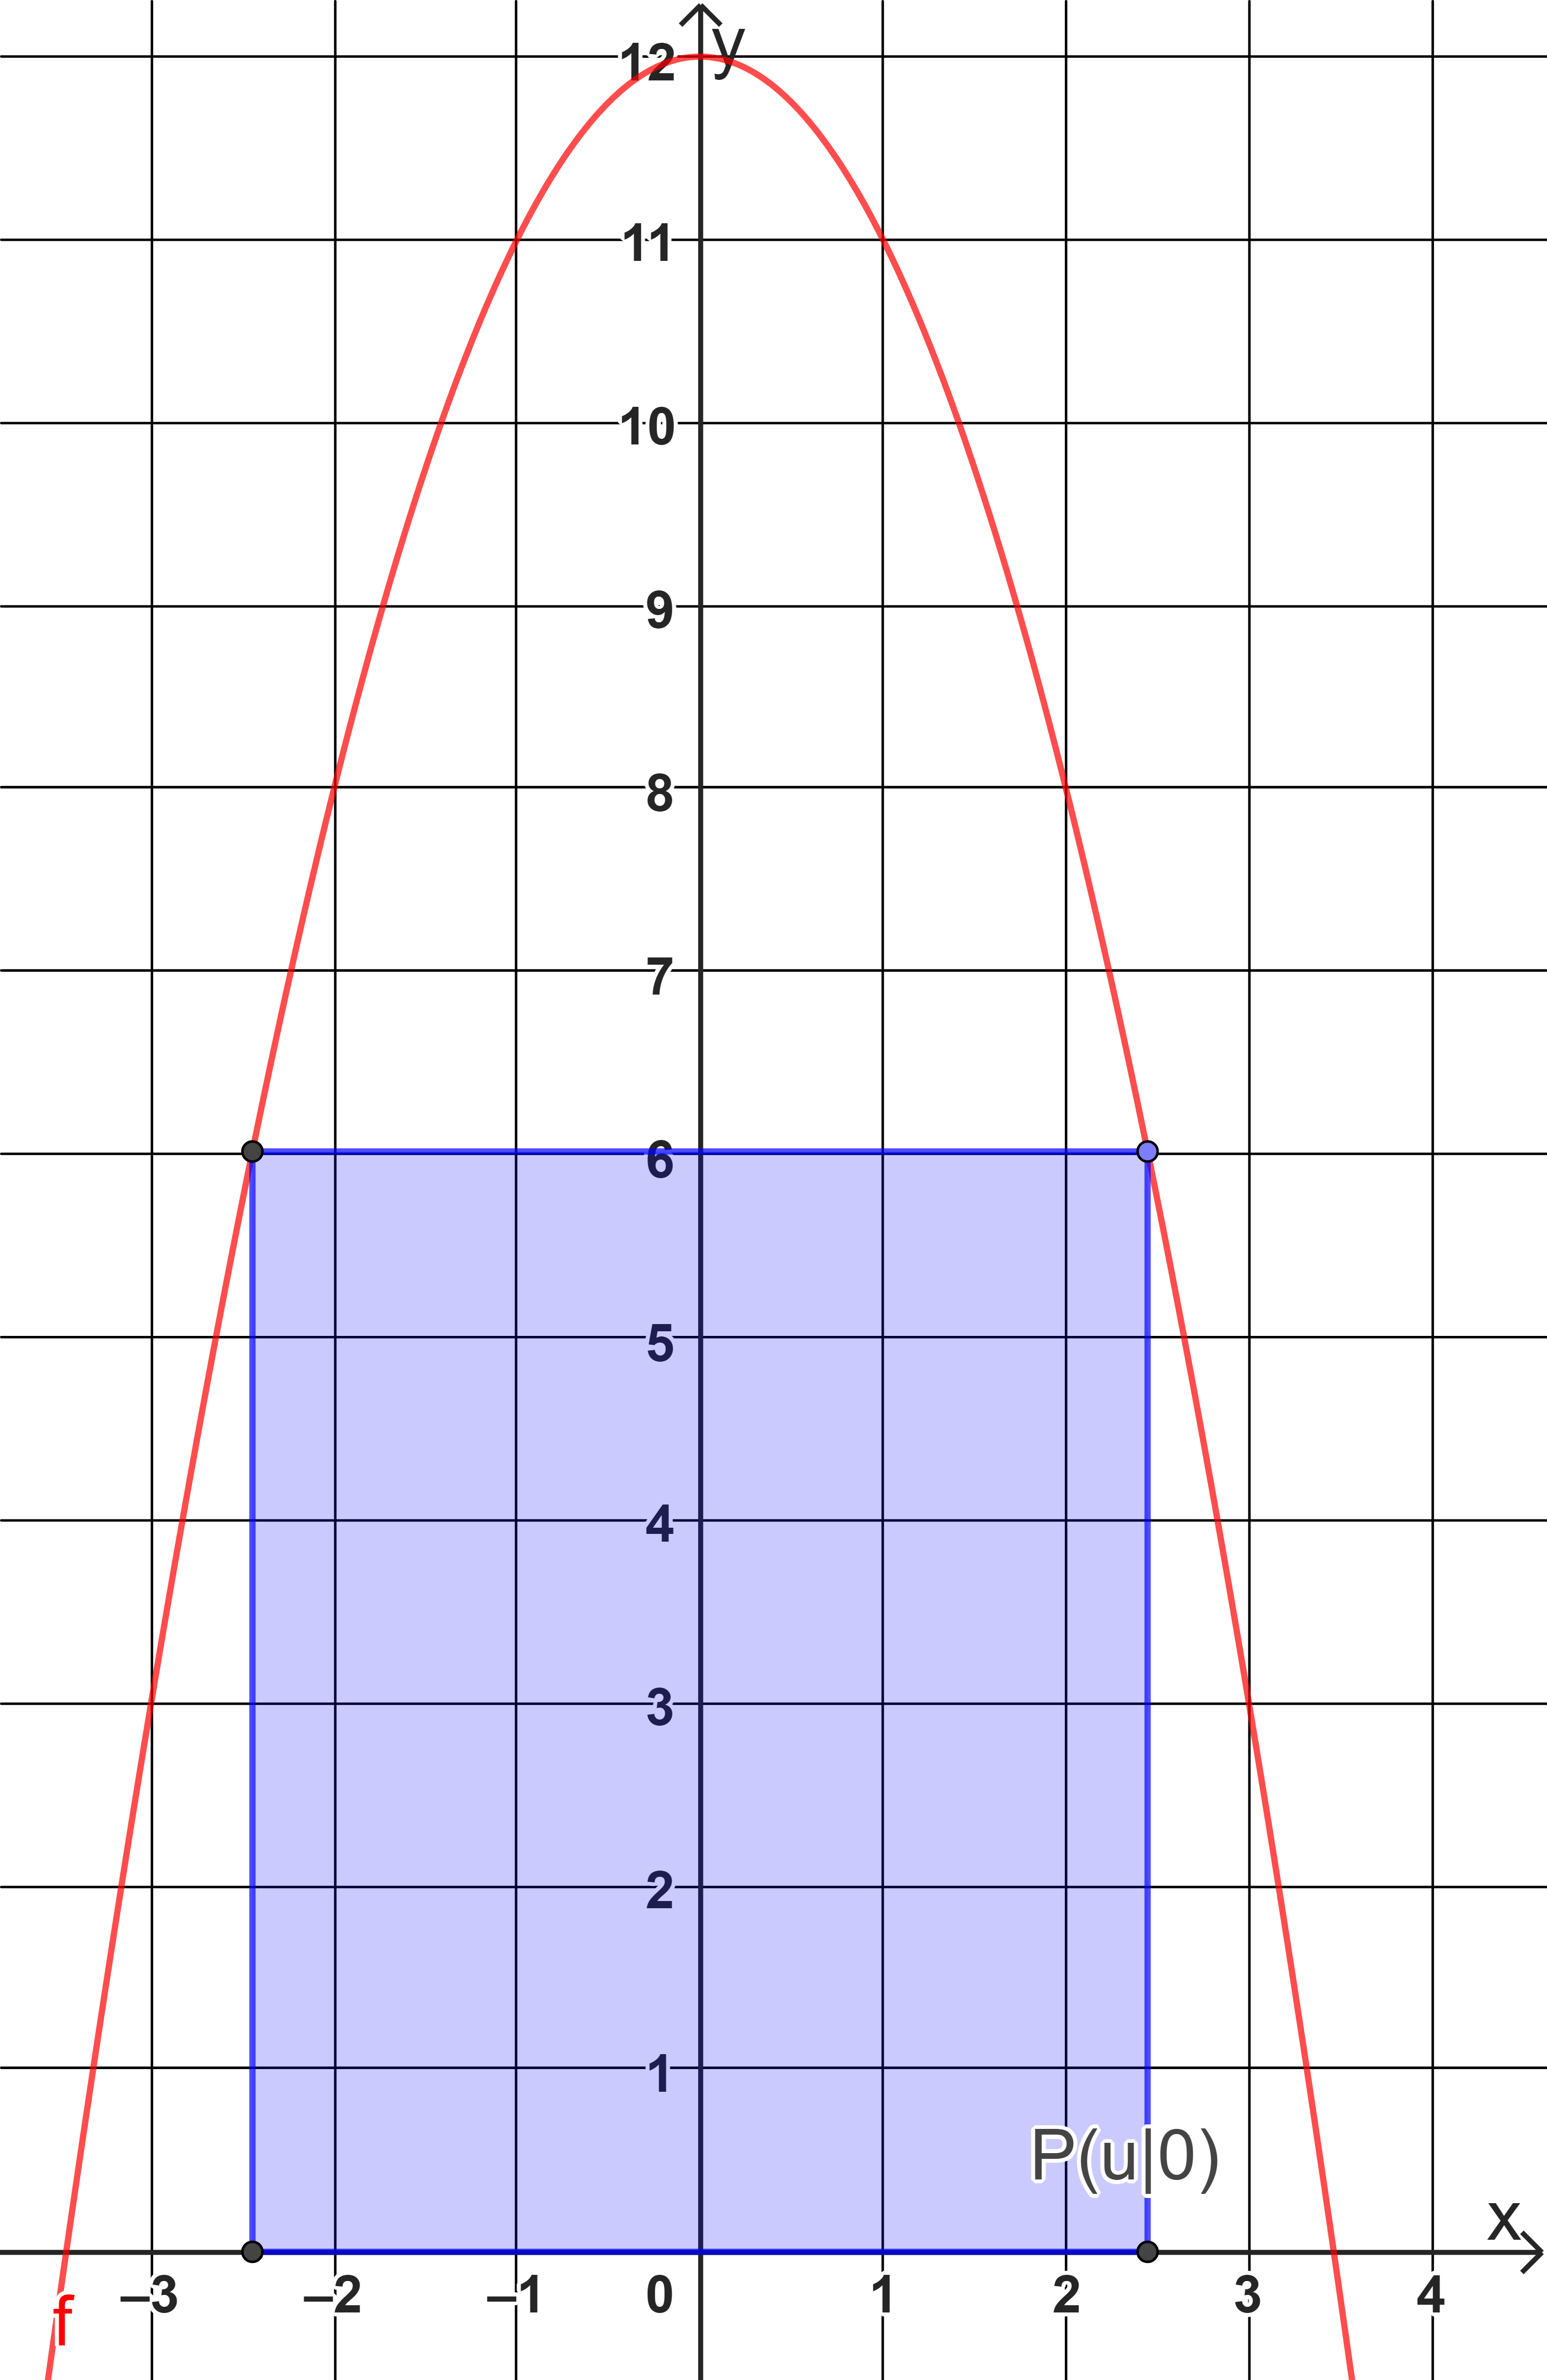
\includegraphics[width=\linewidth]{\optimierung/pics/Aufgabe_2.png}%
                    \raisebox{\imgheight-\qrheight}{\makebox[0pt][r]{\href{https://www.geogebra.org/m/bsju83ap}{
\includegraphics[height=\qrheight]{\optimierung/pics/Aufgabe_2QR.png}}}}%
                }{
                    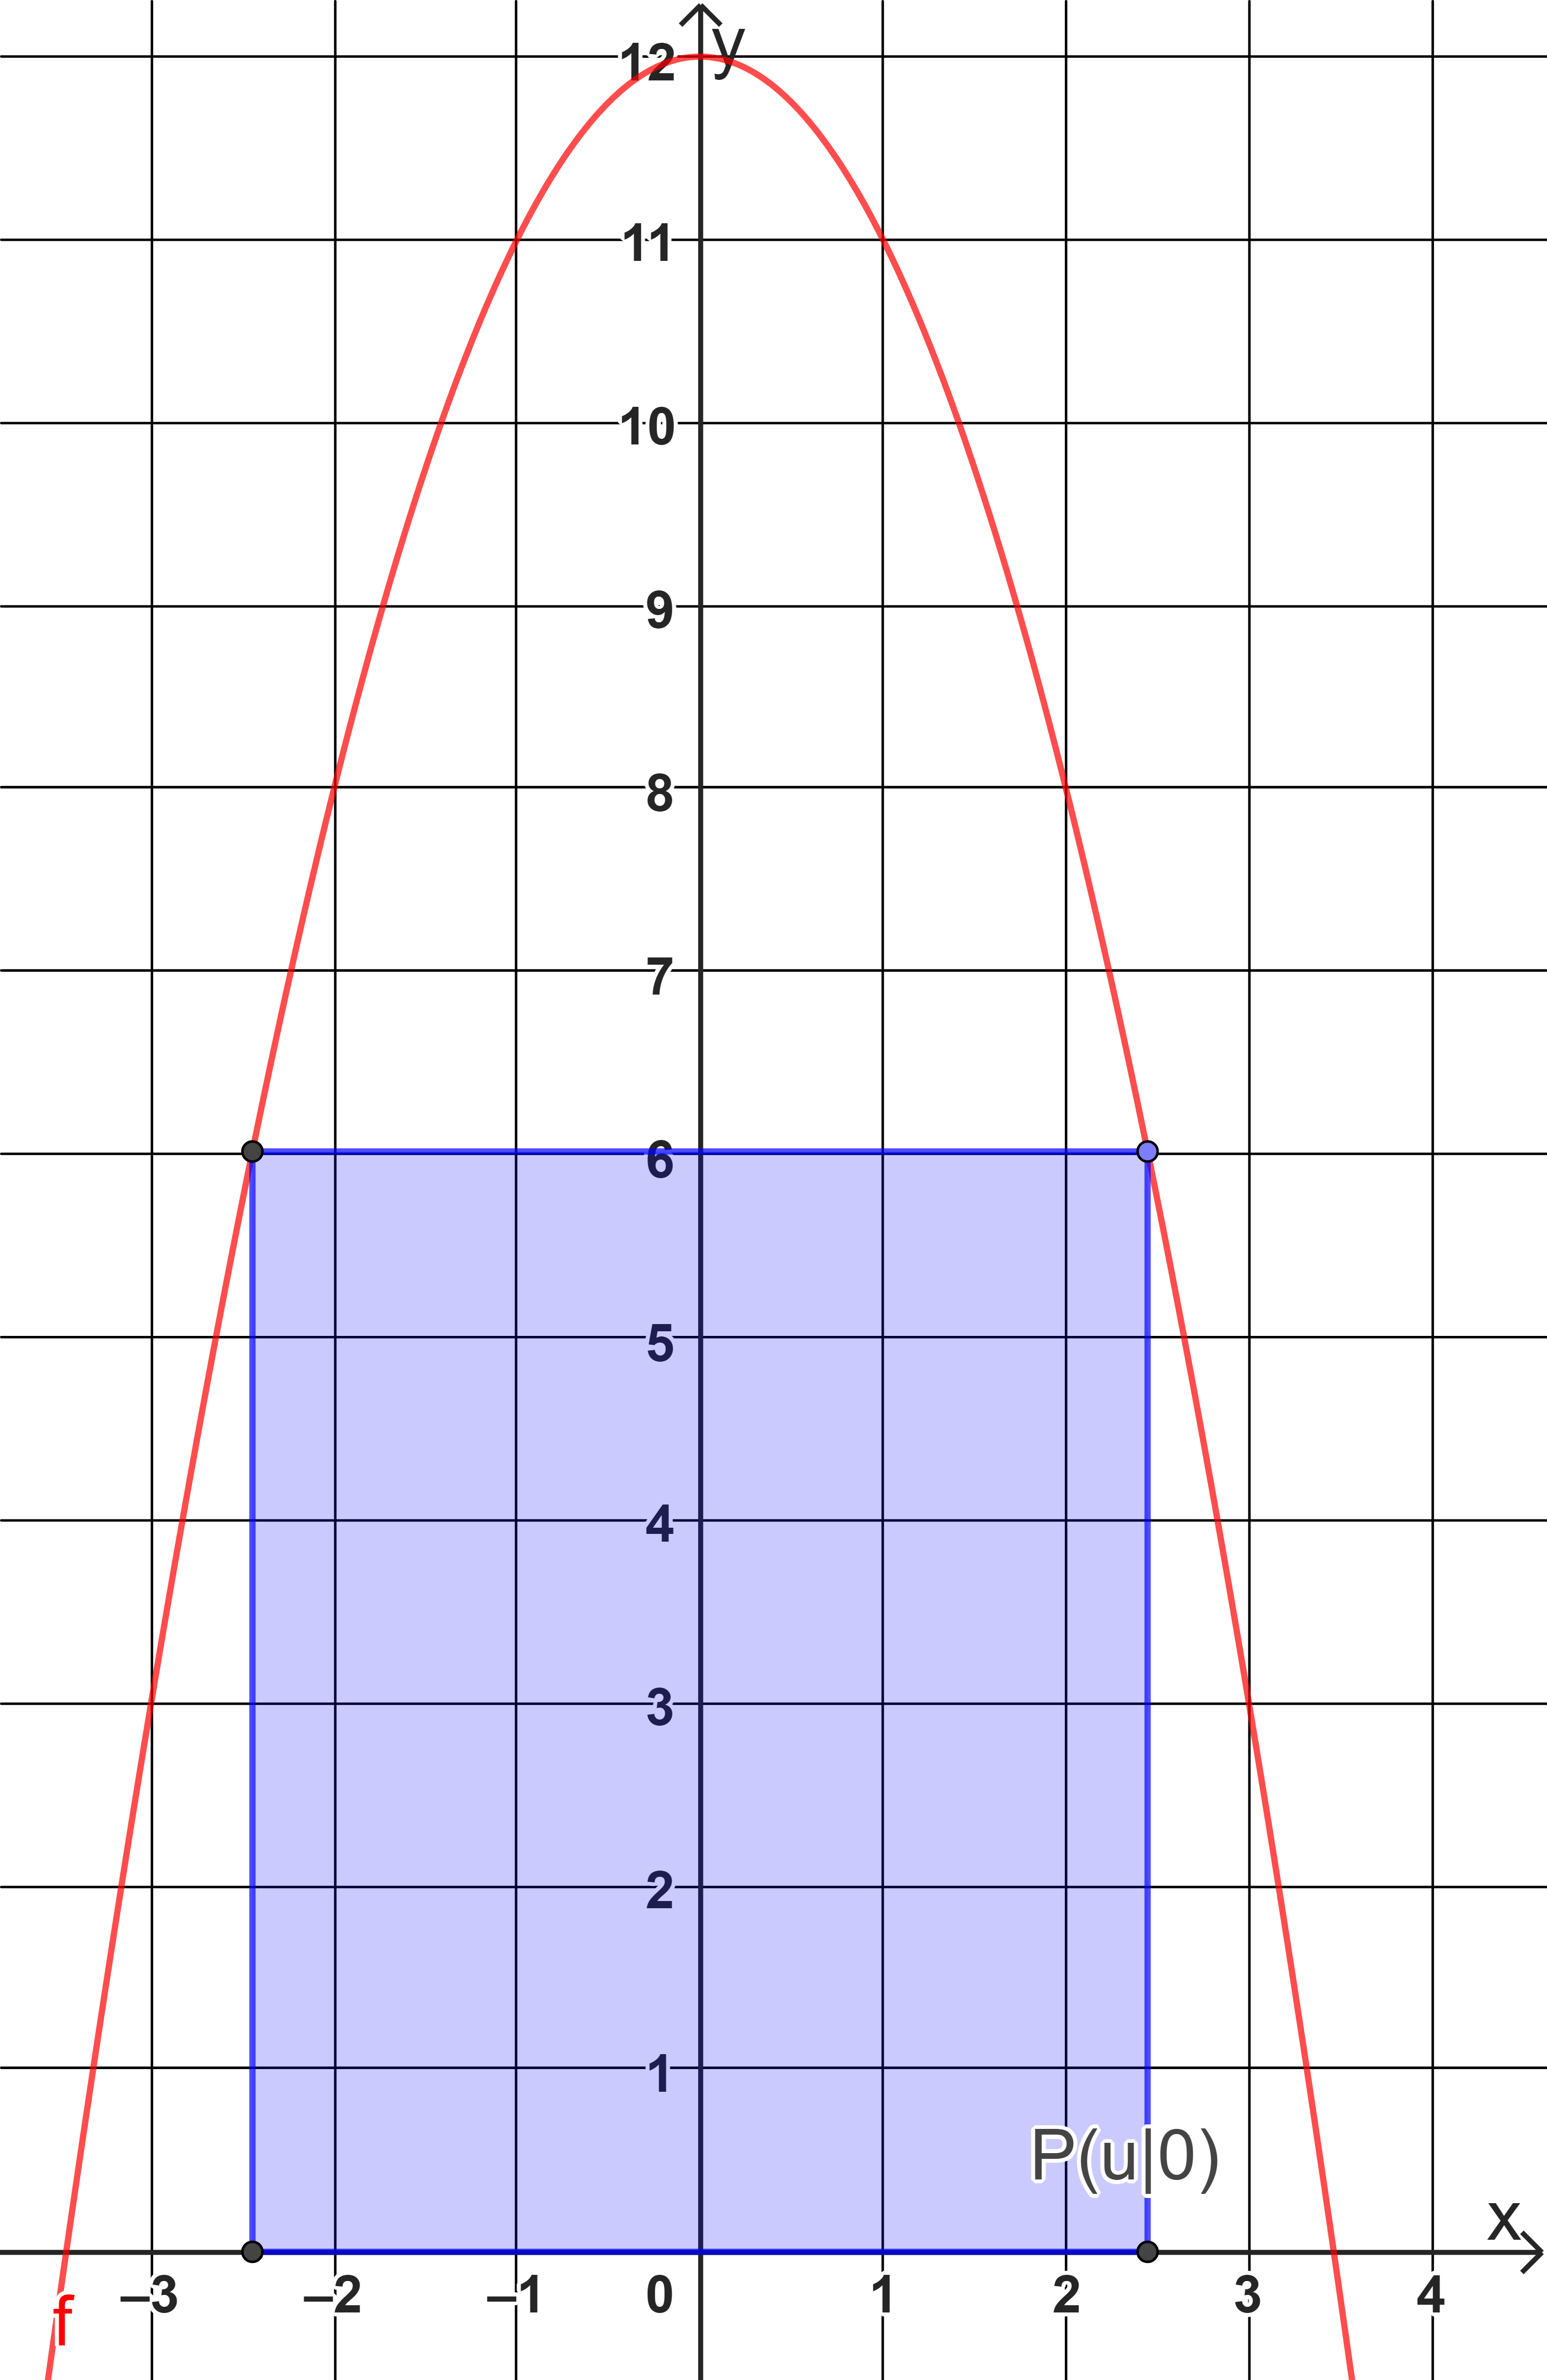
\includegraphics[width=\linewidth]{\optimierung/pics/Aufgabe_2.png}}%
        \end{minipage}}%
	\end{minipage}
\end{Answer}
%%%%%%%%%%%%%%%%%%%%%%%%%%%%%%%%%%%%%%%%%
\begin{Answer}[ref=optimierungA3]

    \bigskip

	\begin{minipage}{\textwidth}
		\adjustbox{valign=t}{\begin{minipage}{.5\textwidth}\raggedright
			\textbf{Zielfunktion}

			\(A(u)=2u\cdot \left(g(u)-f(u)\right)=-4u^3+12u\) für \(0\leq u\leq \sqrt{3}\)

			Die Einschränkung für \(u\) ergibt sich aus der Tatsache, dass für negative \(u\) die Werte der Zielfunktion negativ werden und für \(u>\sqrt{3}\) liegt das Rechteck nicht mehr zwischen den beiden Funktionen.

			\textbf{Extremstellen der Zielfunktion}

			\(A'(u)=-12u^2+12\)

			\(A''(u)=-24u\)

			\(A'(u)=0\) liefert \(u_1=1\) und \(u_2=-1\). Dabei liegt \(u_2\) nicht mehr im erlaubten Bereich und kann ignoriert werden.

			Mit \(A''(1)=-24<0\) liegt bei \(u_1\) ein Hochpunkt.

			\textbf{Antwort erstellen}

			Der maximale Flächeninhalt beträgt \(A\left(1\right)=8\).

			Die Eckpunkte sind dann\(A(1\vert f(1)=1),\)\\\(B(1\vert g(1)=5),\ C(-1\vert 5),\ D(-1\vert 1)\).
		\end{minipage}}%
        \adjustbox{valign=t, padding = 2ex 0ex 0ex 0ex}{\begin{minipage}{.5\textwidth-2ex}                \iftoggle{qrcode}{
            \settototalheight{\imgheight}{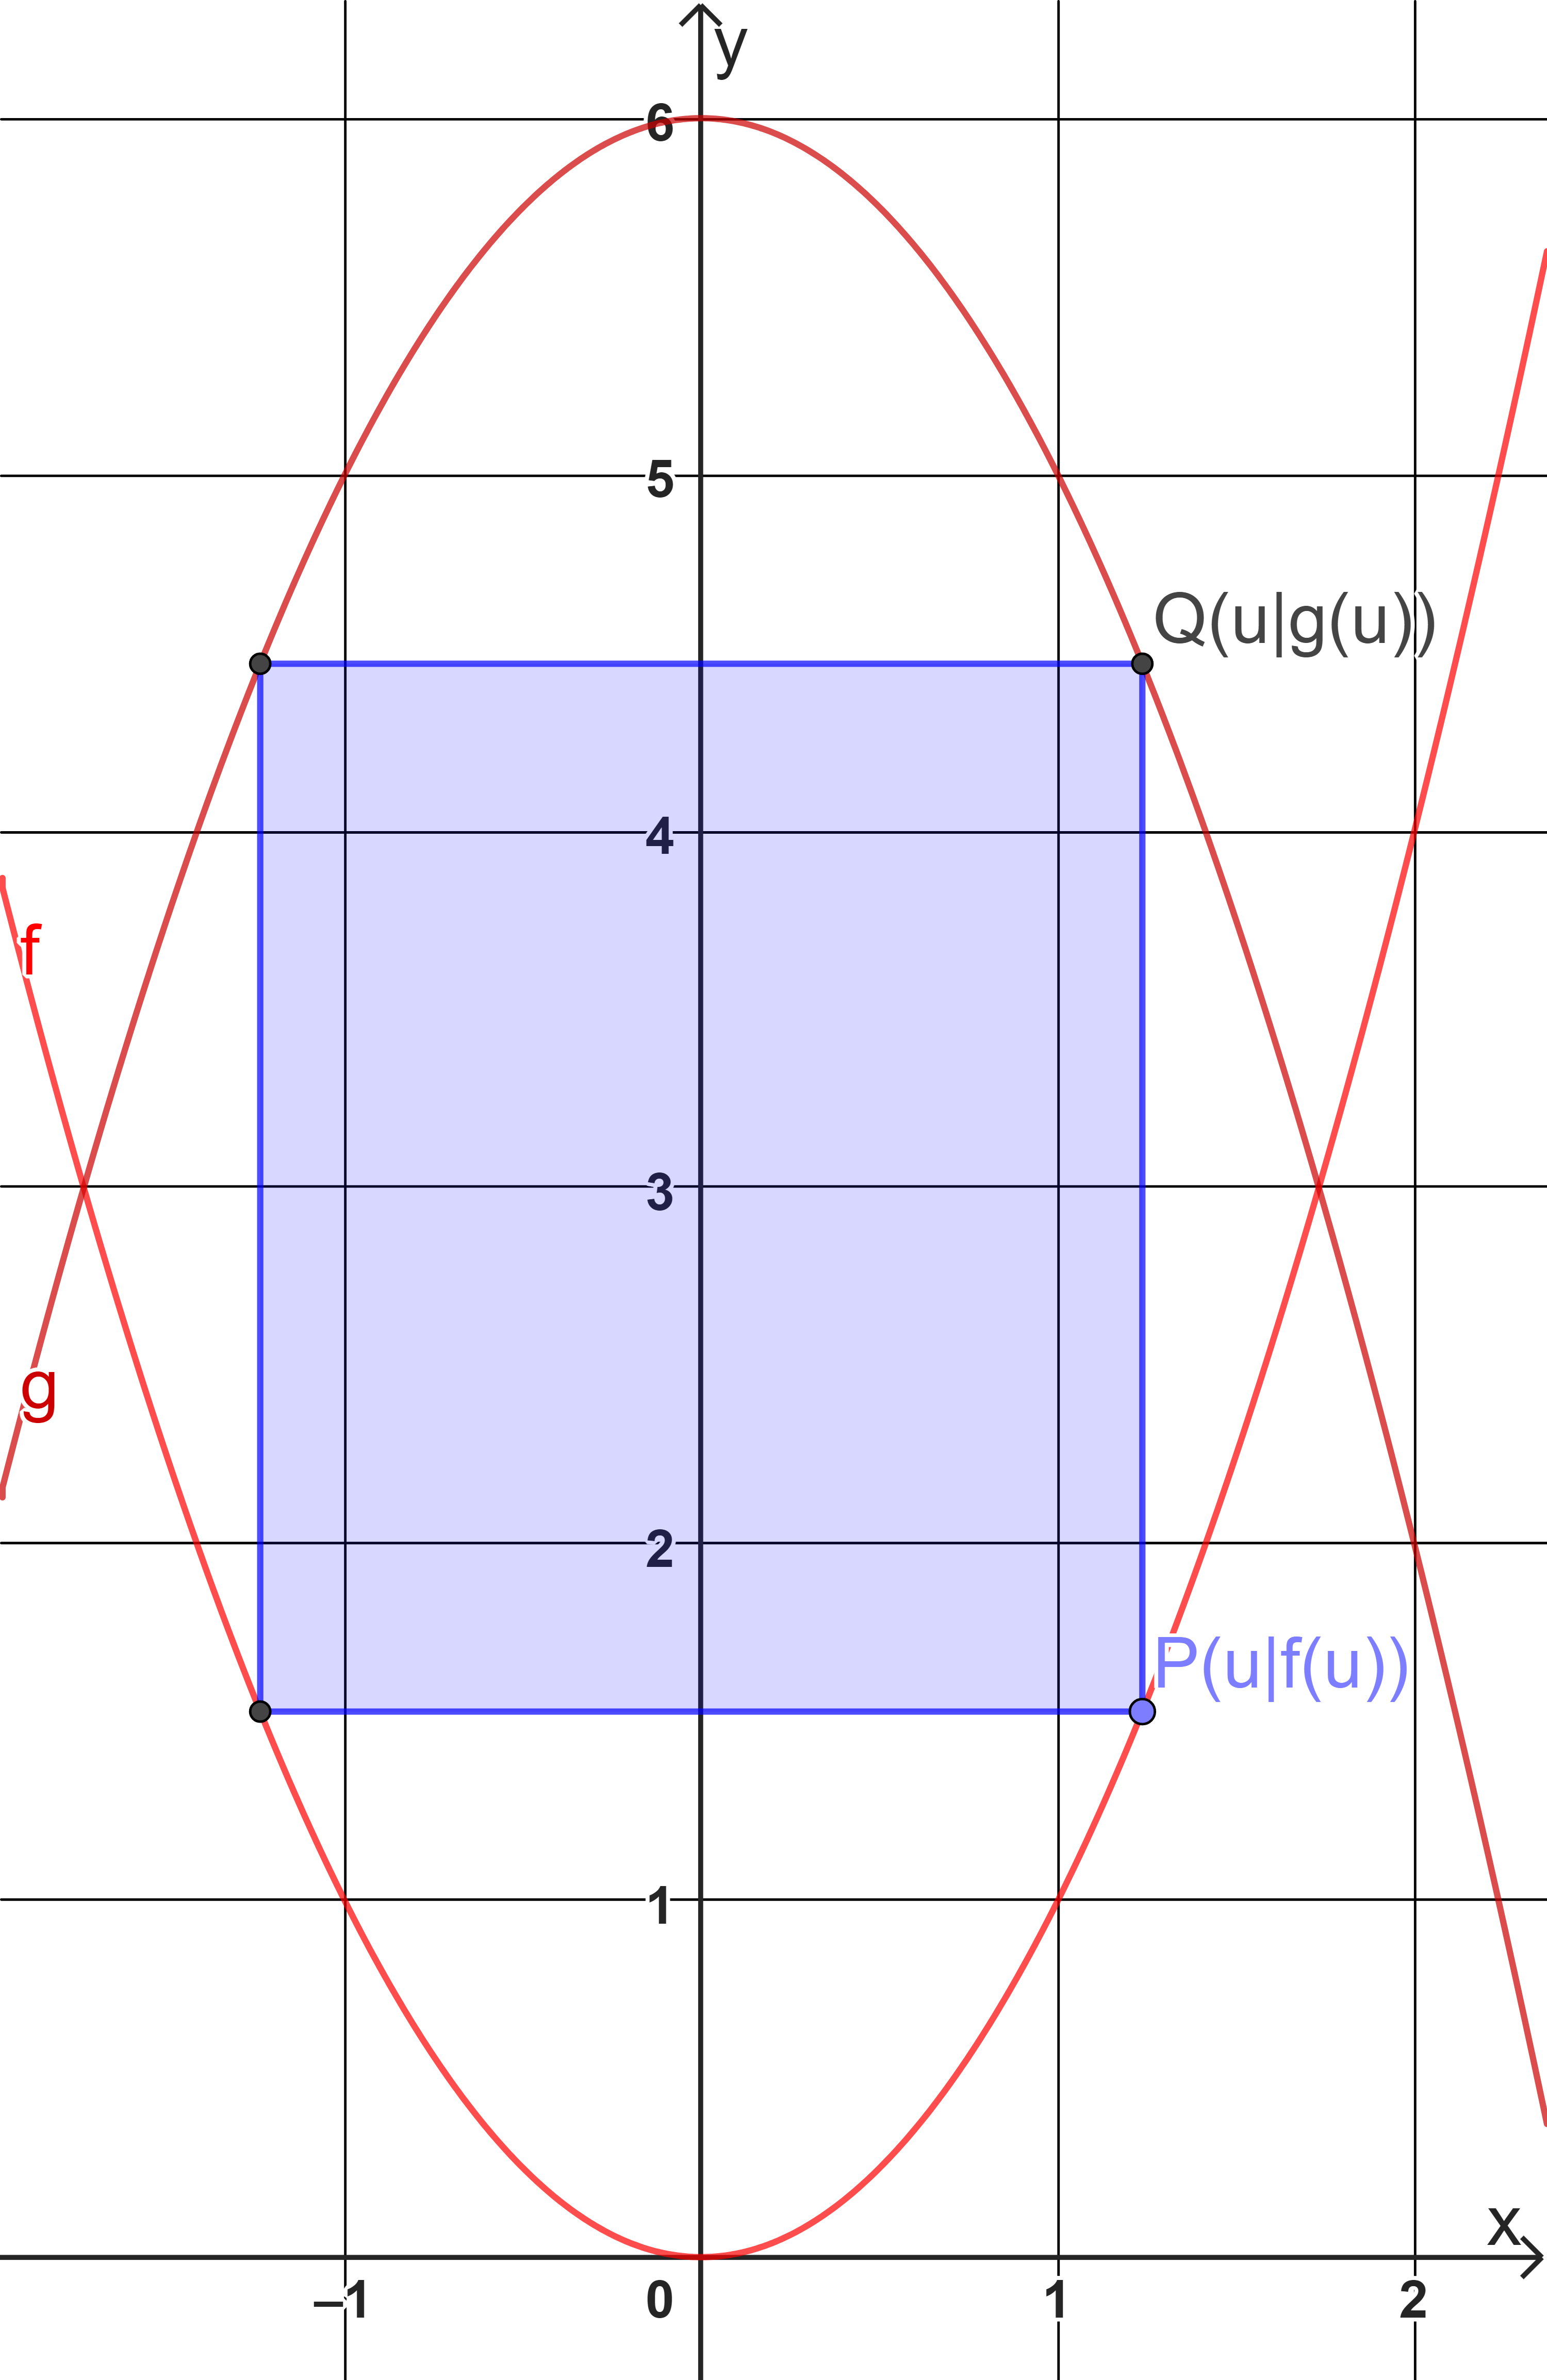
\includegraphics[width=\linewidth]{\optimierung/pics/Aufgabe_3.png}}%
            \setlength{\qrheight}{2.5cm}%
            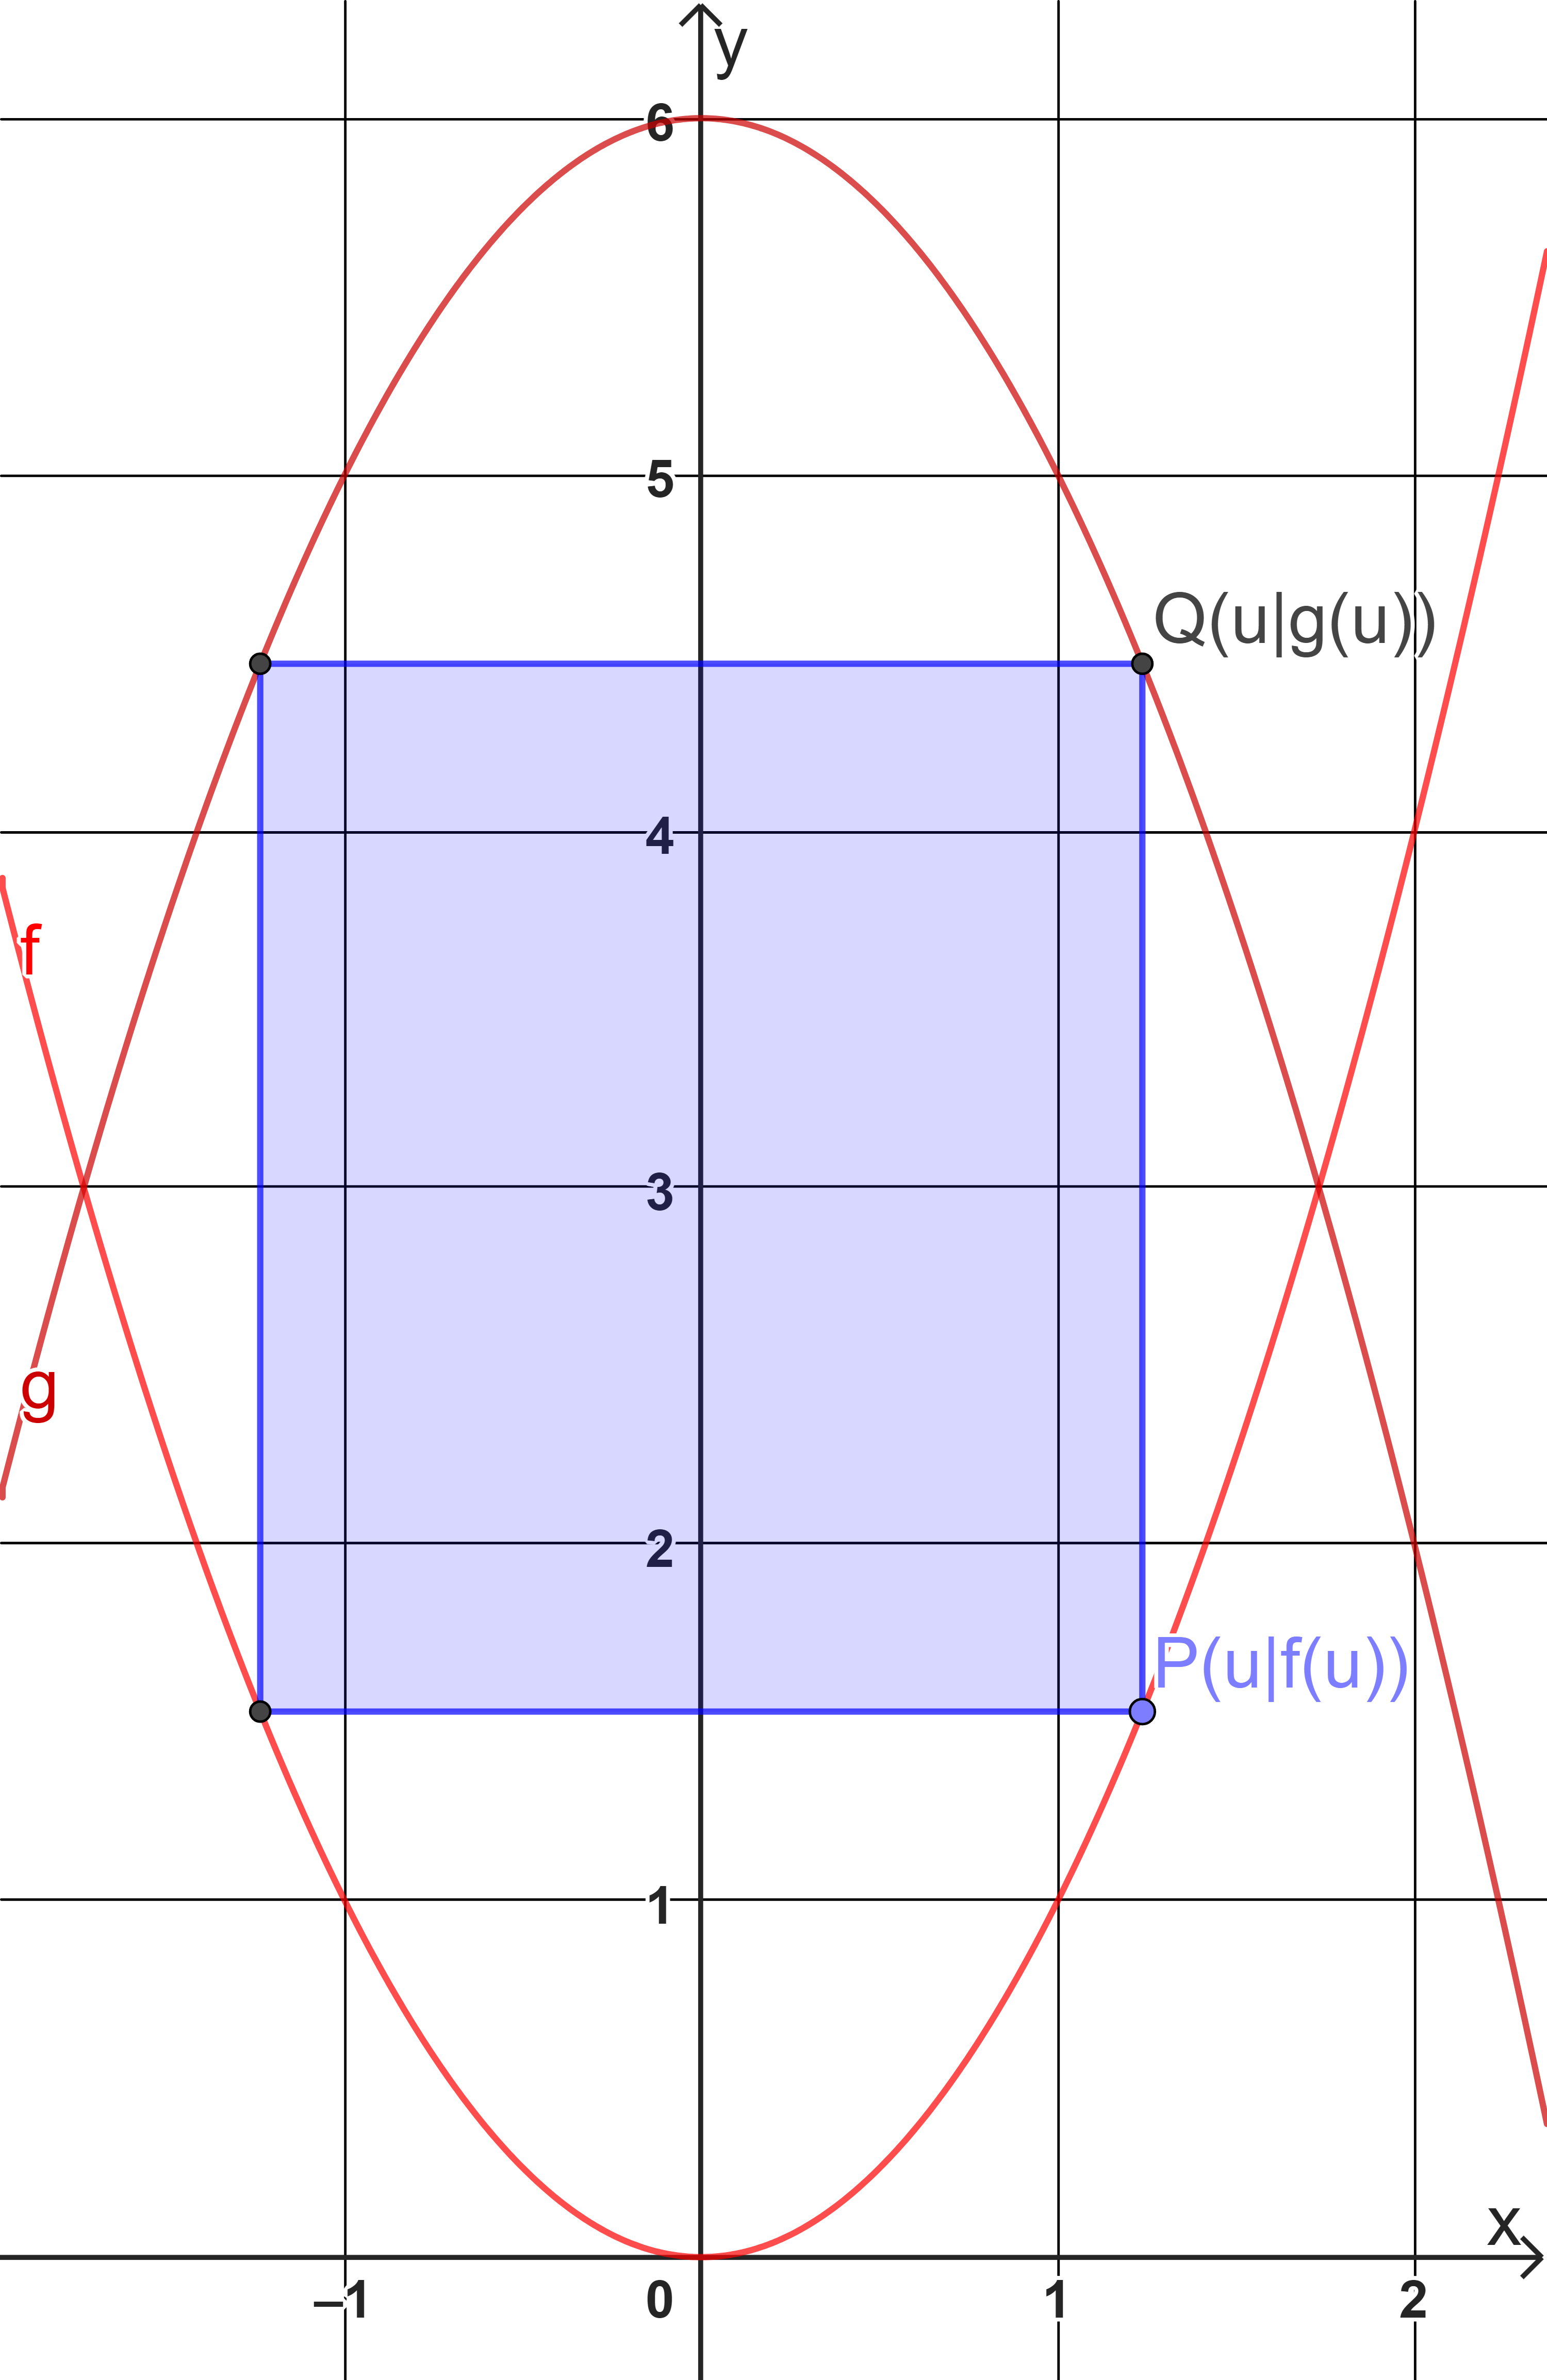
\includegraphics[width=\linewidth]{\optimierung/pics/Aufgabe_3.png}%
            \raisebox{\imgheight-\qrheight}{\makebox[0pt][r]{\href{https://www.geogebra.org/m/sq4gxae9}{
\includegraphics[height=\qrheight]{\optimierung/pics/Aufgabe_3QR.png}}}}%
        }{
            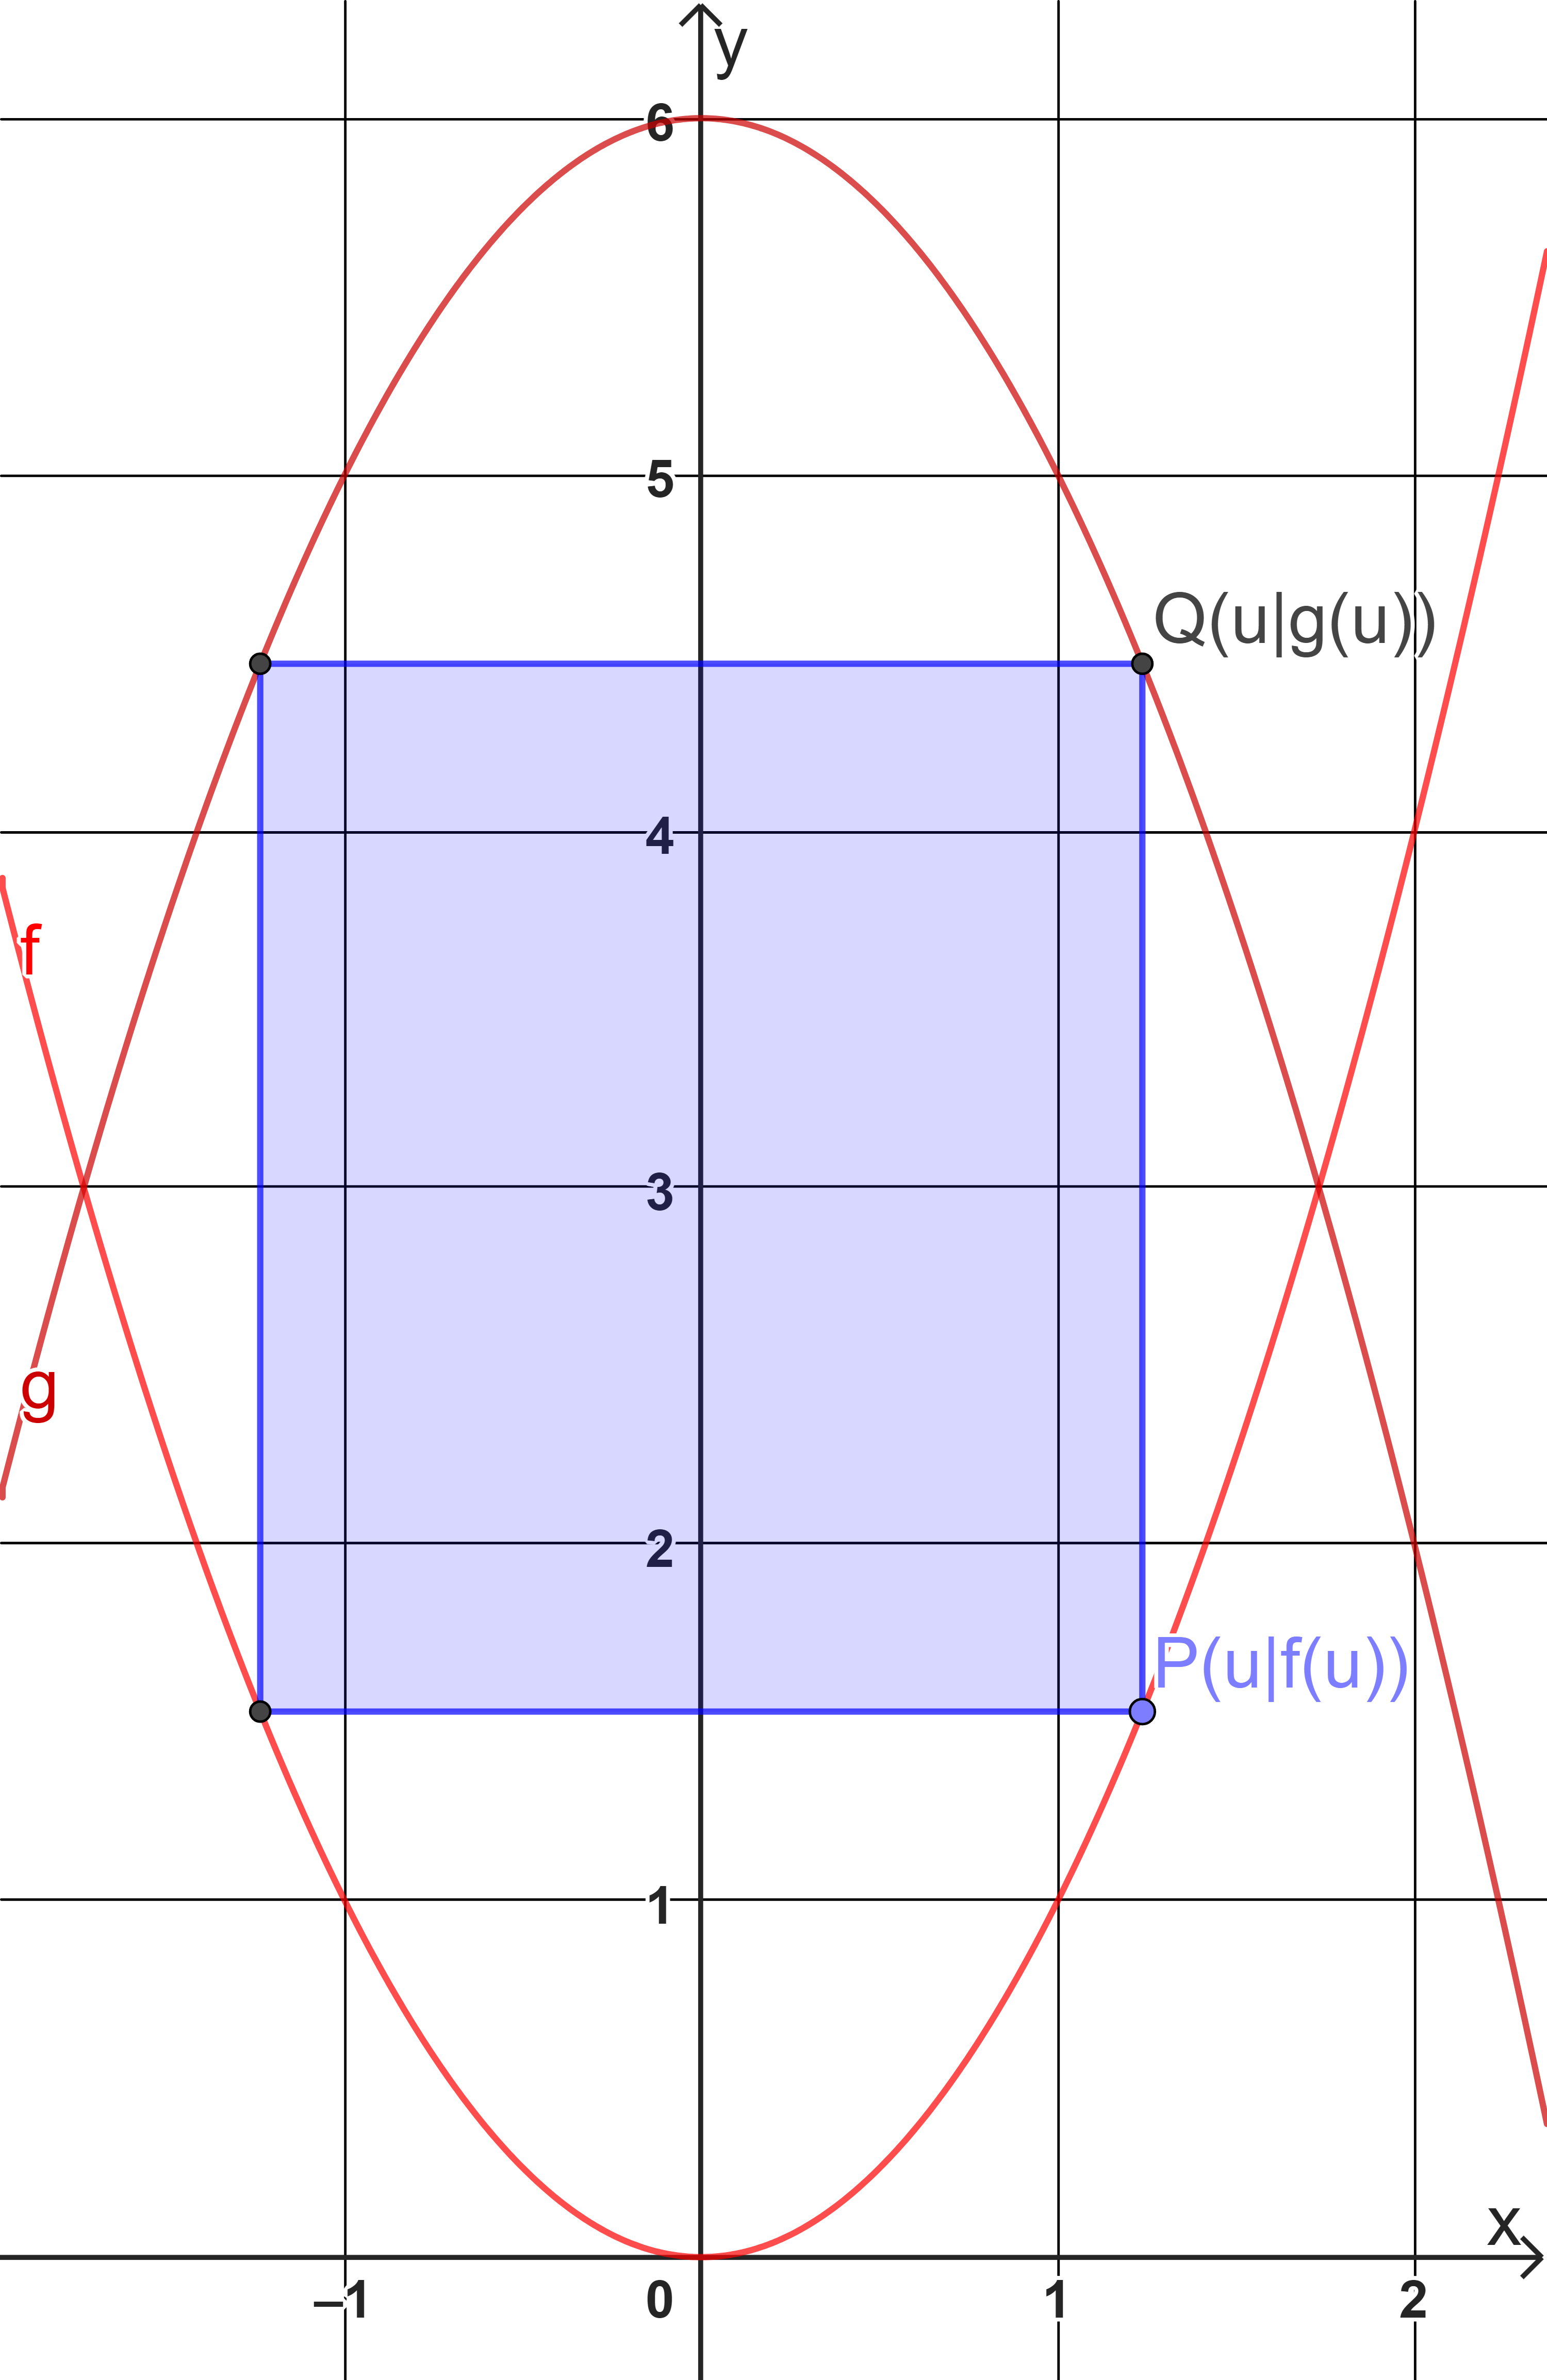
\includegraphics[width=\linewidth]{\optimierung/pics/Aufgabe_3.png}}%
    \end{minipage}}%
	\end{minipage}
\end{Answer}
%%%%%%%%%%%%%%%%%%%%%%%%%%%%%%%%%%%%%%%%%
\begin{Answer}[ref=optimierungA4]

    \bigskip

	\begin{minipage}{\textwidth}
		\adjustbox{valign=t}{\begin{minipage}{.5\textwidth}\raggedright
			\textbf{Zielfunktion}

			\(A(u)=u\cdot f(u)=u^3-6u^2+9u\)

			\textbf{Extremstellen der Zielfunktion}

			\(A'(u)=3u^2-12u+9\)

			\(A''(u)=6u-12\)

			\(A'(u)=0\) liefert \(u_1=3\) und \(u_2=1\).

			Mit \(A''(u_1)=6>0\) liegt bei \(u_1\) ein Tiefpunkt.

			Mit \(A''(u_2)=-6<0\) liegt bei \(u_2\) ein Hochpunkt.

			\textbf{Antwort erstellen}

			Der maximale Flächeninhalt beträgt \(A\left(u_2\right)=4\).

			Die Eckpunkte sind dann
			\(A\left(0\vert 0\right),
			\ B\left(1\middle\vert 0\right),\newline
			\ C\left(1\middle\vert f(u_2)=4\right),\ D\left(0\middle\vert 4\right)\).
		\end{minipage}}%
        \adjustbox{valign=t, padding = 2ex 0ex 0ex 0ex}{\begin{minipage}{.5\textwidth-2ex}                \iftoggle{qrcode}{
            \settototalheight{\imgheight}{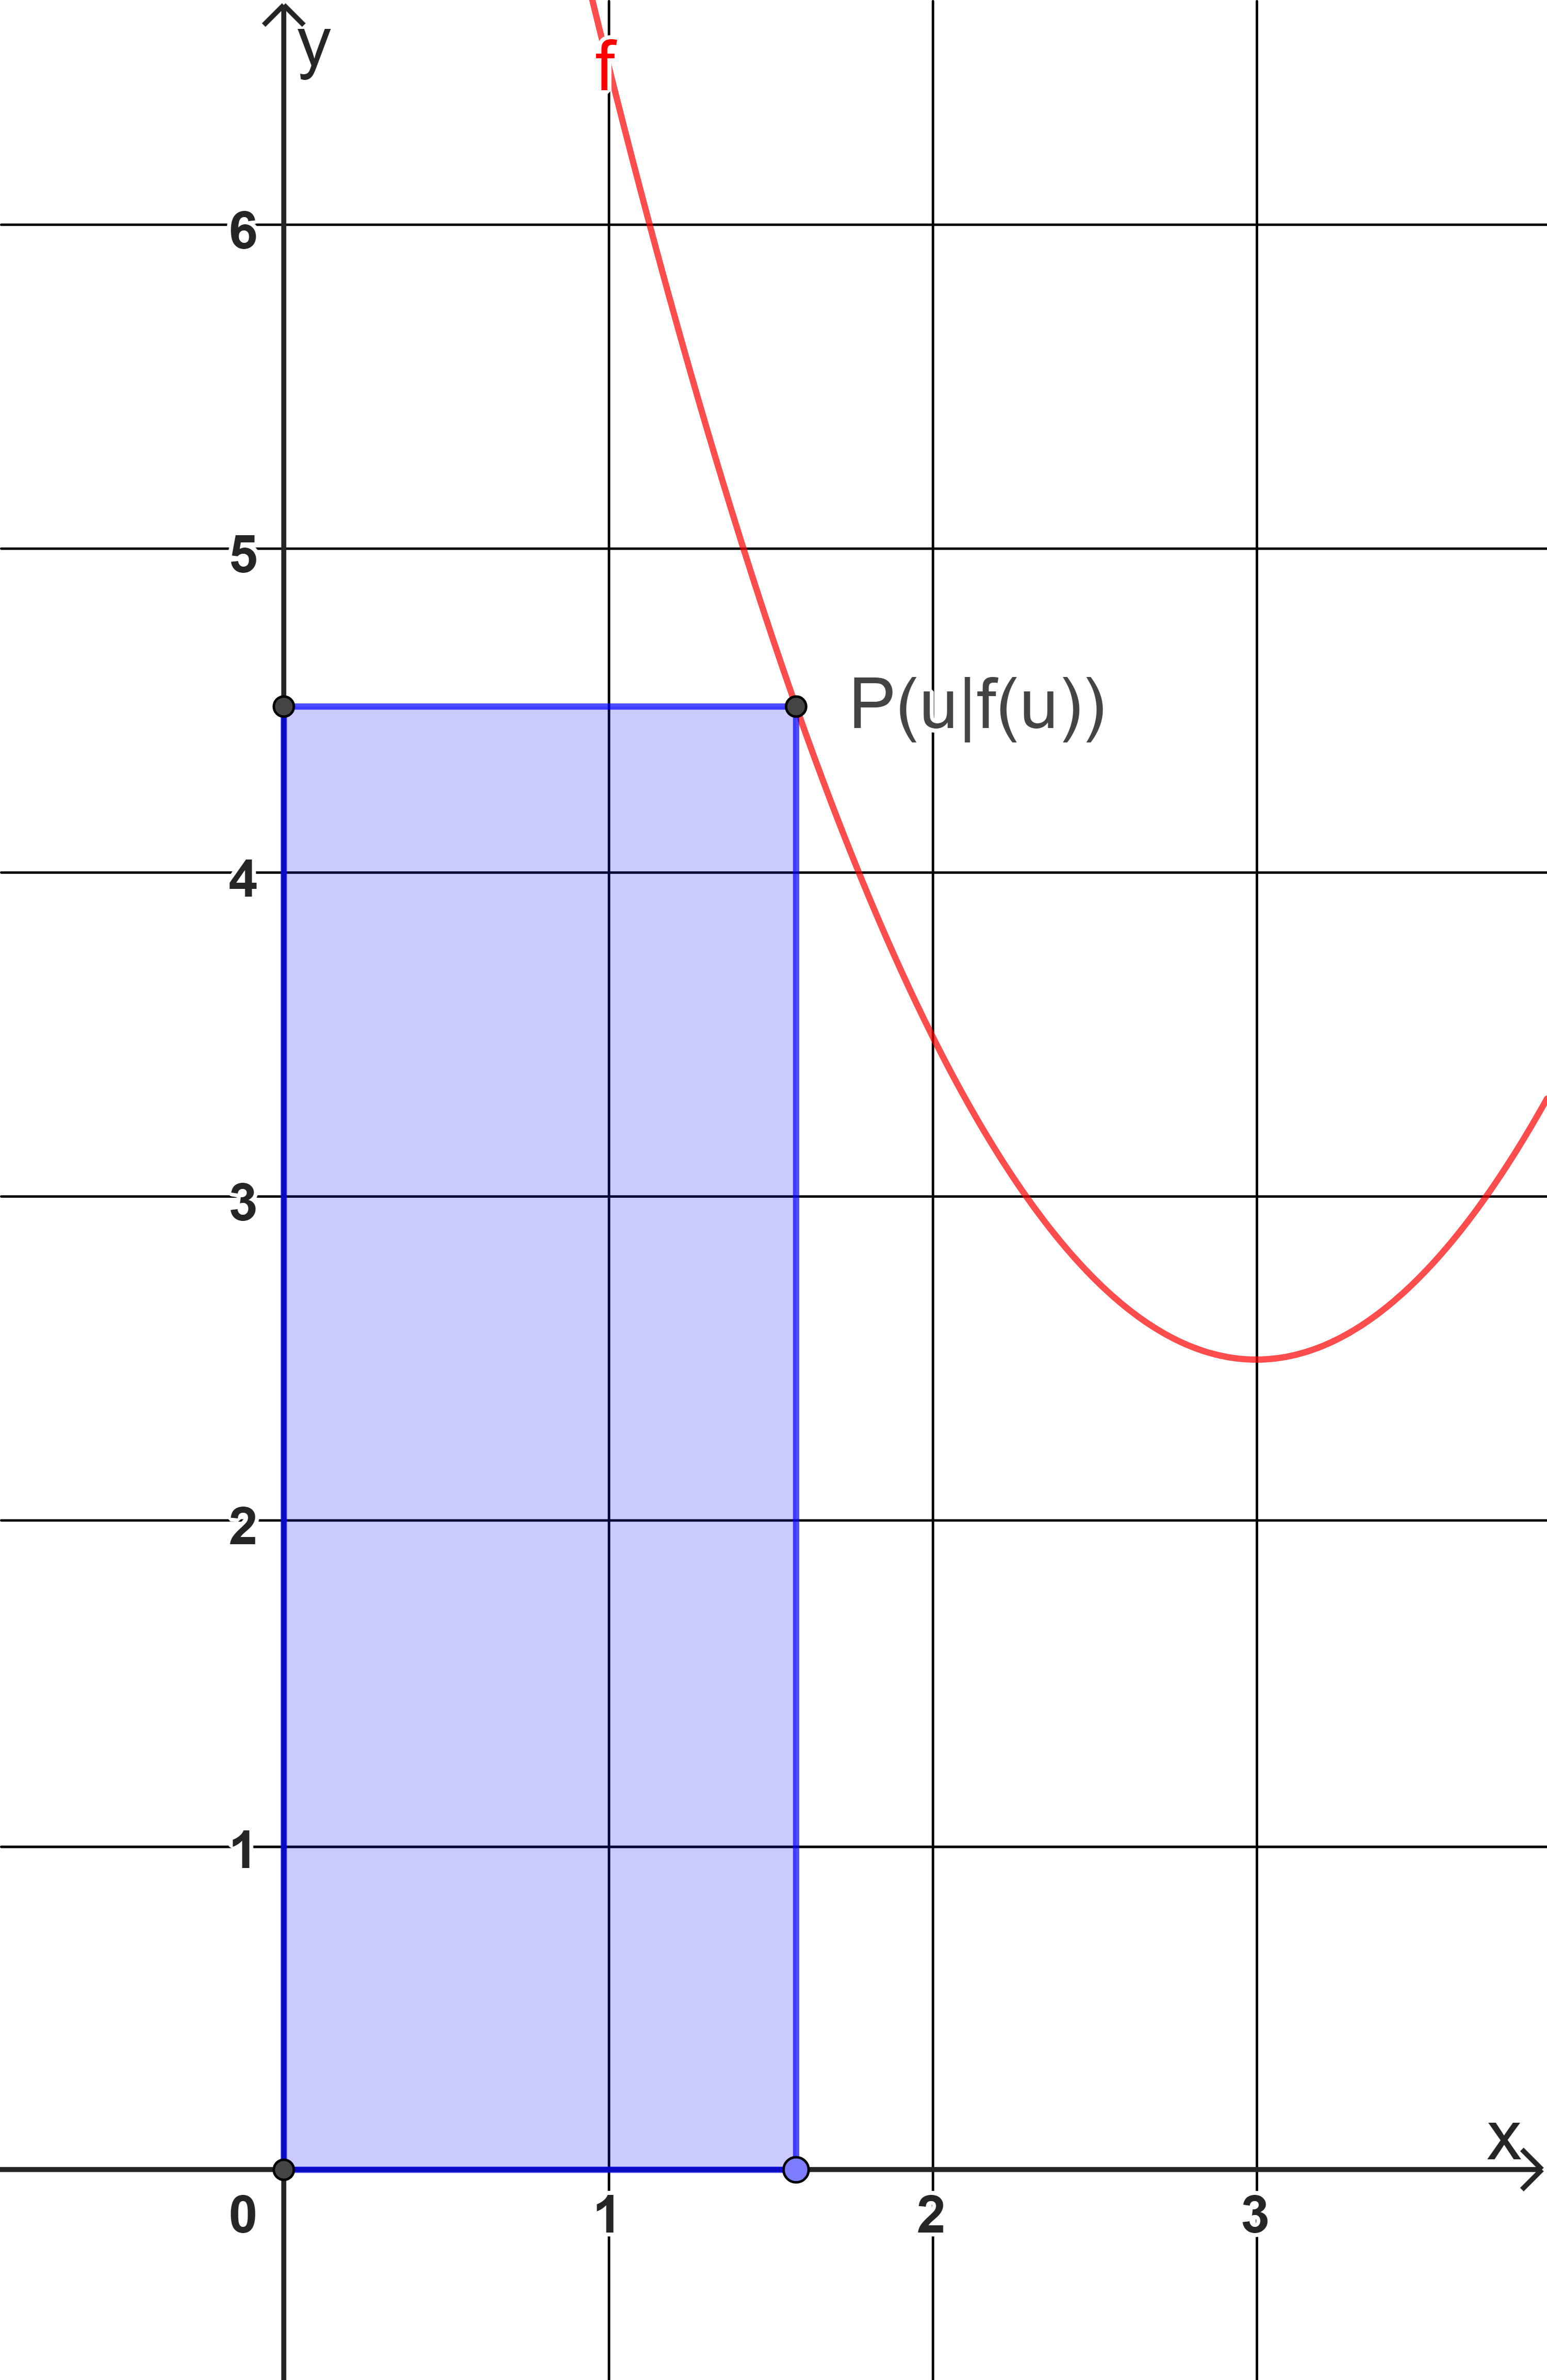
\includegraphics[width=\linewidth]{\optimierung/pics/Aufgabe_4.png}}%
            \setlength{\qrheight}{2.5cm}%
            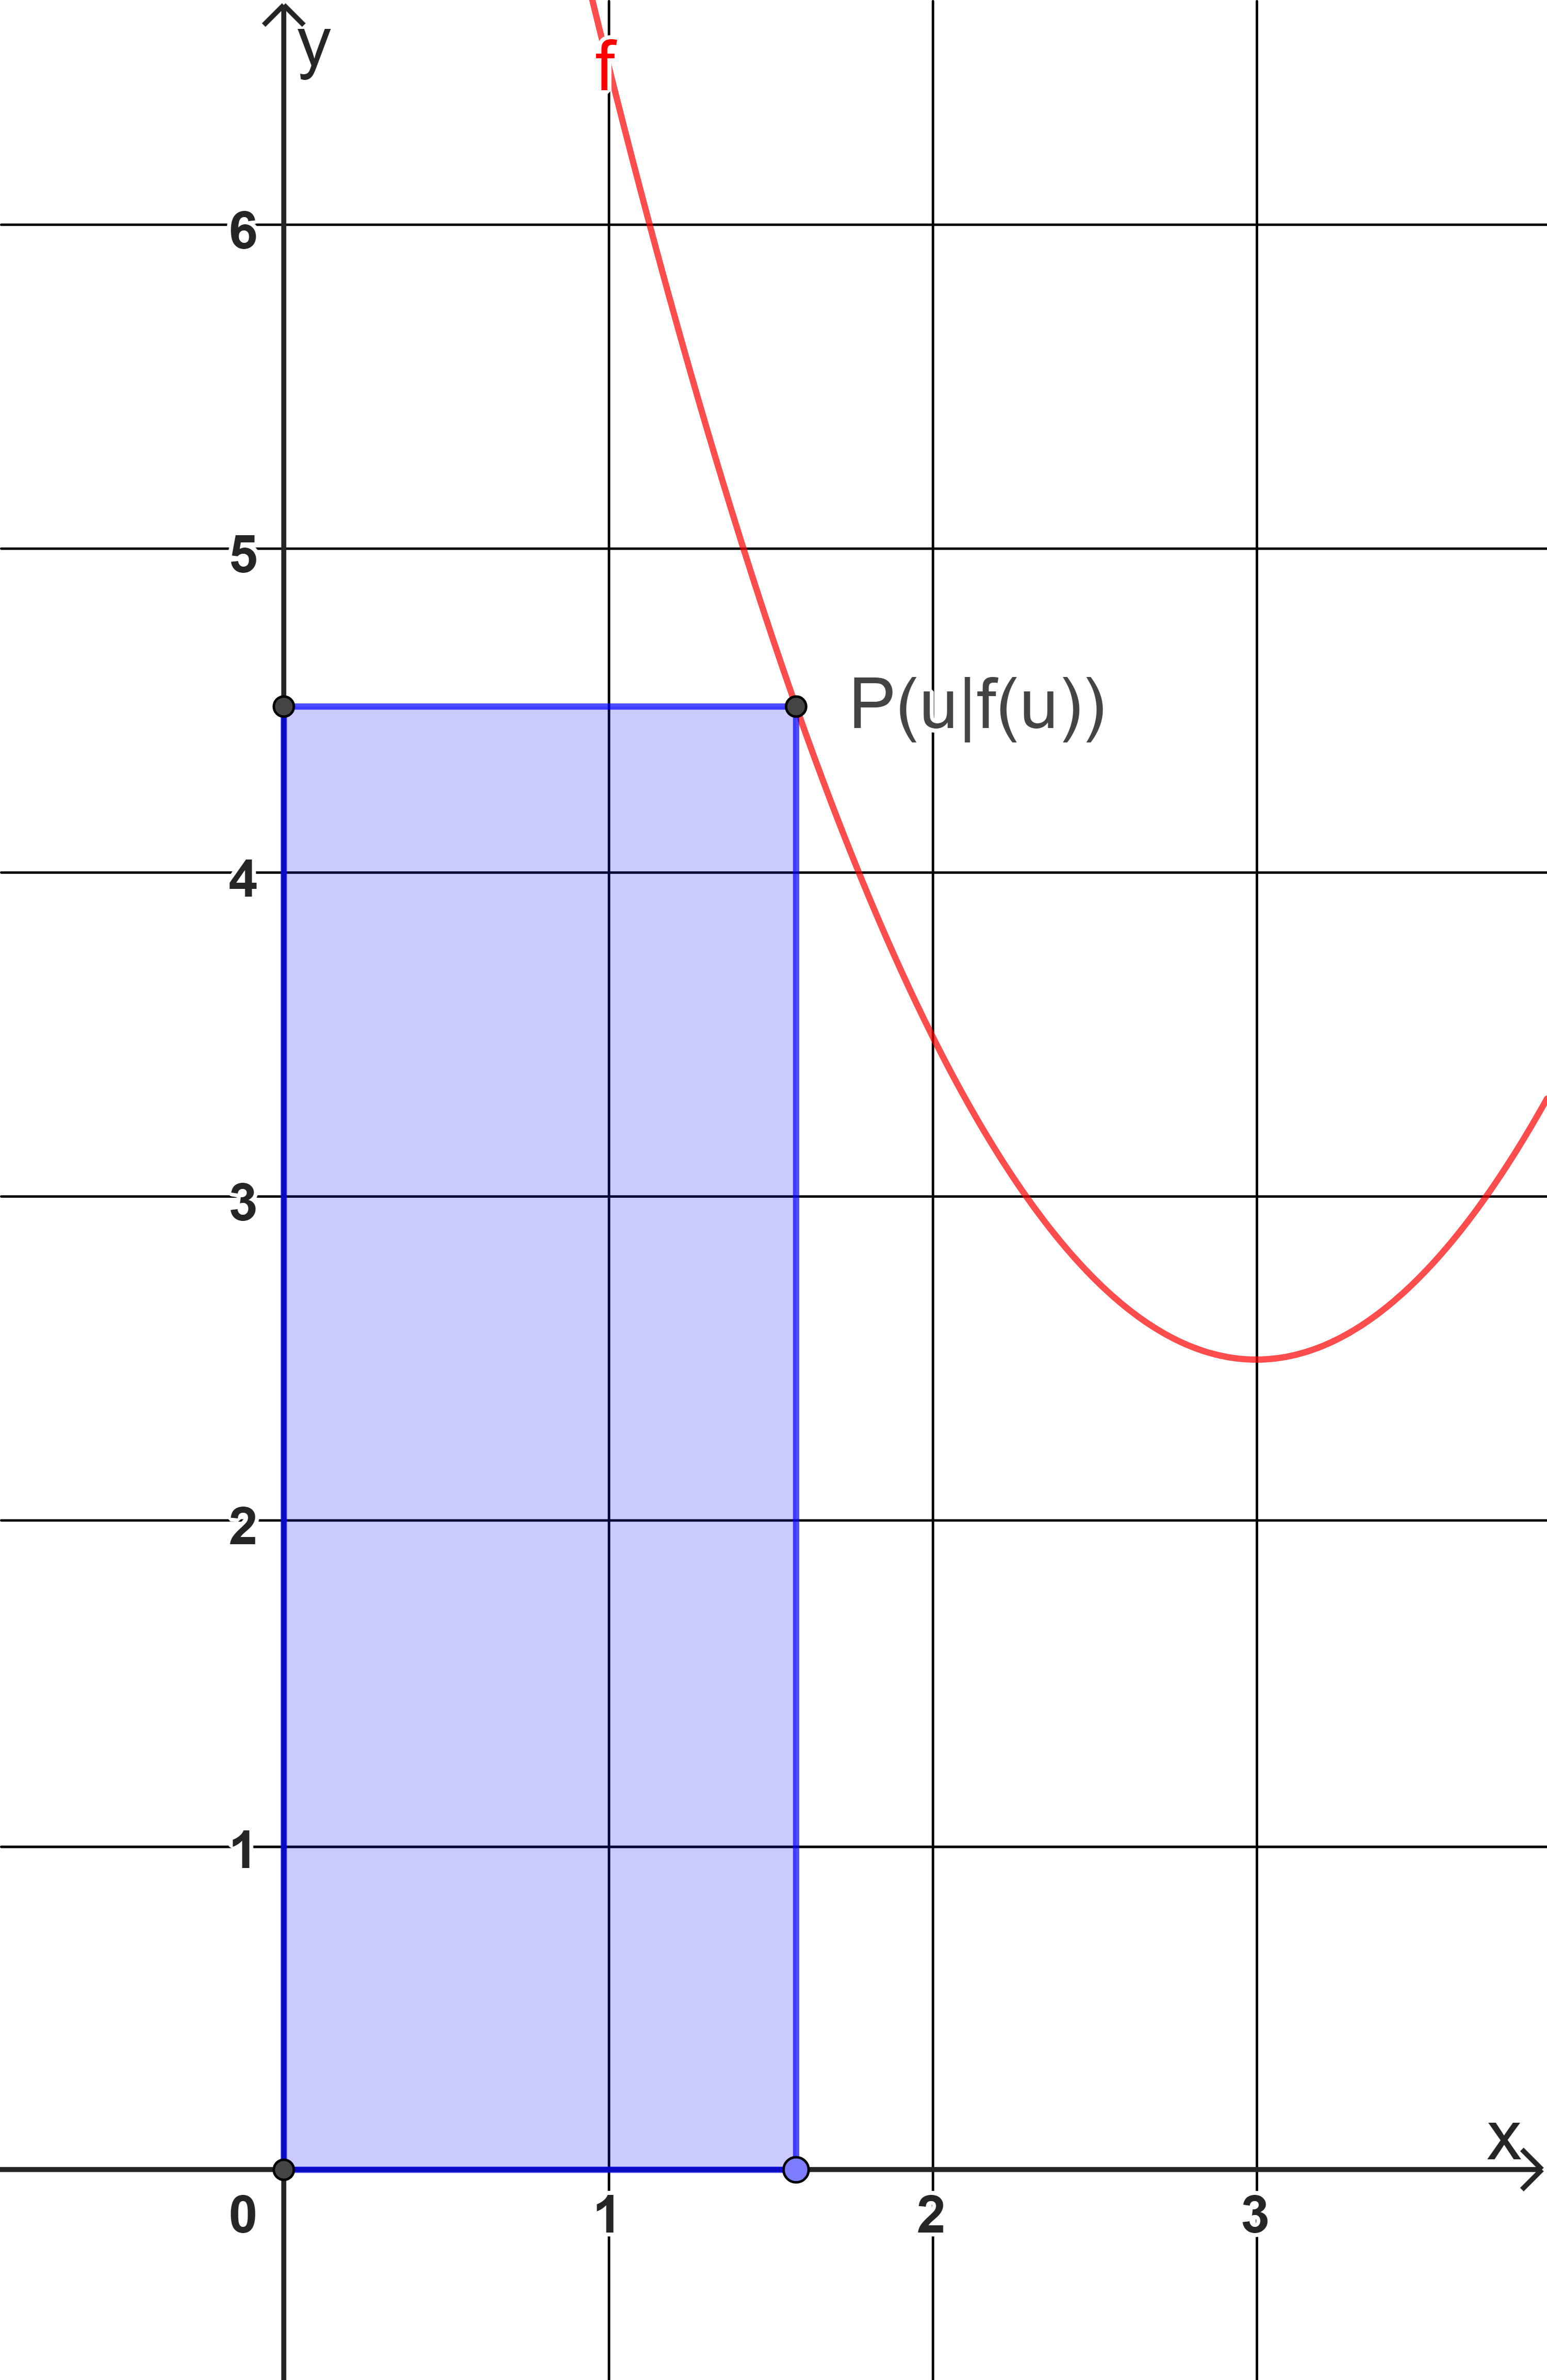
\includegraphics[width=\linewidth]{\optimierung/pics/Aufgabe_4.png}%
            \raisebox{\imgheight-\qrheight}{\makebox[0pt][r]{\href{https://www.geogebra.org/m/ptbksvzz}{
\includegraphics[height=\qrheight]{\optimierung/pics/Aufgabe_4QR.png}}}}%
        }{
            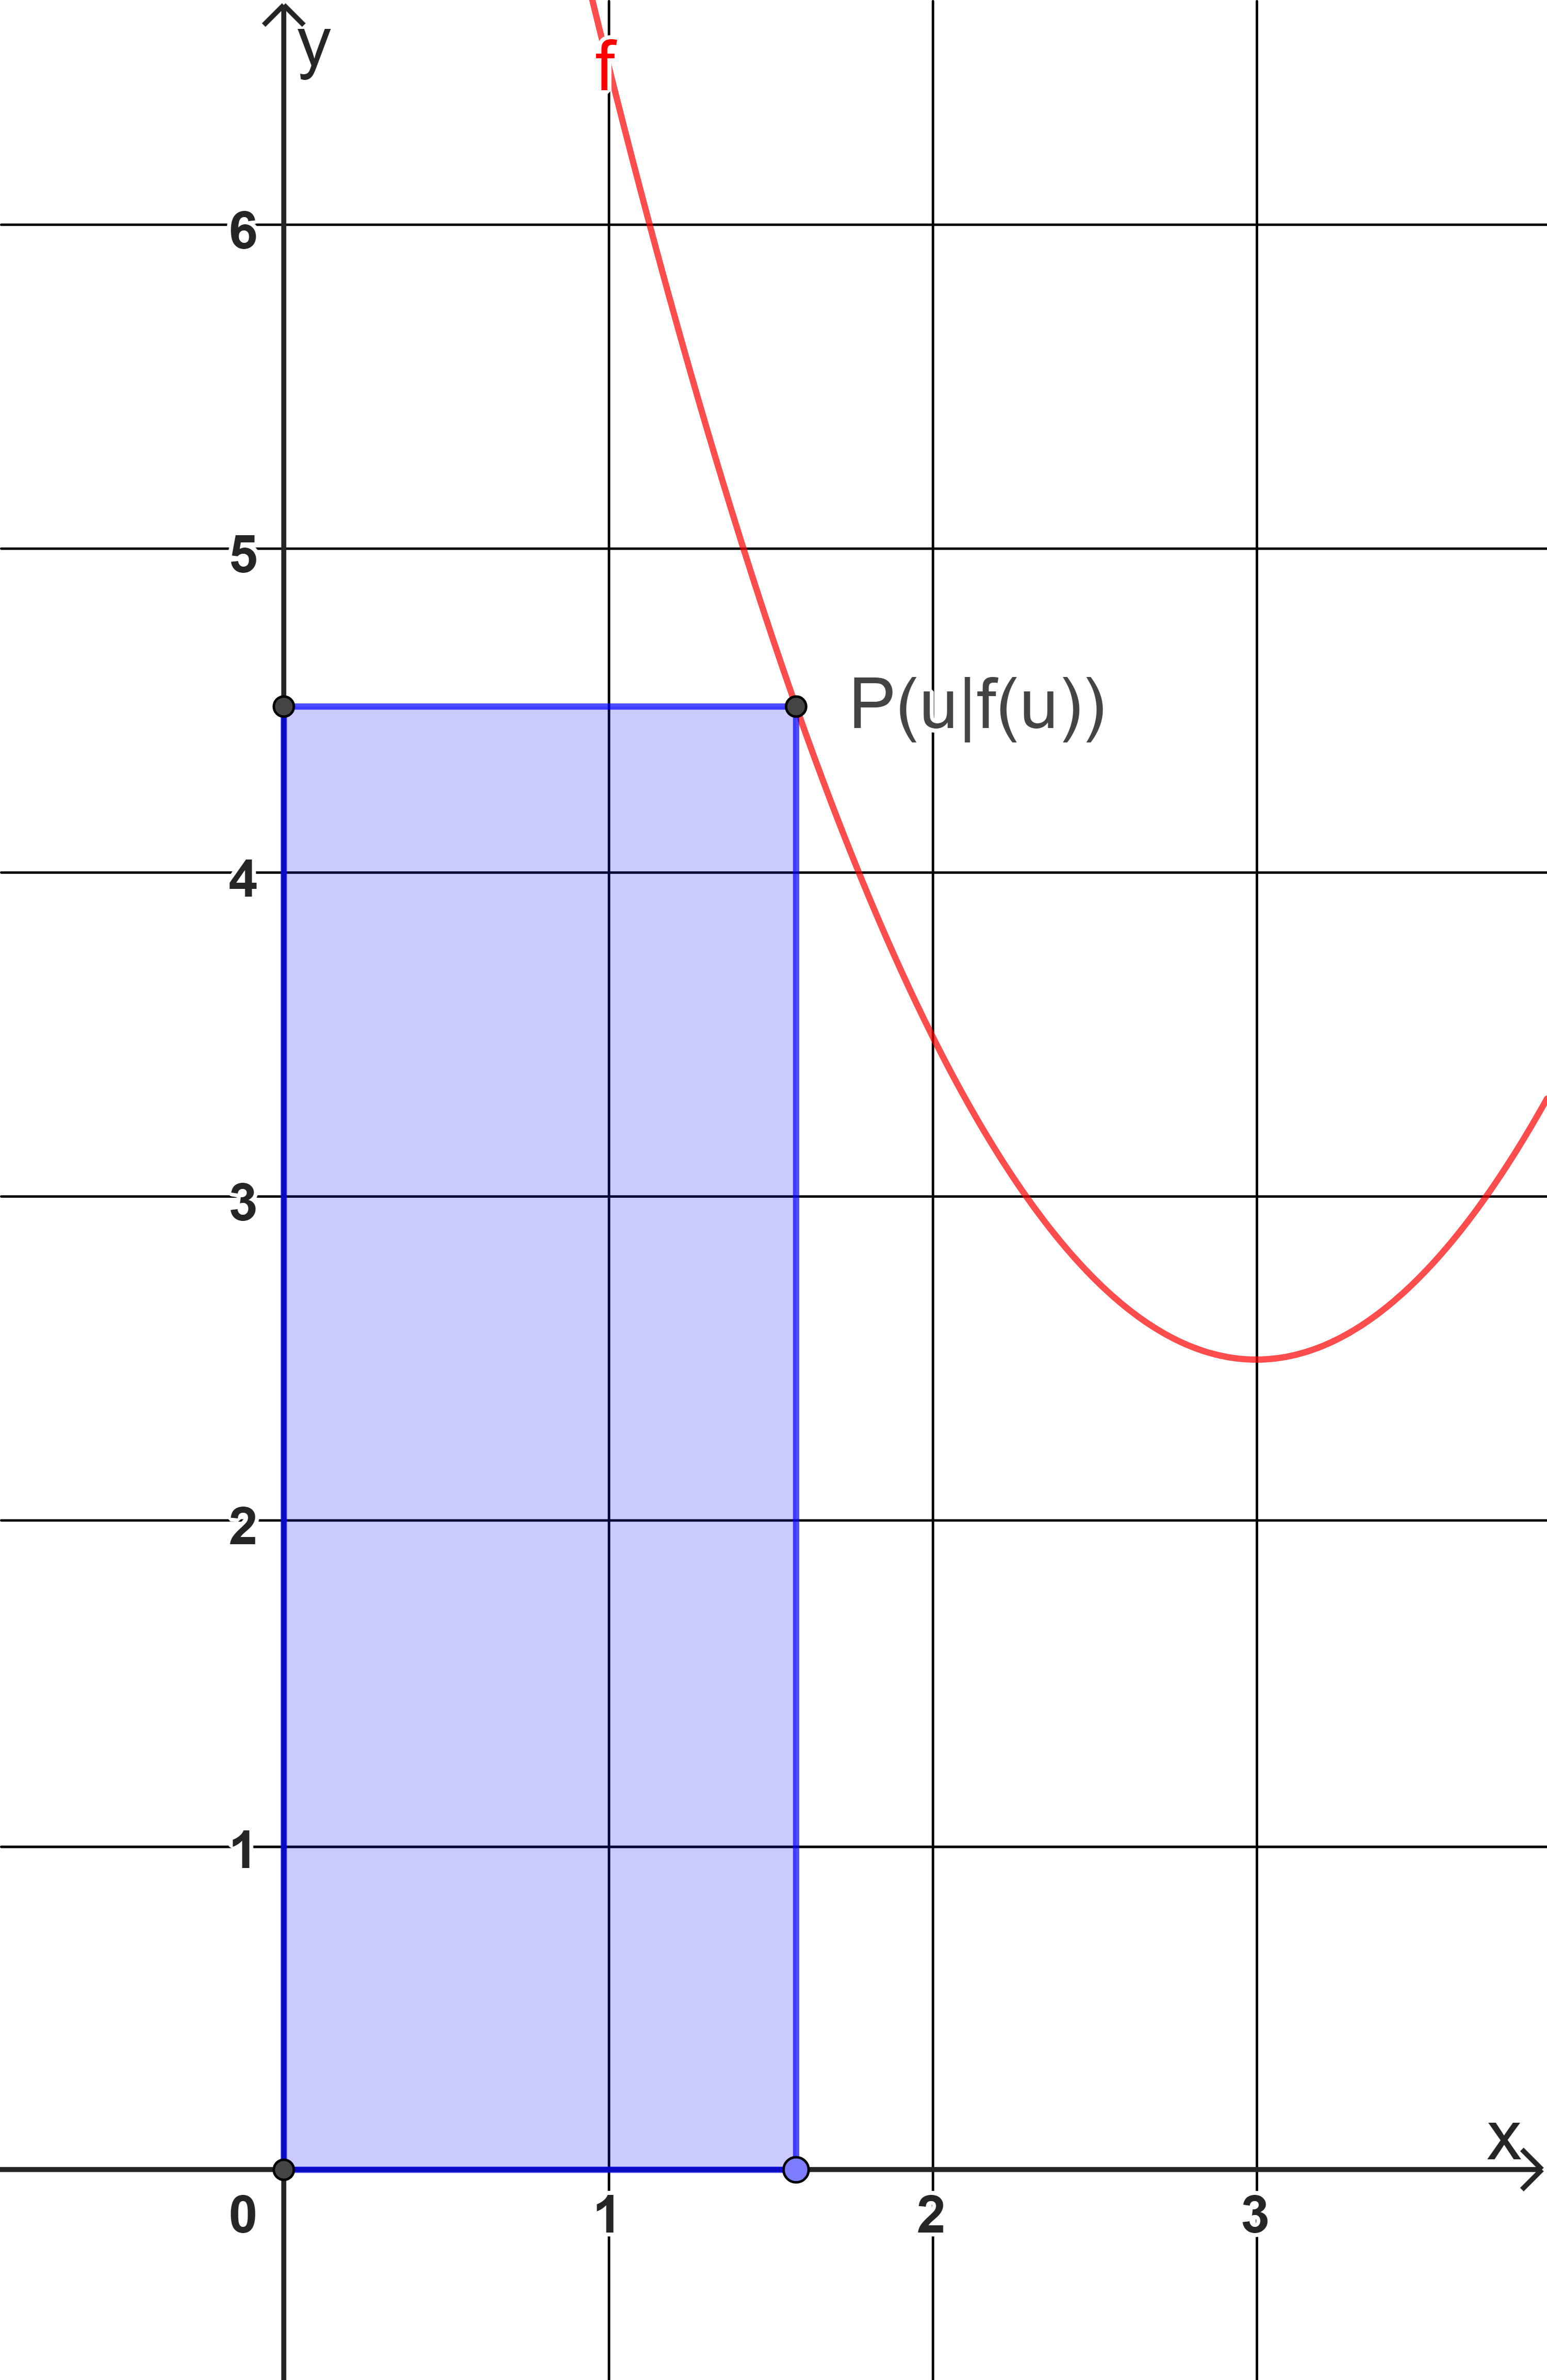
\includegraphics[width=\linewidth]{\optimierung/pics/Aufgabe_4.png}}%
    \end{minipage}}%
	\end{minipage}
\end{Answer}
%%%%%%%%%%%%%%%%%%%%%%%%%%%%%%%%%%%%%%%%%
\begin{Answer}[ref=optimierungA5]

    \bigskip

	\begin{minipage}{\textwidth}
		\adjustbox{valign=t}{\begin{minipage}{.5\textwidth}\raggedright
			\textbf{Zielfunktion}

			\(A(u)=2u\cdot f(u)=-2ku^3+24u\) für \(0\leq u\leq \frac{\sqrt{12}}{k}\)

			Die Einschränkung für \(u\) ergibt sich aus der Tatsache, dass für negative \(u\) die Werte der Zielfunktion negativ werden und für \(u>\frac{\sqrt{12}}{k}\) liegt das Rechteck nicht mehr innerhalb der angegebenen Fläche.

			\textbf{Extremstellen der Zielfunktion}

			\(A'(u)=-6ku^2+24\)

			\(A''(u)=-12ku\)

			\(A'(u)=0\) liefert \(u_{1/2}=\pm\frac{2}{\sqrt{k}}\).

			Die negative Lösung liegt nicht im erlaubten Bereich und kann ignoriert werden.

			Mit \(A''\left(\frac{2}{\sqrt{k}}\right)=-24\sqrt{5}<0\) liegt bei der positiven Lösung ein Hochpunkt.

			\textbf{Antwort erstellen}

			Der maximale Flächeninhalt beträgt \(A\left(\frac{2}{\sqrt{k}}\right)=\frac{32}{\sqrt{k}}\).

			Die Eckpunkte sind dann
			\(A\left( \frac{2}{\sqrt{k}}\middle\vert 0\right),
			\ B\left( \frac{2}{\sqrt{k}}\middle\vert f\left(\frac{2}{\sqrt{k}}\right)=8\right),\newline
			C\left(-\frac{2}{\sqrt{k}}\middle\vert 8\right),
			\ D\left(-\frac{2}{\sqrt{k}}\middle\vert 0\right)\).
		\end{minipage}}%
        \adjustbox{valign=t, padding = 2ex 0ex 0ex 0ex}{\begin{minipage}{.5\textwidth-2ex}                \iftoggle{qrcode}{
            \settototalheight{\imgheight}{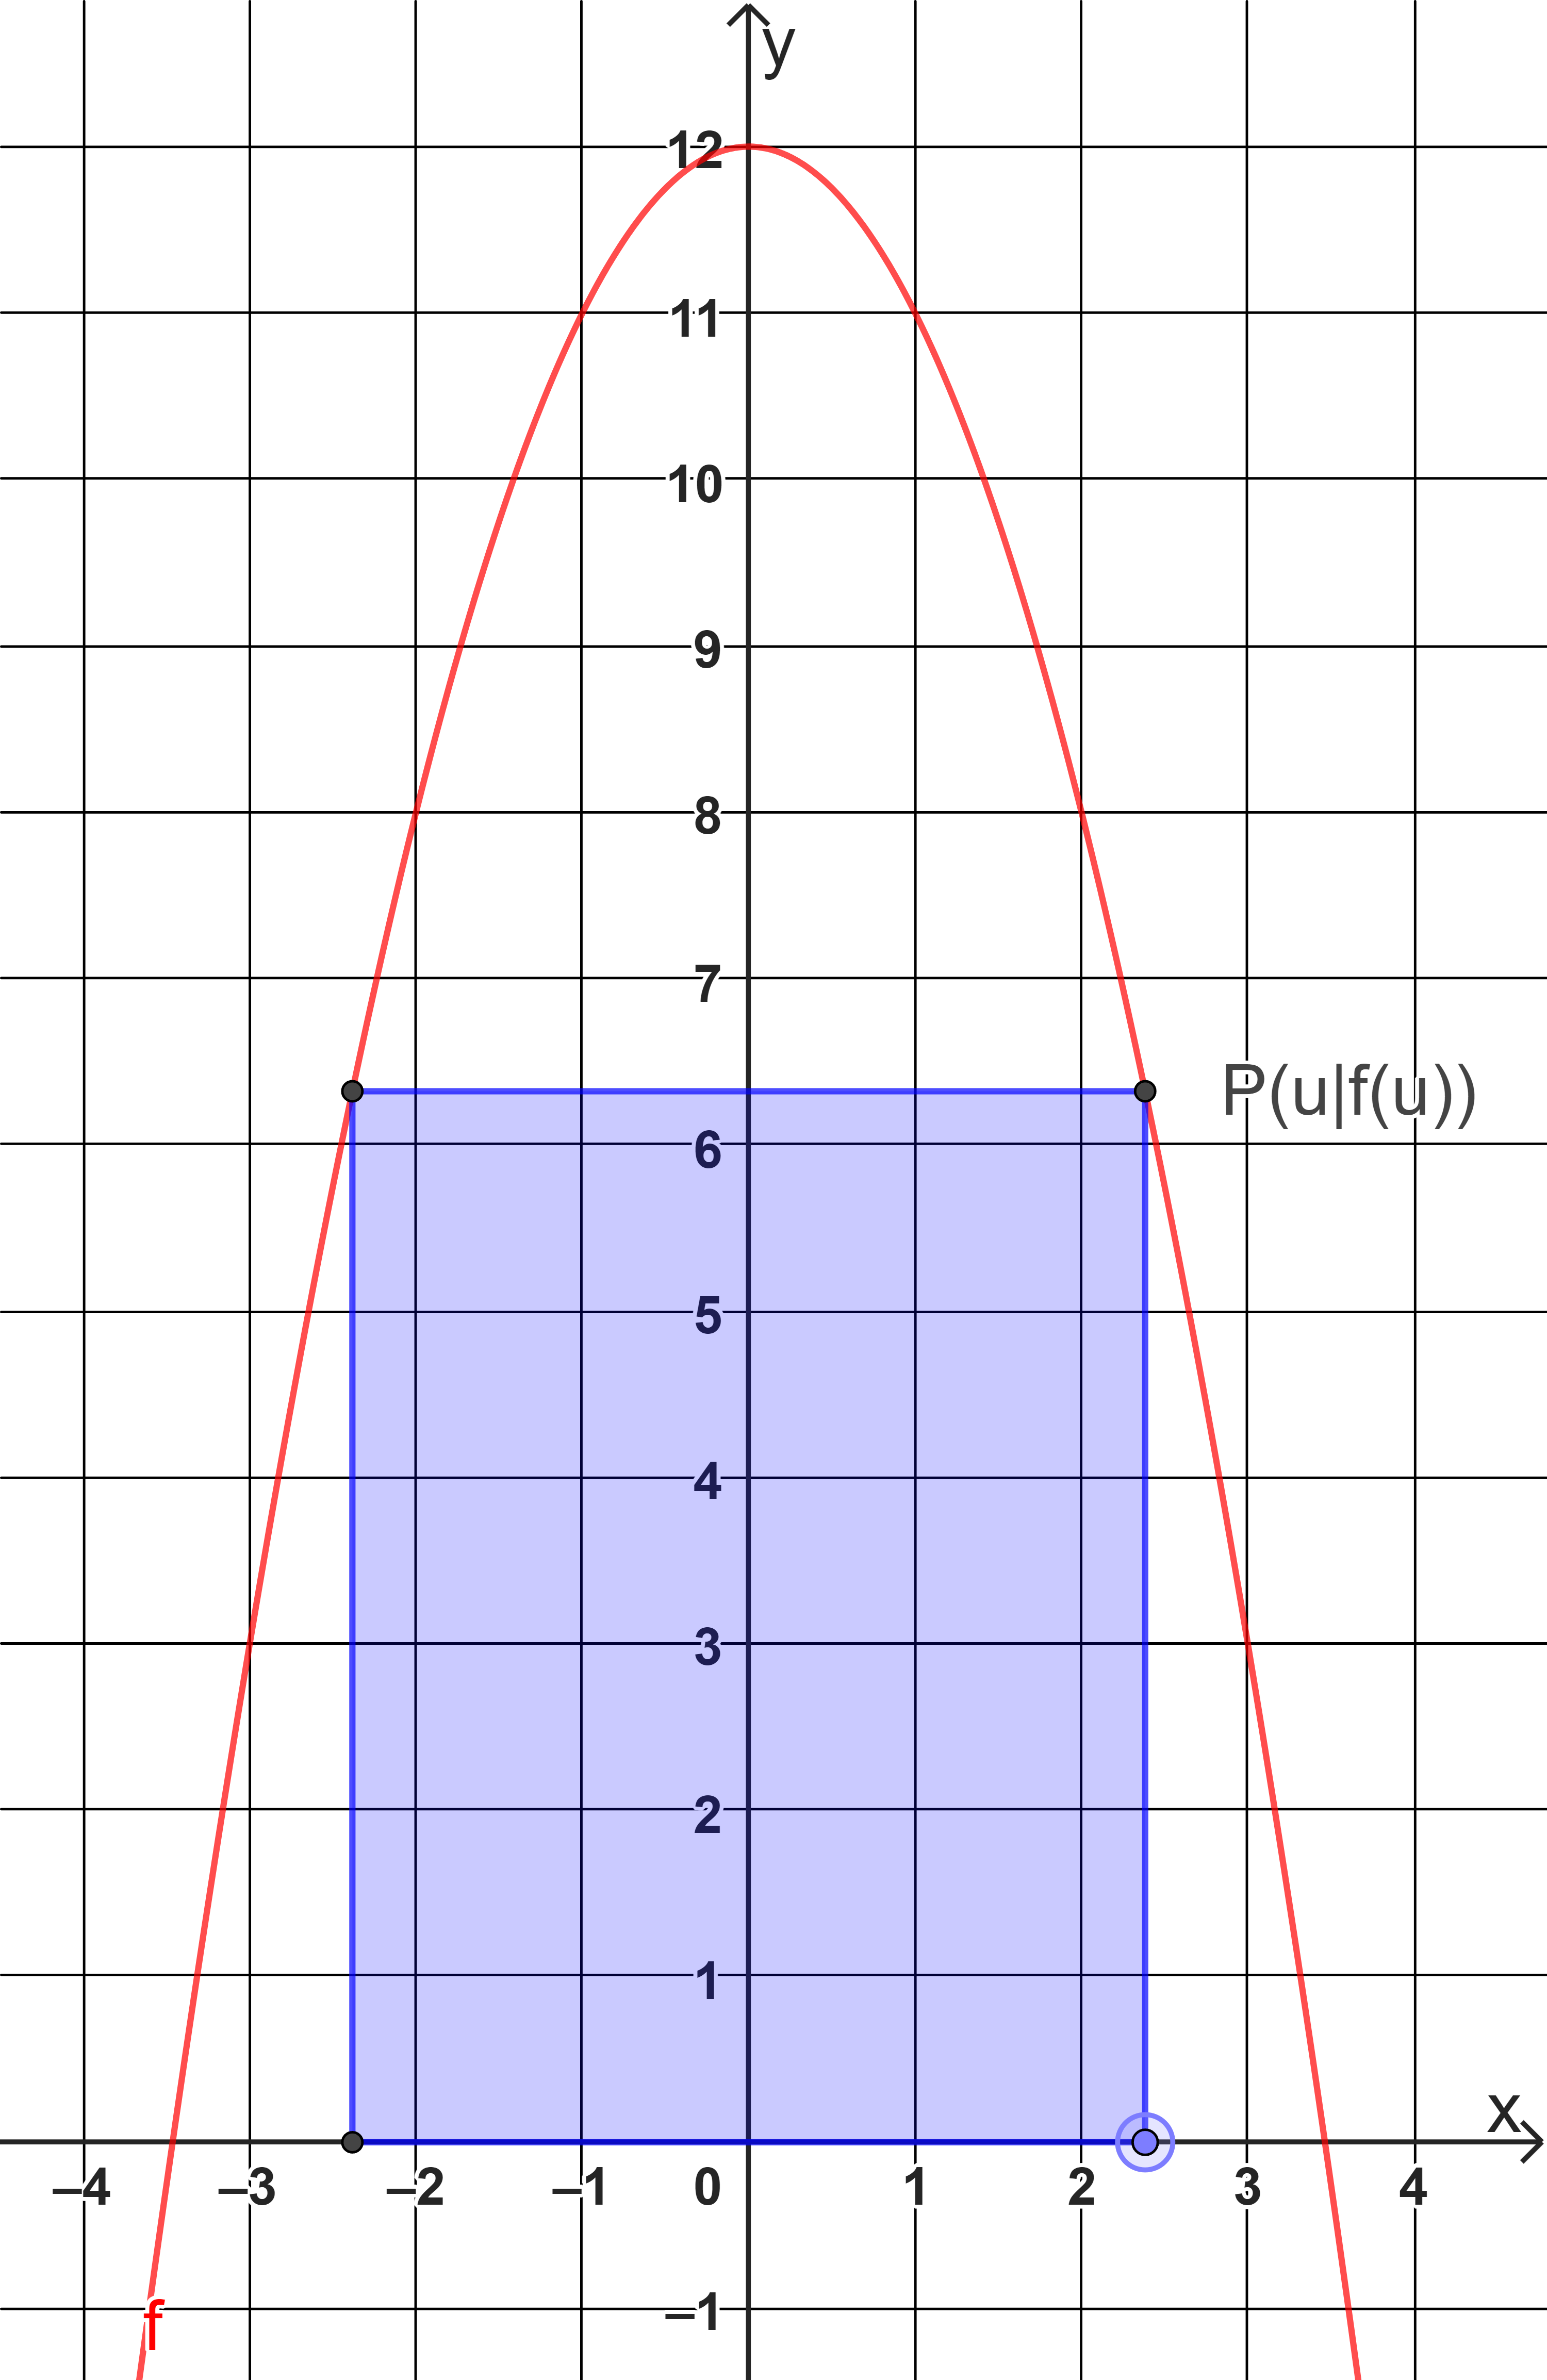
\includegraphics[width=\linewidth]{\optimierung/pics/Aufgabe_5.png}}%
            \setlength{\qrheight}{2.5cm}%
            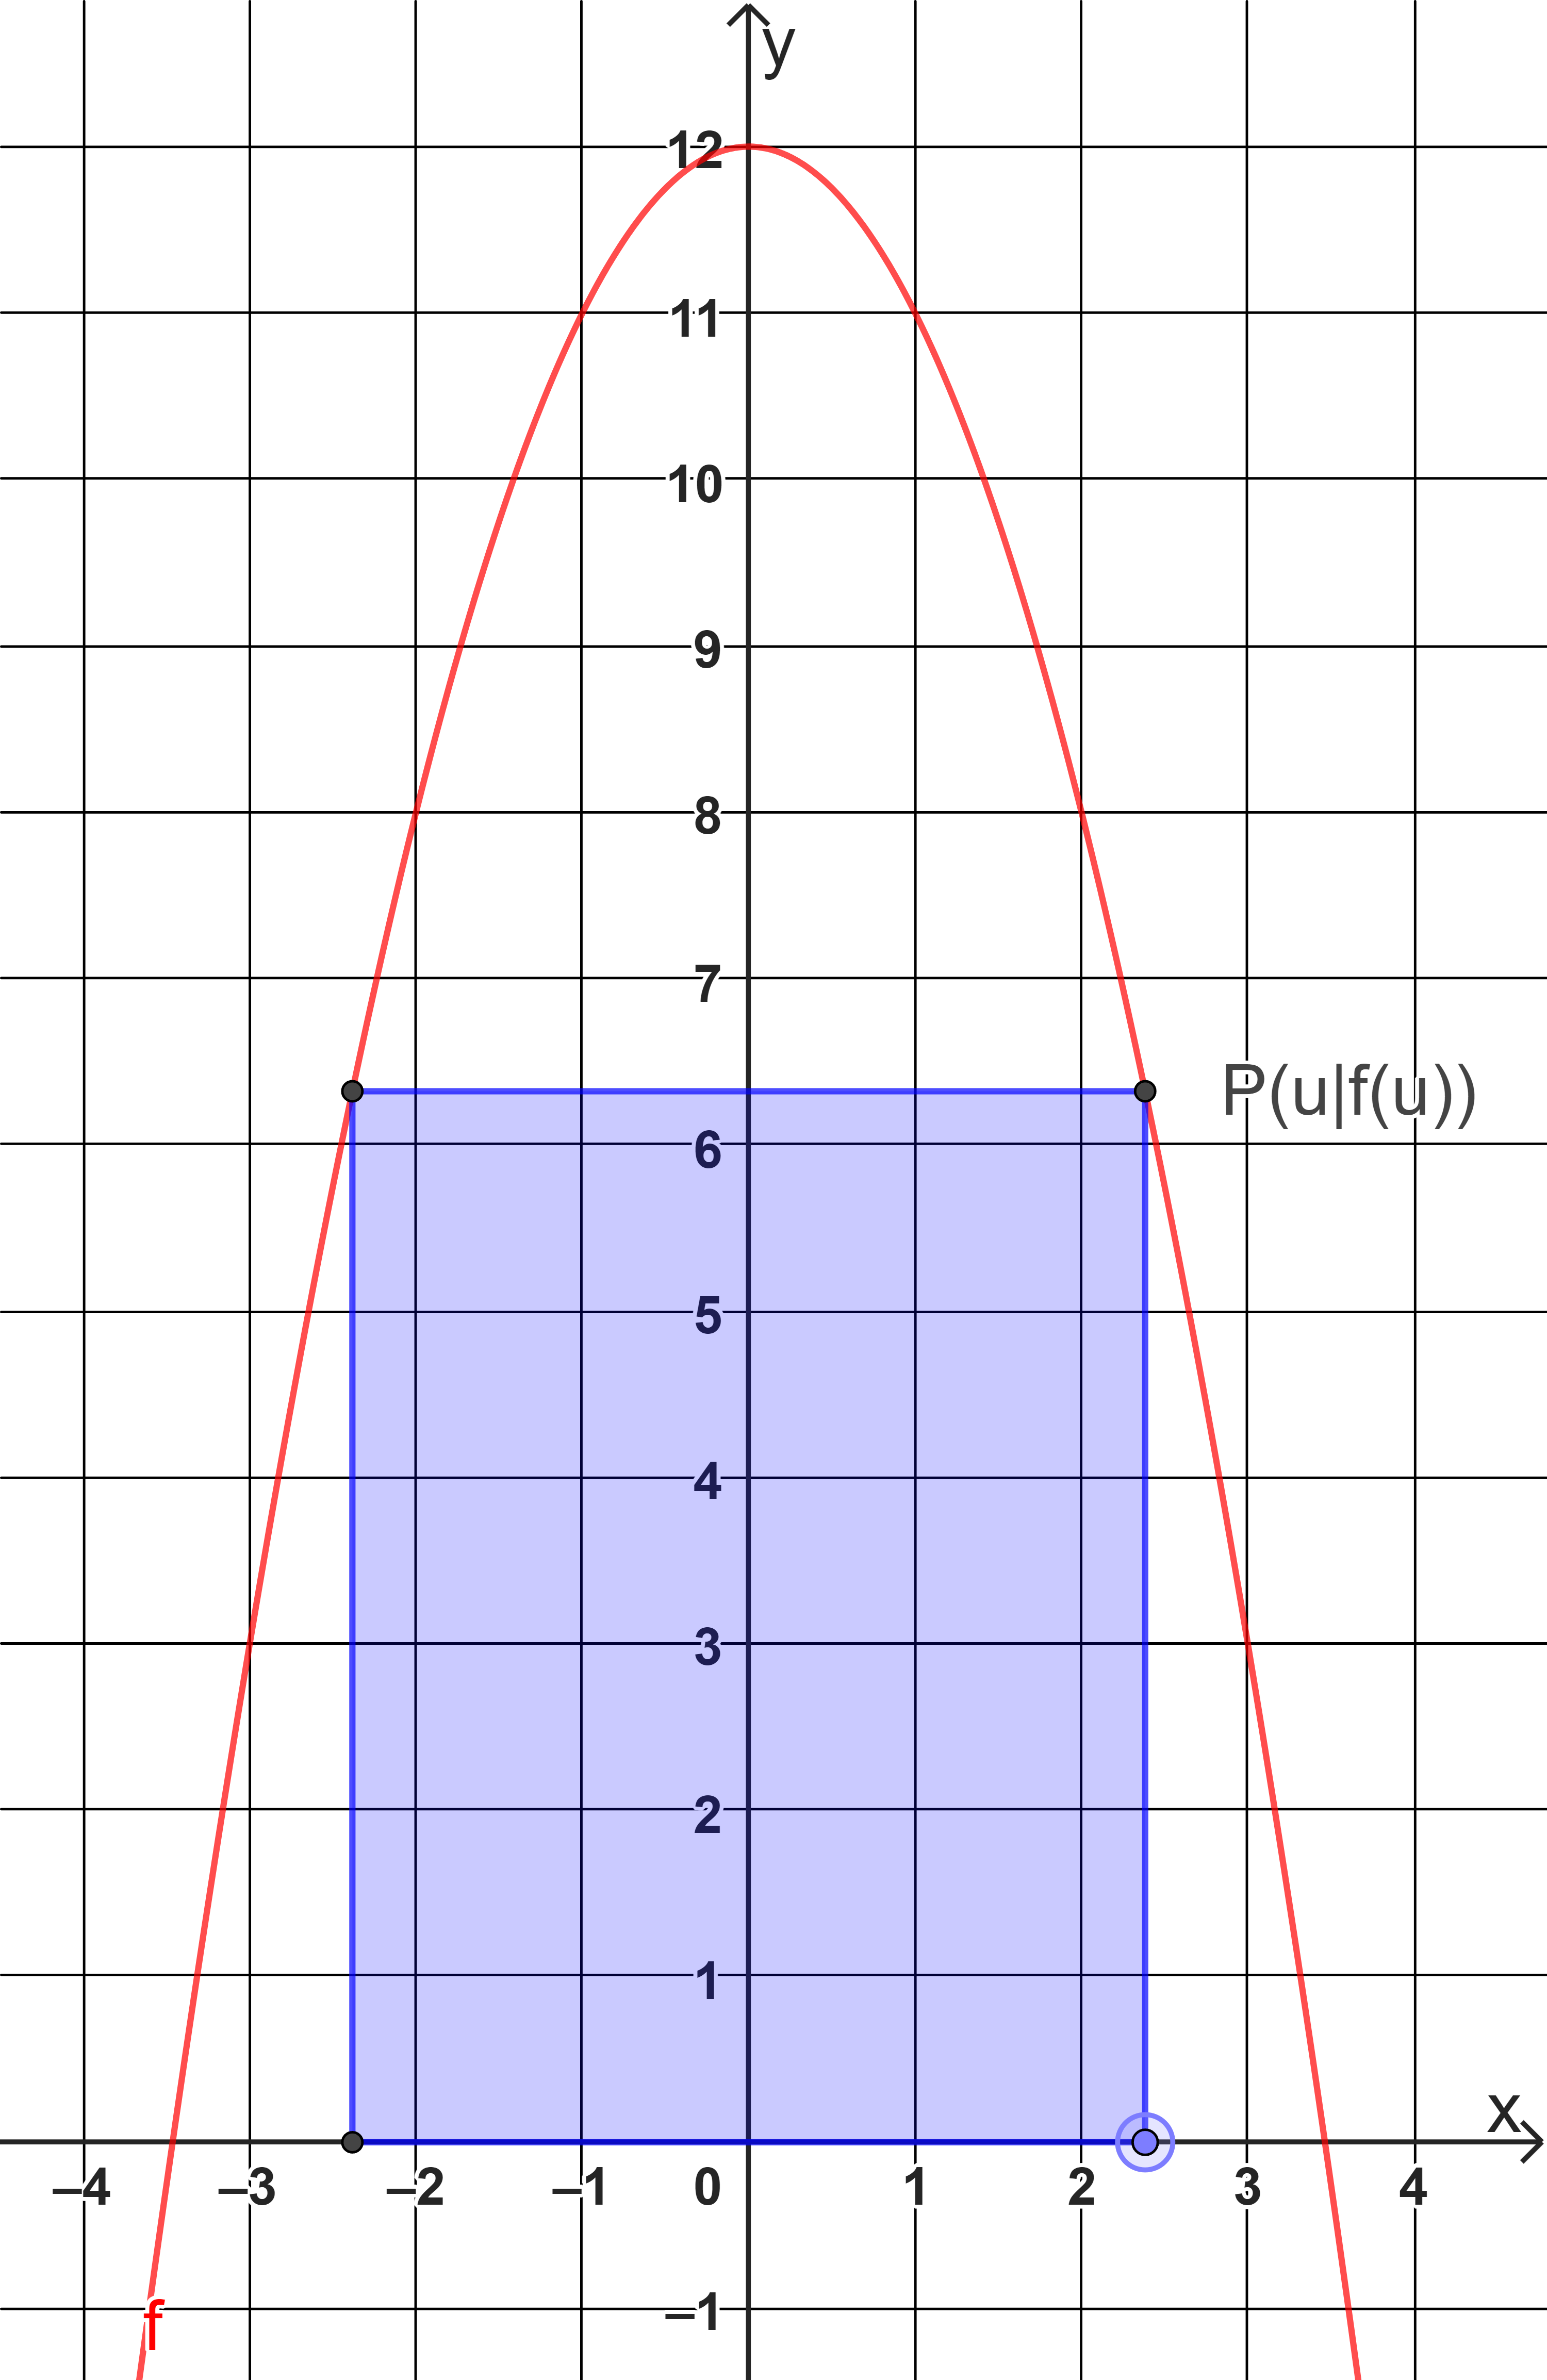
\includegraphics[width=\linewidth]{\optimierung/pics/Aufgabe_5.png}%
            \raisebox{\imgheight-\qrheight}{\makebox[0pt][r]{\href{https://www.geogebra.org/m/wuxpt9u8}{
\includegraphics[height=\qrheight]{\optimierung/pics/Aufgabe_5QR.png}}}}%
        }{
            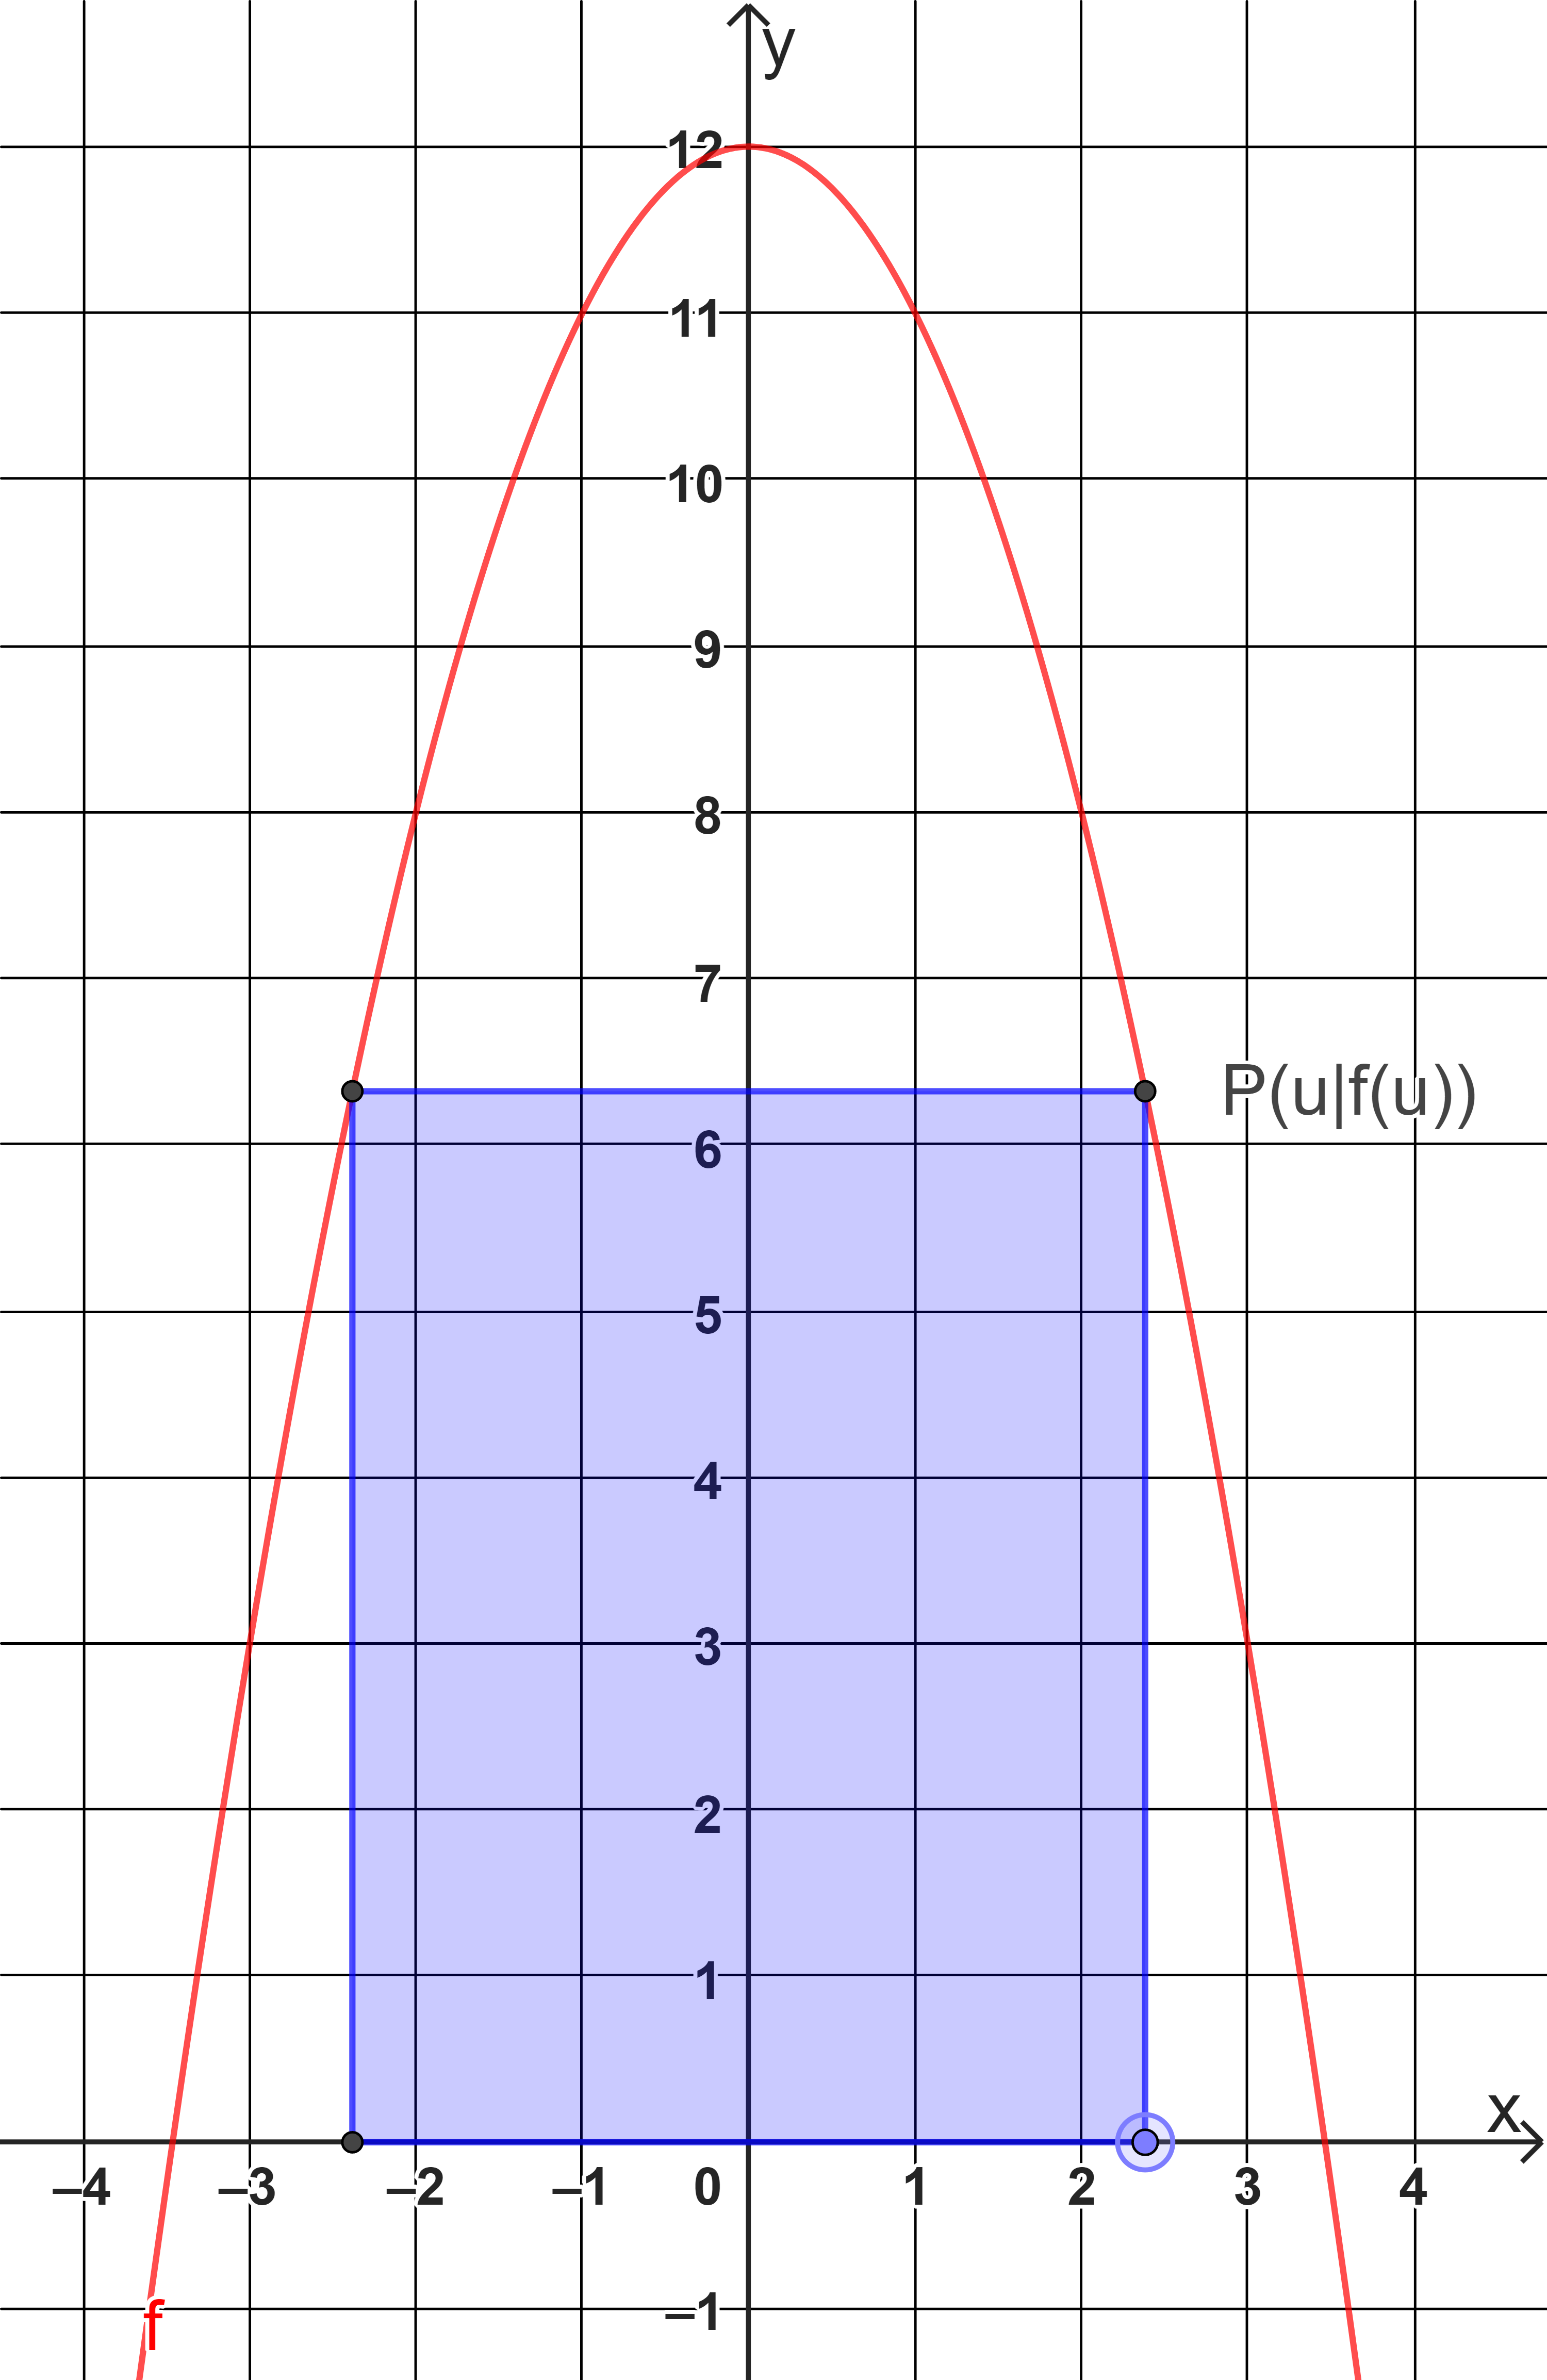
\includegraphics[width=\linewidth]{\optimierung/pics/Aufgabe_5.png}}%
        \end{minipage}}%
	   \end{minipage}
\end{Answer}